\chapter{DESAIN DAN IMPLEMENTASI SISTEM}
\vspace{4ex}

\hspace{\parindent} Penelitian ini dilaksanakan sesuai dengan desain sistem serta implementasinya. Desain sistem merupakan konsep dari pembuatan dan perancangan infrastruktur kemudian diwujudkan dalam bentuk blok-blok alur yang harus dikerjakan. Implementasi merupakan pelaksanaan teknis untuk setiap blok pada desain sistem.
\vspace{2ex}

\section{Gambaran Umum}
\vspace{1ex}
	Penelitian ini bertujuan untuk merancang dan menerapkan interaksi berdasarkan \textit{hand gesture} pada hologram 3D. Sistem ini dikemas dalam satu set yang terdiri dari \textit{pyramid hologram}, Leap Motion, \textit{display monitor}, \textit{information monitor} beserta \textit{server computer} seperti pada gambar \ref{fig:cara_kerja}.
	\begin{figure} [H]
		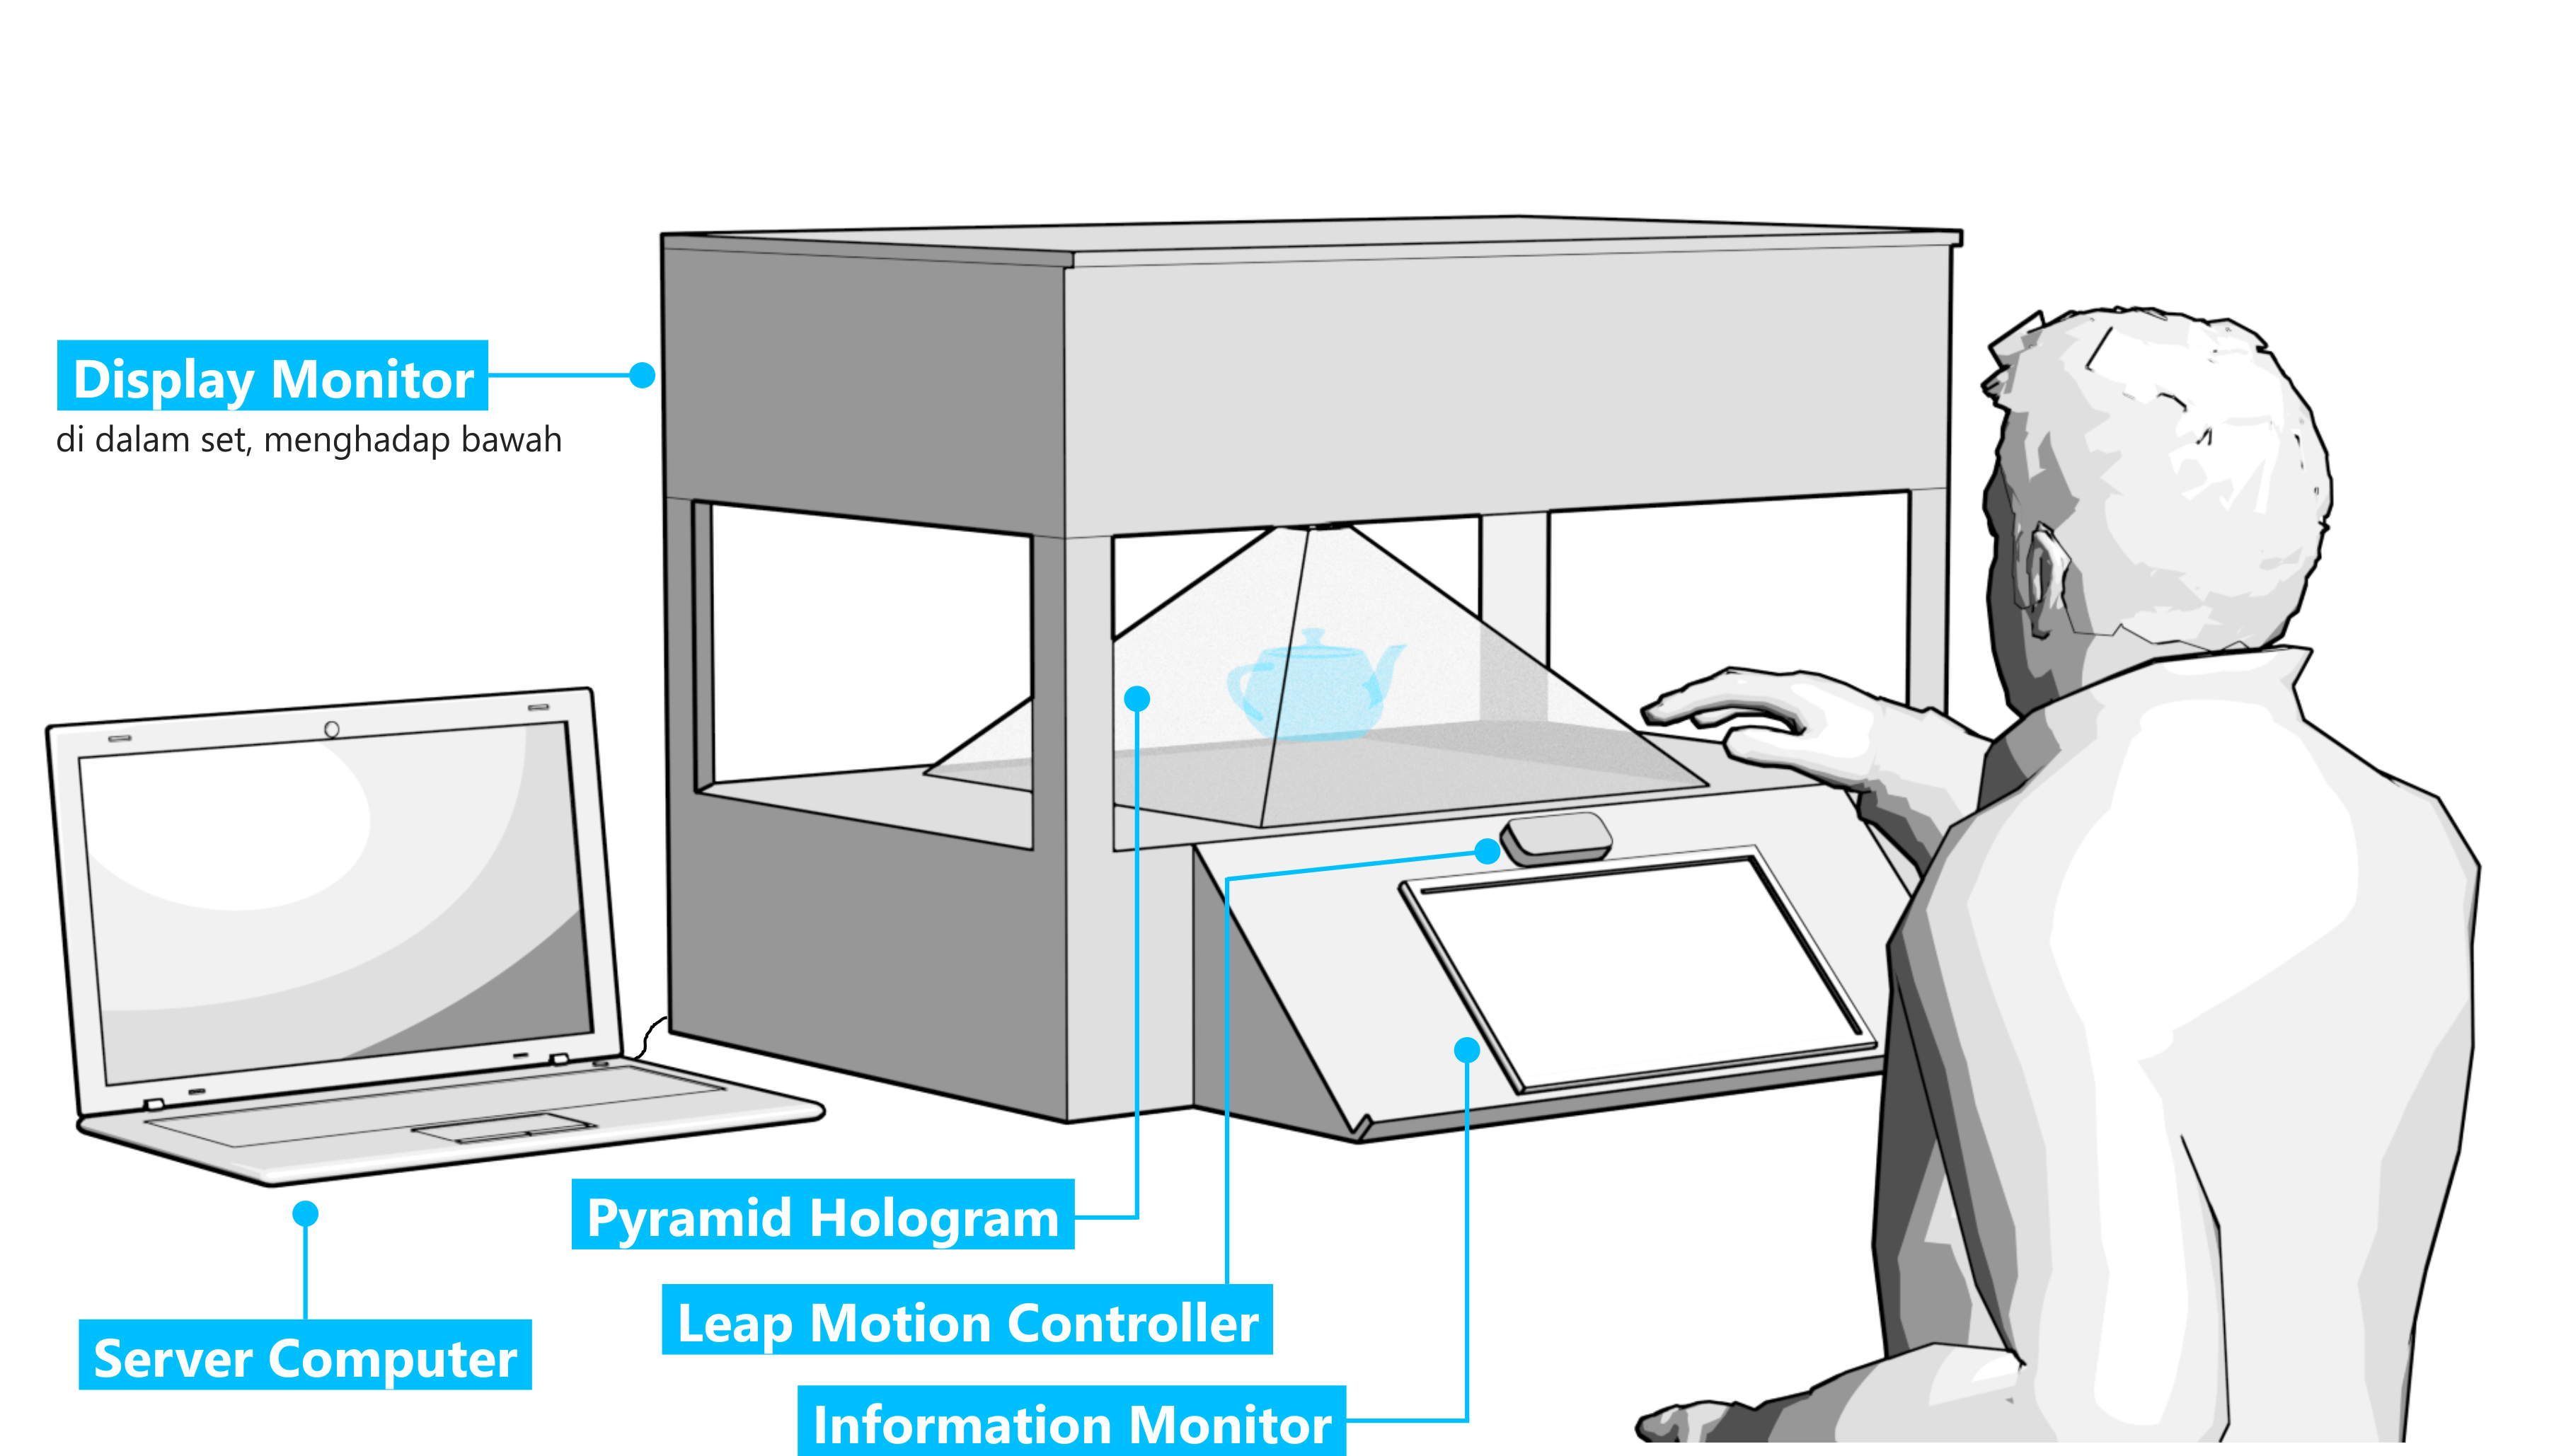
\includegraphics[width=\textwidth]{img/bab3/cara_kerja.png}
		\caption{Gambaran umum penggunaan sistem.}
		\label{fig:cara_kerja}
	\end{figure}
	\textit{Display monitor} dan \textit{pyramid hologram} di bawahnya menampilkan objek hologram 3D sedangkan \textit{information monitor} menampilkan informasi mengenai program yang dijalankan. Leap Motion yang terletak di atas \textit{information monitor} menangkap pergerakan tangan pengguna. \textit{Server computer}  mengolah data dan menentukan fitur yang diaktifkan. Berdasarkan data yang diperoleh maka objek hologram dapat menampilkan respons dan memungkinkan pengguna melakukan interaksi.
\vspace{2ex}

\section{Desain Sistem}
\vspace{1ex}
	Pada sistem ini pengguna dapat melakukan interaksi dengan hologram menggunakan Leap Motion. Objek hologram yang diperlihatkan melalui pantulan dari monitor terhadap \textit{pyramid hologram} dapat merespons sesuai \textit{hand gesture} dari pengguna. Kemudian informasi mengenai objek hologram tersebut juga ditampilkan. Alur kerja dari sistem ini dijelaskan melalui gambar \ref{fig:alur_kerja}.
	\vspace{-2ex}
	\begin{figure} [H]
		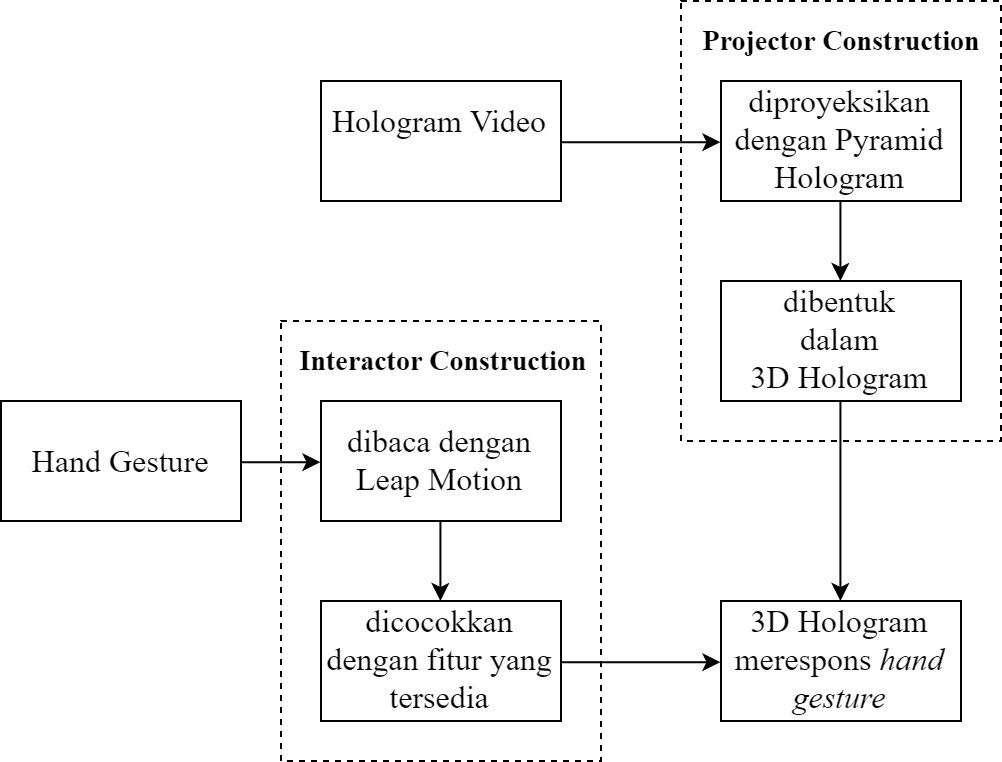
\includegraphics[scale=0.25]{img/bab3/alur_kerja.png}
		\caption{Alur kerja penggunaan sistem.}
		\label{fig:alur_kerja}
	\end{figure}
	\vspace{-2ex}
	Terdapat dua sub-sistem yang membangun tujuan dari penelitian ini, yaitu sistem virtualisasi mengenai pembangunan aplikasi termasuk rekonstruksi objek 3D menjadi bentuk hologram maupun \textit{user interface} untuk informasinya dan sistem interaksi tentang bagaimana pengguna dapat memberikan input terhadap objek hologram. Agar kedua sub-sistem ini dapat berfungsi bersamaan, maka dibutuhkan perancangan desain \textit{storyboard} penggunaan serta setting perangkat.
\vspace{1.5ex}

	\subsection{Desain \textit{Storyboard}}
	\vspace{1ex}
		\textit{Storyboard} yang diterapkan pada penelitian ini dirancang berdasarkan alur yang akan dilakukan oleh pengguna saat menggunakan perangkat. Alur penggunaan perangkat ini dijelaskan melalui tahapan sebagai berikut :
		\begin{enumerate}[nolistsep]
			\item Ketika pengguna menggunakan perangkat, kedua monitor menampilkan bagian awal aplikasi. \textit{Display monitor} menampilkan sebuah objek hologram yang berputar. Sedangkan \textit{information monitor} menampilkan \textit{Main Menu} aplikasi.
			\item Ketika memilih tombol "Start", kedua monitor memberikan panduan mengenai cara penggunaan dan gestur dasar yang dibangun pada sistem ini.
			\item Setelah menyelesaikan tutorial panduan, kedua monitor menampilkan koleksi objeknya satu persatu.  Objek-objek yang ditampilkan secara berurutan adalah \textit{Hand Axe}, \textit{Primeval Axe}, \textit{Buddha Statue}, \textit{Ganesha Statue}, \textit{Brass Lamp}, \textit{Ceramic Pot}, \textit{Typewriter}, dan \textit{Gramaphone}.
			\item Pengguna dapat melakukan interaksi terhadap objek hologram yang ditampilkan melalui \textit{display monitor} dan mendapatkan informasi mengenai profil objek tersebut melalui \textit{information monitor}.
			\item Interaksi yang antara pengguna dan onjek hologram terjadi selama dilakukan dalam jangkauan Leap Motion. Objek hologram akan memberikan respons sesuai interaksi yang diberikan.     
			\item Pengguna dapat melihat informasi mengenai objek aslinya melalui \textit{information monitor}. Selain itu, pengguna dapat memilih objek sebelum ataupun setelahnya untuk ditampilkan melalui tombol yang tersedia.
			\item Pada \textit{information monitor} juga memberikan informasi bahwa objek hologram tersebut dilengkapi dengan animasi yang diaktifkan melalui gestur tertentu. Ketika gestur diberikan, maka objek hologram akan menampilkan responsnya.
			\item Eksplorasi akan berakhir ketika pengguna memilih tombol "Main Menu" dan kembali ke menu awal aplikasi.
		\end{enumerate}	
	\vspace{1.5ex}
	
	\subsection{Desain Setting Perangkat}
	\vspace{1ex}
		Dalam membangun sistem ini, diperlukan suatu set yang dapat berfungsi untuk melakukan visualisasi objek hologram 3D dan sensor pengindera tangan. Masing-masing perangkat yang dimuat dalam set memiliki spesifikasi sebagai berikut :
		\begin{enumerate}[nolistsep]
			\item \textit{Display Monitor}
			
			Berfungsi untuk menampilkan objek 3D yang telah direkonstruksi dalam bentuk \textit{hologram video}.
			\vspace{-2ex}
			\begin{table}[H]
				\begin{flushleft}
				\begin{tabular}{L{0.5cm} l L{2.55cm} l}
					&\textbullet & Nama 			& : COOCAA 32 inch TV LED \\
					&\textbullet & Resolusi 		& : 1366 x 768 (\textit{HD Ready}) \\
					&\textbullet & \textit{Connection Slot}	& : 2 HDMI \& 1 USB \\
					&\textbullet & Ukuran Layar & : 70 x 39 cm (32 inch) \\
					&\textbullet & Ukuran Total & : 74 x 45 x 10 cm \\
					&\textbullet & Berat 		& : 11 kg \\
				\end{tabular}
				\end{flushleft}
			\end{table}
			\vspace{-3.5ex}
			
			\item \textit{Information Monitor}
			
			Berfungsi untuk menampilkan informasi objek hologram yang ditayangkan.
			\vspace{-2ex}
			\begin{table}[H]
				\begin{flushleft}
					\begin{tabular}{L{0.5cm} l L{2.55cm} l}
						&\textbullet & Nama 		& : Desklab Ultralight Portable\\
						&  &  &  \         \     4K Touchscreen Monitor LED \\
						&\textbullet & Resolusi 	& : 3840 x 2160 (4K UHD)\\
						&\textbullet & \textit{Connection Slot}	& : 1 HDMI, 2 USB-C, \& 1 Micro USD \\
						&\textbullet & Ukuran Layar & : 70 x 39 cm (15.6 inch) \\
						&\textbullet & Ukuran Total & : 35 x 20 x 0.6 cm\\
						&\textbullet & Berat 		& : 0.6 kg \\
					\end{tabular}
				\end{flushleft}
			\end{table}
			\vspace{-3.5ex}
			
			\item \textit{Server Computer}
			
			Berfungsi untuk melakukan komputasi baik visual yang ditampilkan pada kedua monitor maupun mengolah data interaksi dari Leap Motion.
			\vspace{-2ex}
			\begin{table}[H]
				\begin{flushleft}
				\begin{tabular}{L{0.5cm} l L{2.55cm} l}
						&\textbullet & Nama 			& : Asus ROG Strix GL553VD \\
						&\textbullet & \textit{Processor}		& : Intel Core i7 7700HQ \\
						&\textbullet & \textit{Graphic Card}	& : NVIDIA GeForce GTX 1050 \\
						&\textbullet & \textit{Connection Slot}	& : 1 HDMI, 2 USB 3.0, 1 USB 3.1\\
						&  &  & \         \     1 USB 2.0 \\
						&\textbullet & RAM				& : 16 GB \\
						&\textbullet & Resolusi			& : 1920 x 1080 (15.6 inch)\\
					\end{tabular}
				\end{flushleft}
			\end{table}
			\vspace{-3.5ex}
		
			\item \textit{Pyramid Hologram}
			
			Berfungsi untuk merefleksikan objek dari \textit{display monitor} sehingga membentuk 3D hologram.
			\begin{comment}
			\vspace{-2ex}
			\begin{table}[H]
				\begin{flushleft}
				\begin{tabular}{L{0.5cm} l L{2.55cm} l}
					&\textbullet & Material & : Akrilik Ryben 2 mm \\
					&\textbullet & Ukuran 	& : 39 x 39 x 19.5 cm
				\end{tabular}
				\end{flushleft}
			\end{table}
			\vspace{-3.5ex}
			\end{comment}
			
			\item \textit{Leap Motion Controller}
			
			Berfungsi sebagai sensor pengindera tangan untuk input dari pengguna\cite{leapmotion_ds}.
			\vspace{-2ex}
			\begin{table}[H]
				\begin{flushleft}
				\begin{tabular}{L{0.5cm} l L{2.55cm} l}
					&\textbullet & Ukuran  						& : 8 x 3 x 1.2 cm (3.1 x 1.2 x 0.5 inch) \\	
					&\textbullet & Berat						& : 32 gr (1.6 oz) \\
					&\textbullet & \textit{Connection} 			& : \textit{wired} (USB 2.0)\\
					&\textbullet & \textit{Interaction Area} 	& : 60cm \textit{from above controller}\\
					&  &  &  \         \      60 cm \& 150° \textit{from each side's width}  \\	
					&  &  &  \         \     60 cm \& 120° \textit{from each side's depth}   \\	
				\end{tabular}
				\end{flushleft}
			\end{table}
			\vspace{-3.5ex}
		\end{enumerate}
		\vspace{-2ex}
		\begin{figure} [H]
			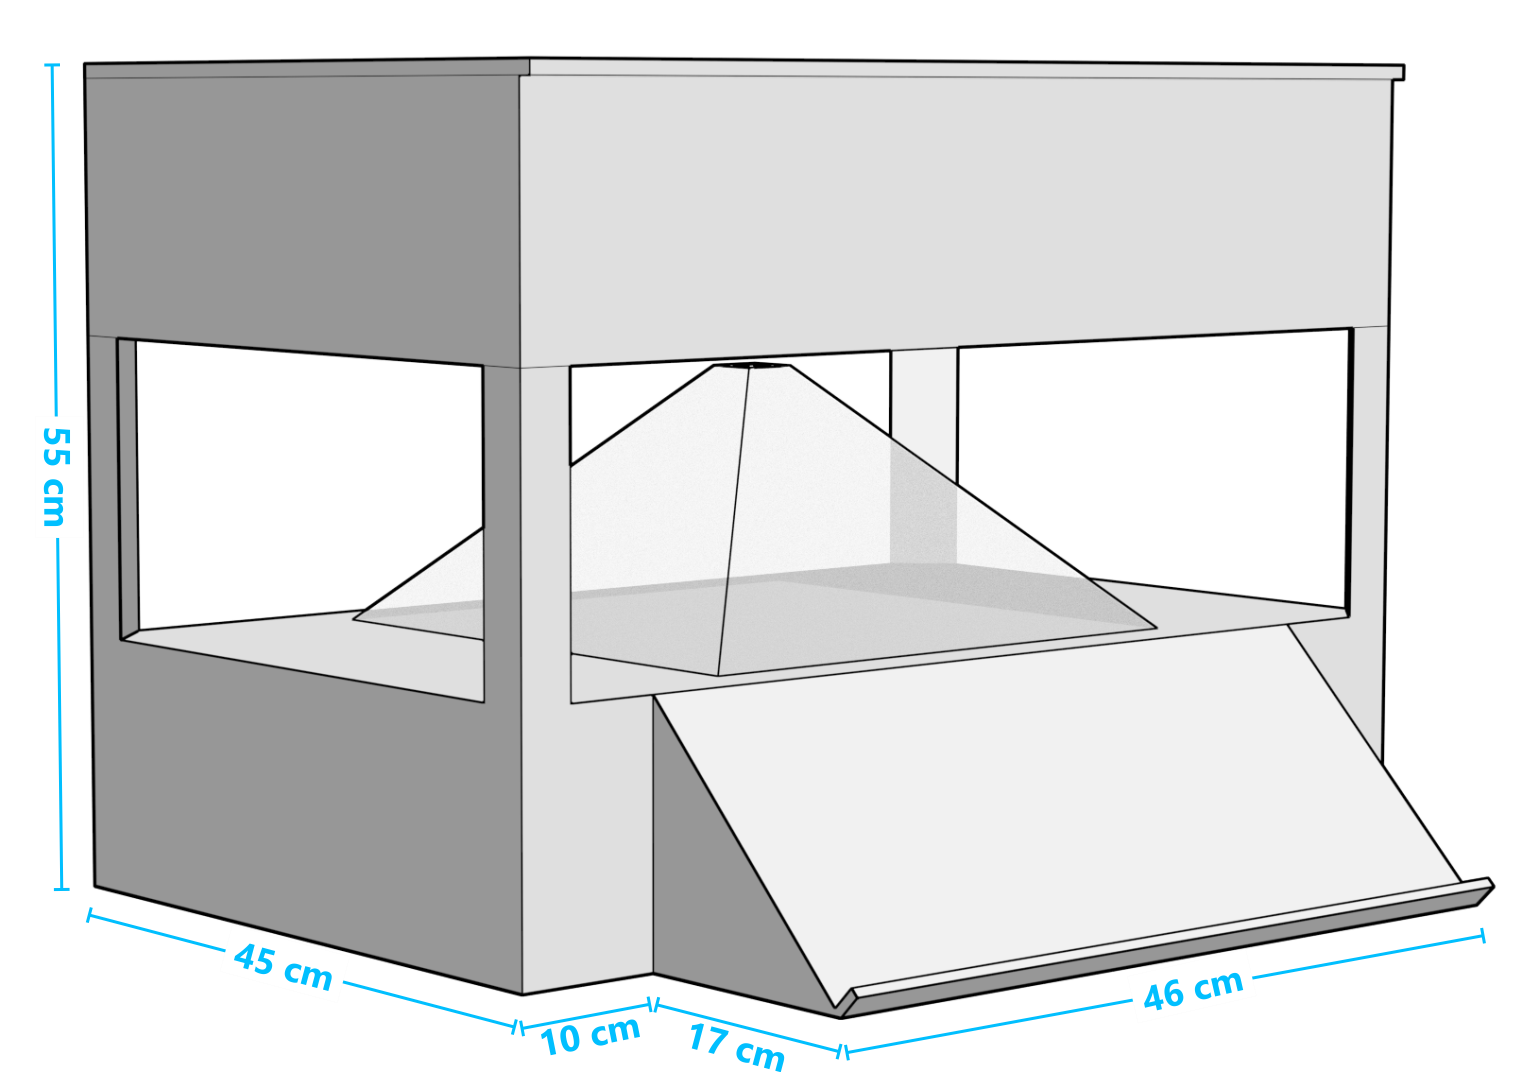
\includegraphics[width=0.75\textwidth]{img/bab3/desain_perangkat.png}
			\caption{Desain setting perangkat.}
			\label{fig:desain_setting}
		\end{figure}
		\vspace{-2ex}
		Penjelasan detail dari set yang dirancang dijelaskan melalui gambar \ref{fig:desain_setting}. Setting perangkat ini terdiri dari 3 bagian utama. Pada bagian atas, semua sisi tertutup kecuali sisi penompang \textit{display monitor} yang dilapisi dengan spons busa untuk menghindari kerusakan pada layar monitor. Di sisi berlawanannya dapat dibuka dan ditutup untuk memindahkan \textit{display monitor} dari set. Pada bagian tengah dibangun oleh penyangga di setiap sudut, dimana salah satunya menjadi jalur pengkabelan. \textit{Pyramid hologram} diposisikan di sisi tengah pada bagian ini dengan sisi terkecilnya menghadap \textit{display monitor}. \textit{Pyramid hologram} ini akan memantulkan \textit{hologram video} tepat pada bagian dalam. Leap Motion diletakkan pada sisi depan set yang terdapat sisi miring yang juga menompang \textit{information monitor}. Semua pengkabelan dari \textit{display monitor}, Leap Motion, serta \textit{information monitor} berpusat di bagian bawah set yang kemudian keluar melalui sisi belakang untuk disambungkan dengan \textit{server computer} beserta sumber listrik. Untuk menghindari adanya pantulan cahaya yang dapat mengganggu objek hologram yang dibentuk, setting perangkat dilapisi dengan stiker hitam polos di setiap sisi bagiannya.
	\vspace{1ex}
	
		\subsubsection{Desain \textit{Pyramid Hologram}}
		\vspace{0.5ex}
			Perancangan \textit{pyramid hologram} diperlukan agar hologram yang direfleksikan dapat tervisualisasikan dengan ukuran yang sesuai harapan. Prinsip kerja dari \textit{pyramid hologram} ini ditampilkan melalui gambar \ref{fig:prinsip_piramid}. Pada penelitian ini, jenis \textit{pyramid hologram} yang digunakan yaitu dengan piramid 4 sisi yang menghasilkan 4 objek jatuh di tengah-tengah piramid. Berdasarkan hal tersebut maka membutuhkan 4 buah segitiga sama kaki yang membentuk piramid dengan alas berbentuk persegi yang ukuran maksimalnya sebesar lebar monitor ($\ell$) yang digunakan dengan tinggi piramida sebesar setengah lebar monitor($\frac{1}{2}\ell$) membentuk sudut 45° antara sisi segitiga dengan \textit{display monitor}. Pemotongan pucuk piramida yang digunakan pada penelitian ini adalah sebesar sepersepuluh dari alas piramida.
			\begin{figure} [H]
				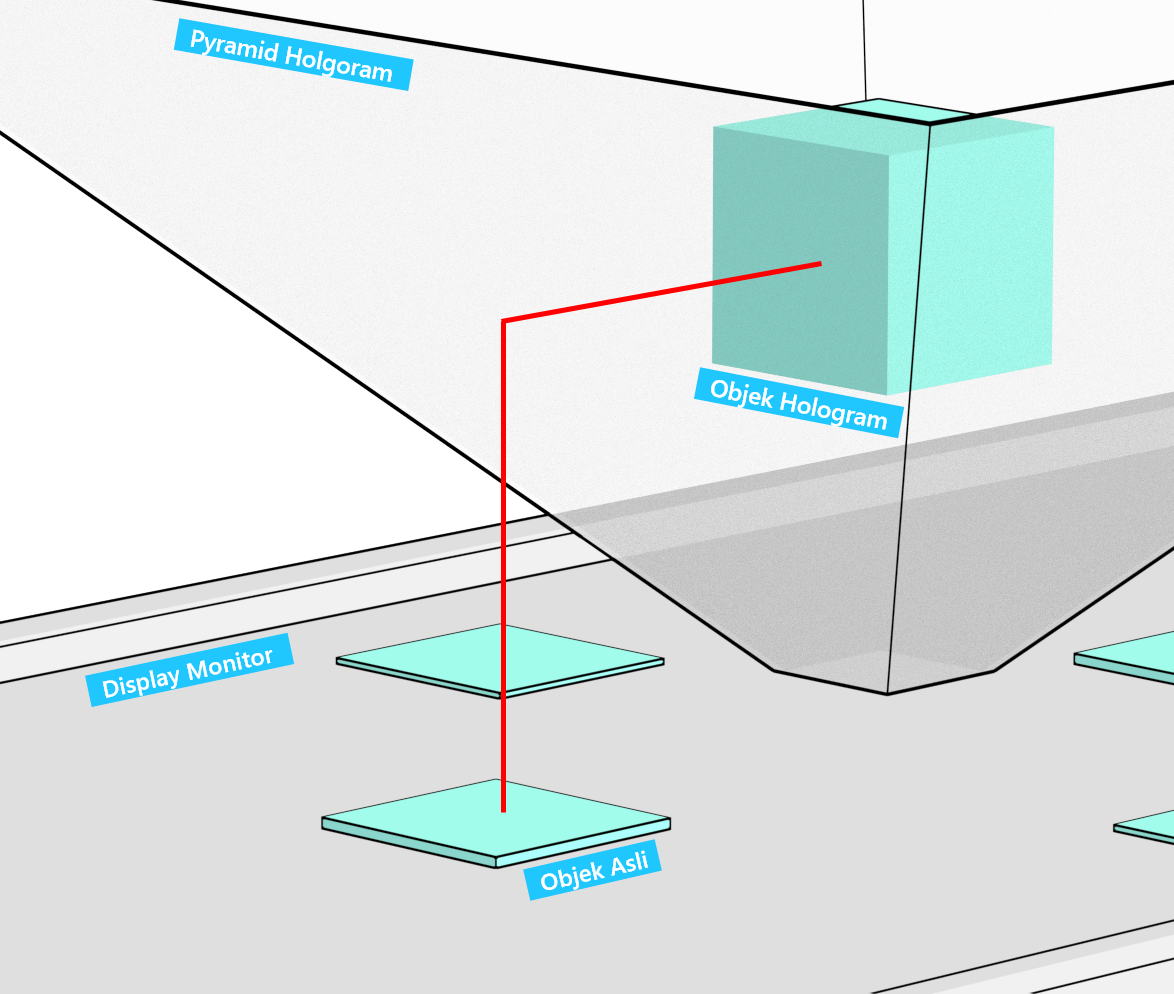
\includegraphics[width=0.6\textwidth]{img/bab3/prinsip_piramid.png}
				\caption{Prinsip \textit{pyramid hologram}.}
				\label{fig:prinsip_piramid}
			\end{figure}
			\vspace{-2ex}
			
			\begin{figure} [H]
				\subfloat[Perbandingan piramida dan objek hologram. \label{fig:piramida4}]{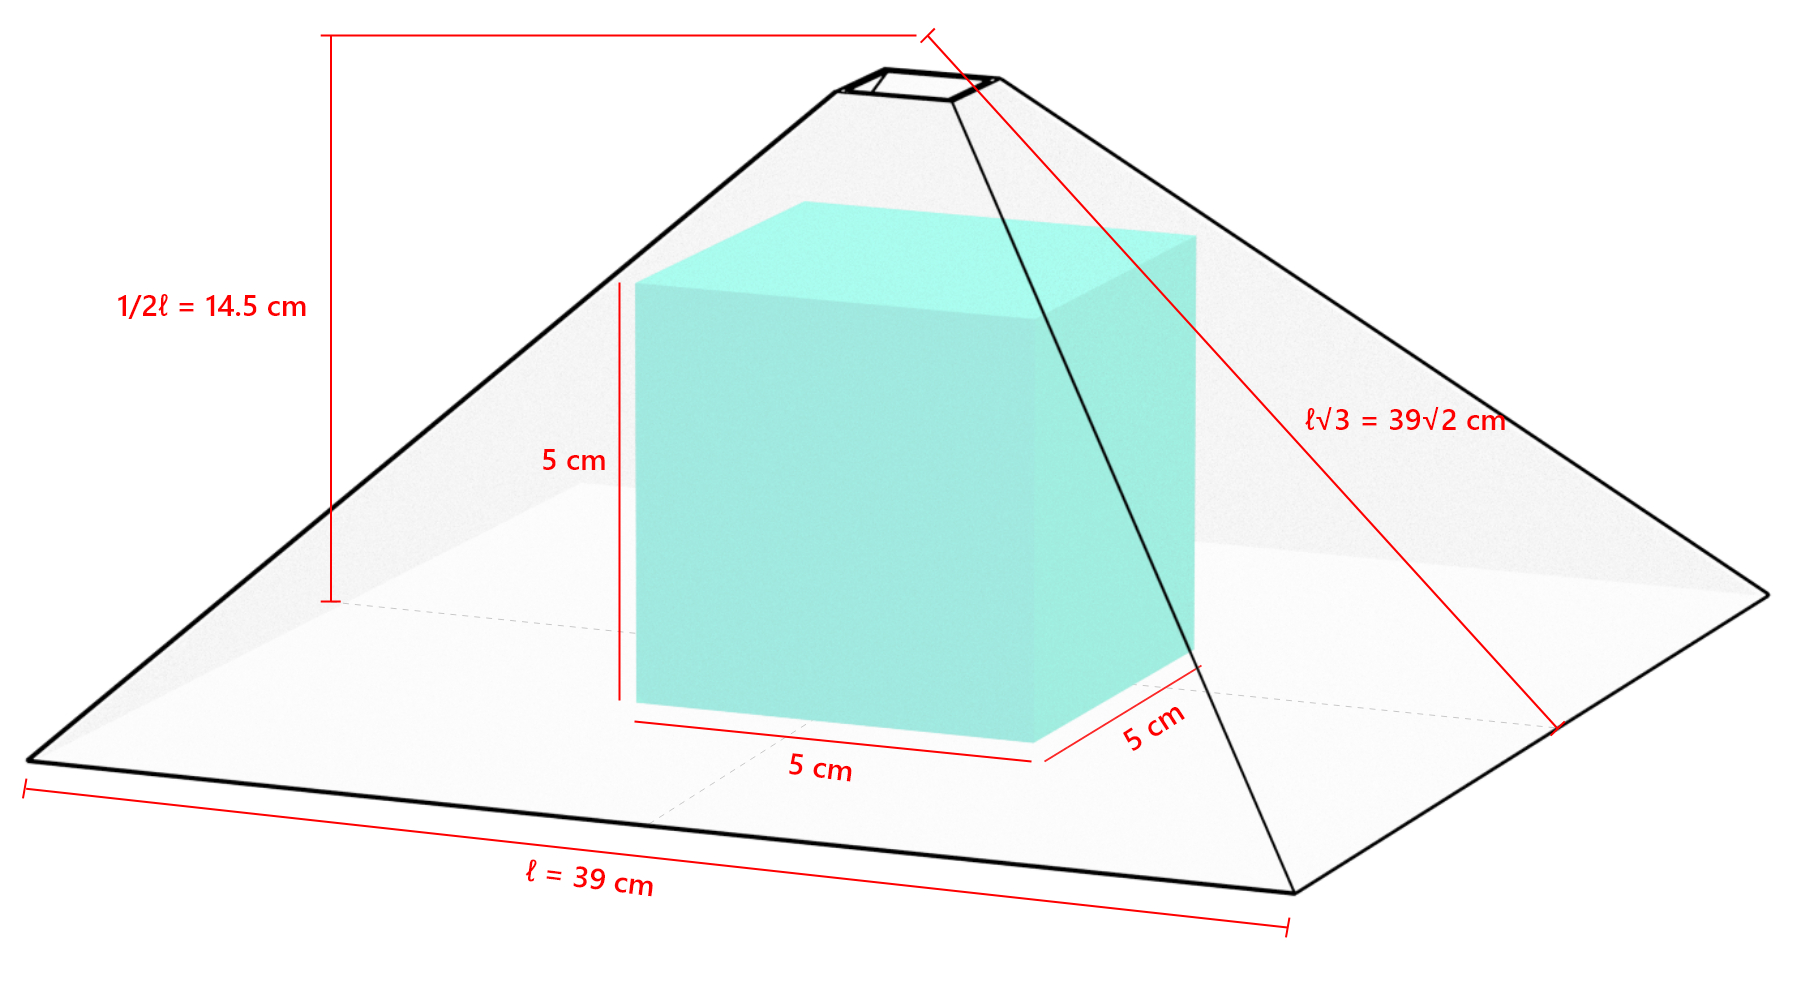
\includegraphics[width=0.85\textwidth]{img/bab3/piramida4.png}}
				\hspace{0.1em}
				\subfloat[Segitiga piramida awal. \label{fig:piramida2}]{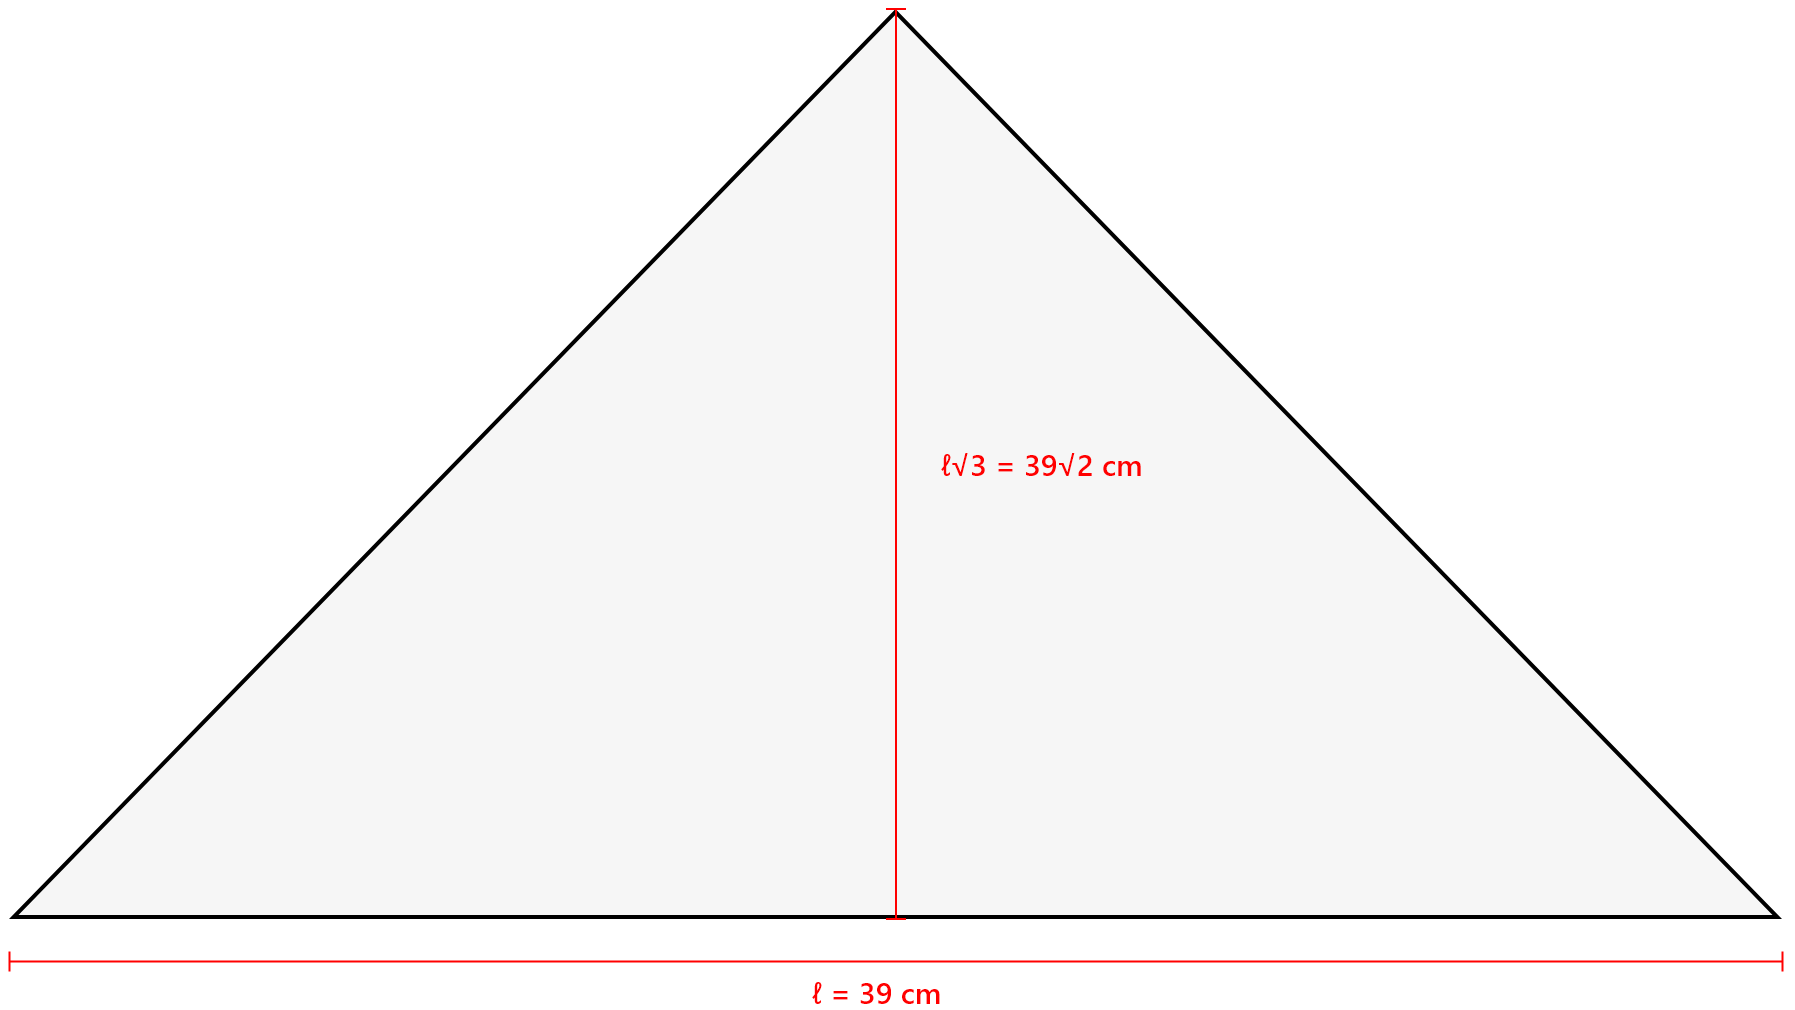
\includegraphics[width=0.55\textwidth]{img/bab3/piramida2.png}}
				\hspace{0.1em}
				\subfloat[Segitiga piramida akhir. \label{fig:piramida3}]{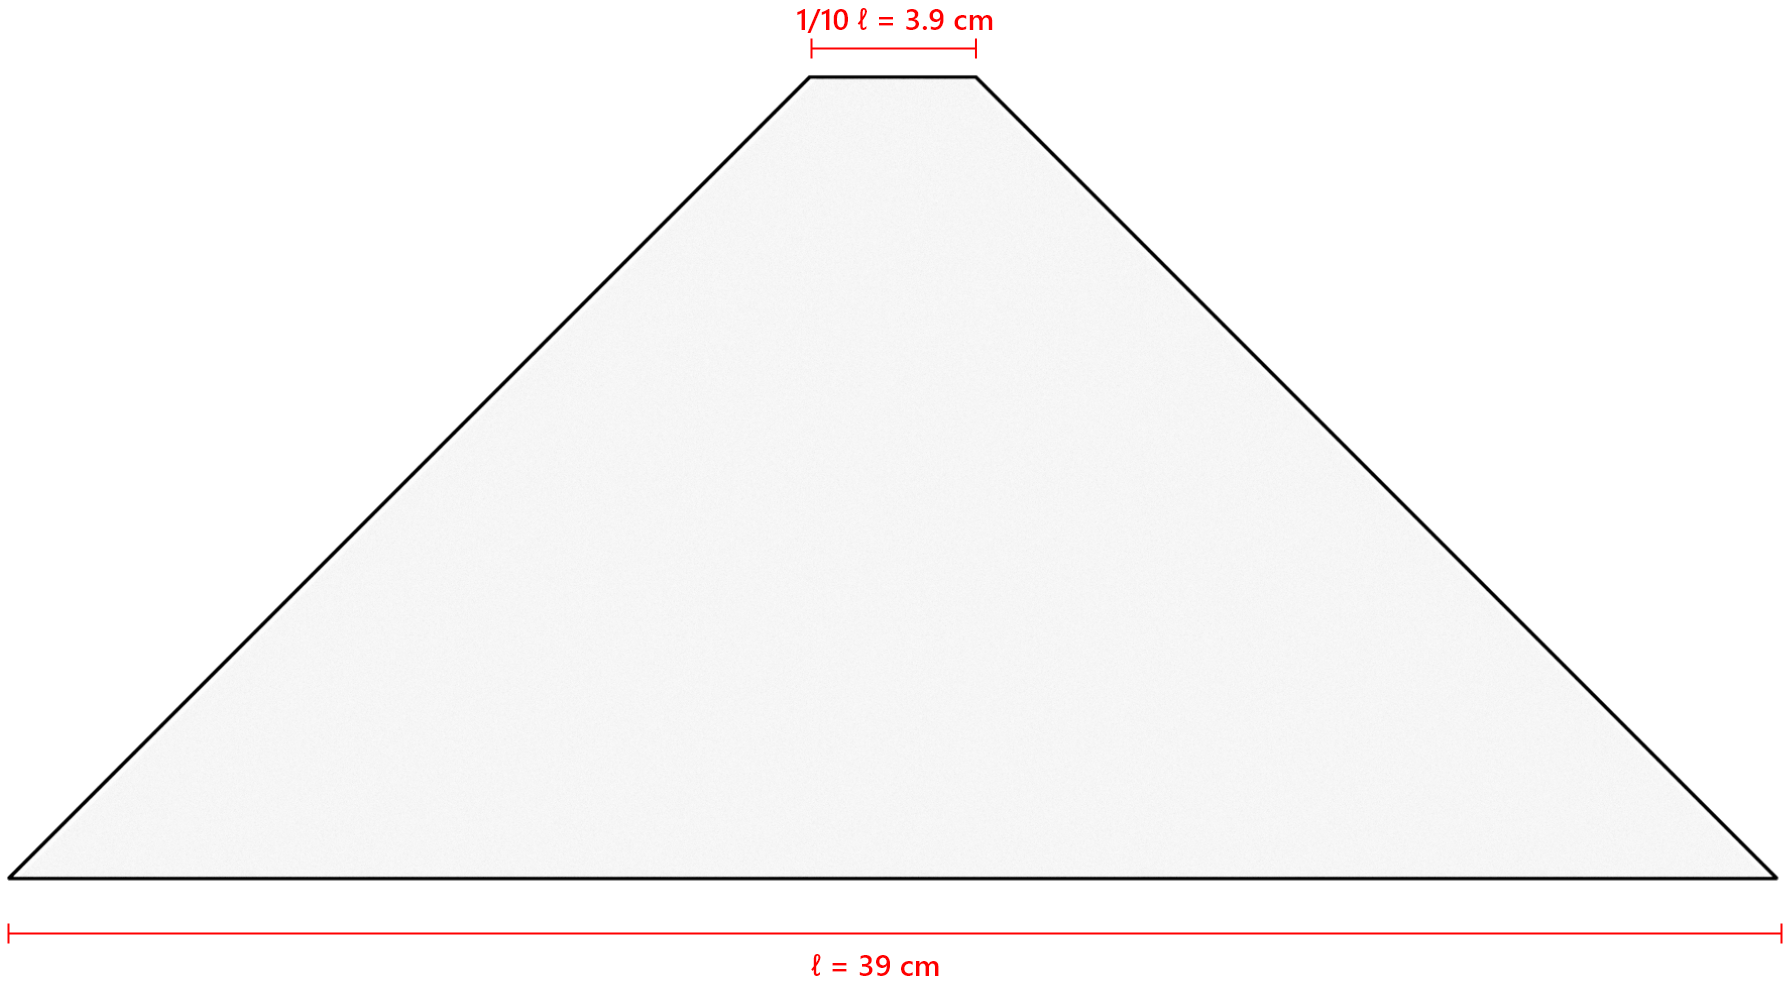
\includegraphics[width=0.55\textwidth]{img/bab3/piramida3.png}}
				\caption{Desain gestur yang membangun sistem interaksi.}
				\label{fig:desainpiramida}
			\end{figure}
			\vspace{-2ex}
		
			Sehingga desain \textit{pyramid hologram} yang diterapkan pada penelitian ini ditunjukkan melalui gambar \ref{fig:desainpiramida}. Dengan alas piramida berbentuk pesergi sebesar lebar monitor = 39 cm, maka tinggi piramida = 14.5 cm sesuai gambar \ref{fig:piramida4}. Kemudian untuk setiap sisi segitiganya memiliki alas = 39 cm dengan tinggi $39\sqrt{2}$ sesuai gambar \ref{fig:piramida2}. Terakhir, segitiga dipotong dengan sisi terpendeknya membentuk ukuran 3.9cm sesuai gambar \ref{fig:piramida3}. Dengan piramid seperti ini, maka besar objek hologram yang dapat diamati kurang dari 14.5 cm, idealnya adalah 5 x 5 x 5 cm sesuai gambar \ref{fig:piramida4} mendekati seperdelapan (7.8) dari lebar monitor yang digunakan. Bahan yang digunakan untuk membuat \textit{pyramid hologram} adalah akrilik ryben (hitam tembus pandang) yang berukuran 2 mm.
		%\vspace{0.75ex}
	\vspace{1.5ex}
	
	\subsection{Desain Sistem Visualisasi}
	\vspace{1ex}
		Sistem visualisasi yang diterapkan pada penelitian ini berkaitan dengan penyajian aplikasi di \textit{display} dan \textit{information monitor}. \textit{Display monitor} menampilkan \textit{hologram video}. \textit{Hologram video} akan terlihat sebagai bentuk objek hologram karena adanya refleksi cahaya dari setiap sisi \textit{pyramid hologram}. Sedangkan \textit{information monitor} menampilkan informasi dan \textit{interface} aplikasi. \textit{Information monitor} juga menerima inputan dari pengguna untuk mengatur aplikasi melalui tombol yang disediakan. Alur kerja dari sistem visualisasi yang diterapkan ditunjukkan pada gambar \ref{fig:desain_visualisasi}.
		\begin{figure} [H]
			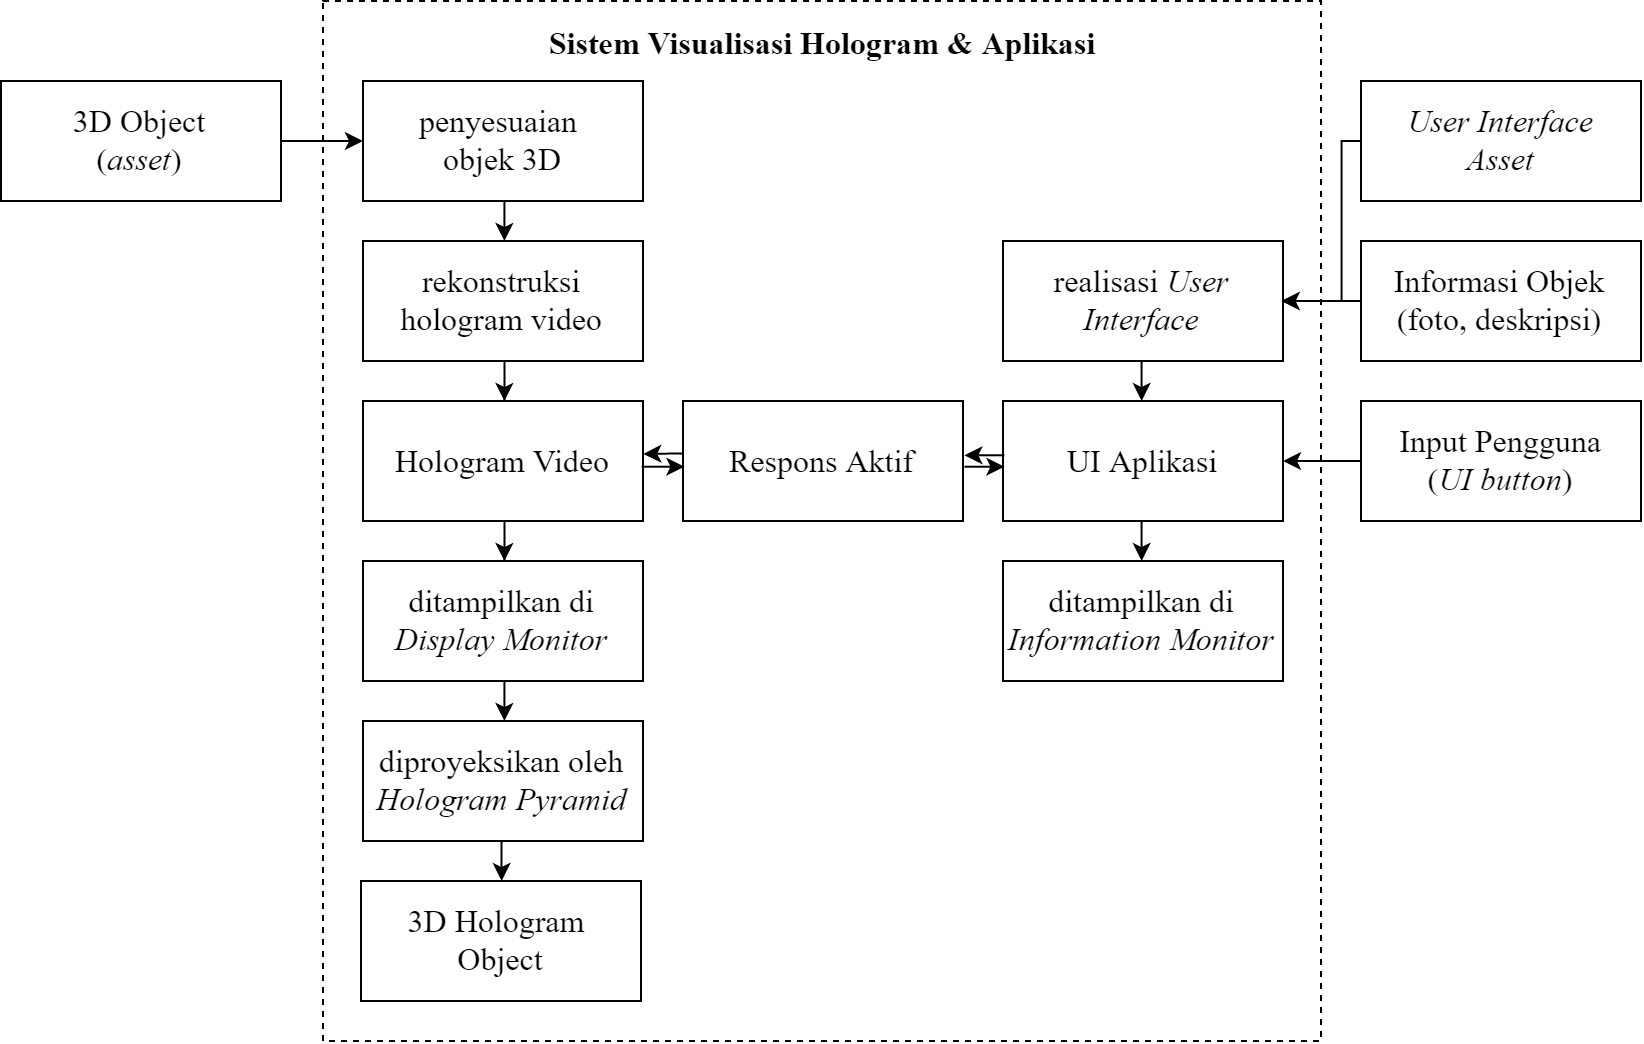
\includegraphics[width=\textwidth]{img/bab3/desain_visualisasi.png}
			\caption{Alur kerja sistem visualisasi.}
			\label{fig:desain_visualisasi}
		\end{figure}
		\vspace{-2ex}
		
		Tampilan utama kedua monitor saat permainan dimulai ditunjukkan pada gambar \ref{fig:desain_monitor}. Hologram video pada \textit{display monitor} menampilkan 4 sisi objek yang ketika diproyeksikan menghasilkan objek hologram sesuai dengan gambar \ref{fig:proyeksihologram}. Penempatan informasi objek pada \textit{information monitor} ditunjukkan pada gambar \ref{fig:desain_im}.
		
		Selain menampilkan informasi objek, \textit{information monitor} juga menampilkan \textit{user interface} aplikasi. Aplikasi terbagi menjadi dua bagian utama yang ditunjukkan pada gambar \ref{fig:storyboard}. \textit{Main Menu} atau Menu Utama merupakan tampilan awal saat aplikasi tersebut dijalankan. Bagian ini terdiri dari beberapa pilihan menu yang dapat diakses oleh pengguna, di antaranya \textit{How to Play} untuk menunjukkan cara penggunaan perangkat, \textit{About} untuk menunjukkan informasi mengenai produk dan developer, dan \textit{Exit} untuk keluar dari permainan. Sedangkan opsi \textit{Start} yang akan memulai bagian \textit{Main Scene} berupa \textit{scene} utama atau \textit{gameplay}.
		\vspace{-2ex}
		\begin{figure} [H]
			\subfloat[Tampilan \textit{Display Monitor}. \label{fig:desain_dm}]{
\includegraphics[width=0.6\textwidth]{img/bab3/desain_dm.png}}
			\hspace{0.1em}
			\subfloat[Tampilan \textit{Information Monitor}. \label{fig:desain_im}]{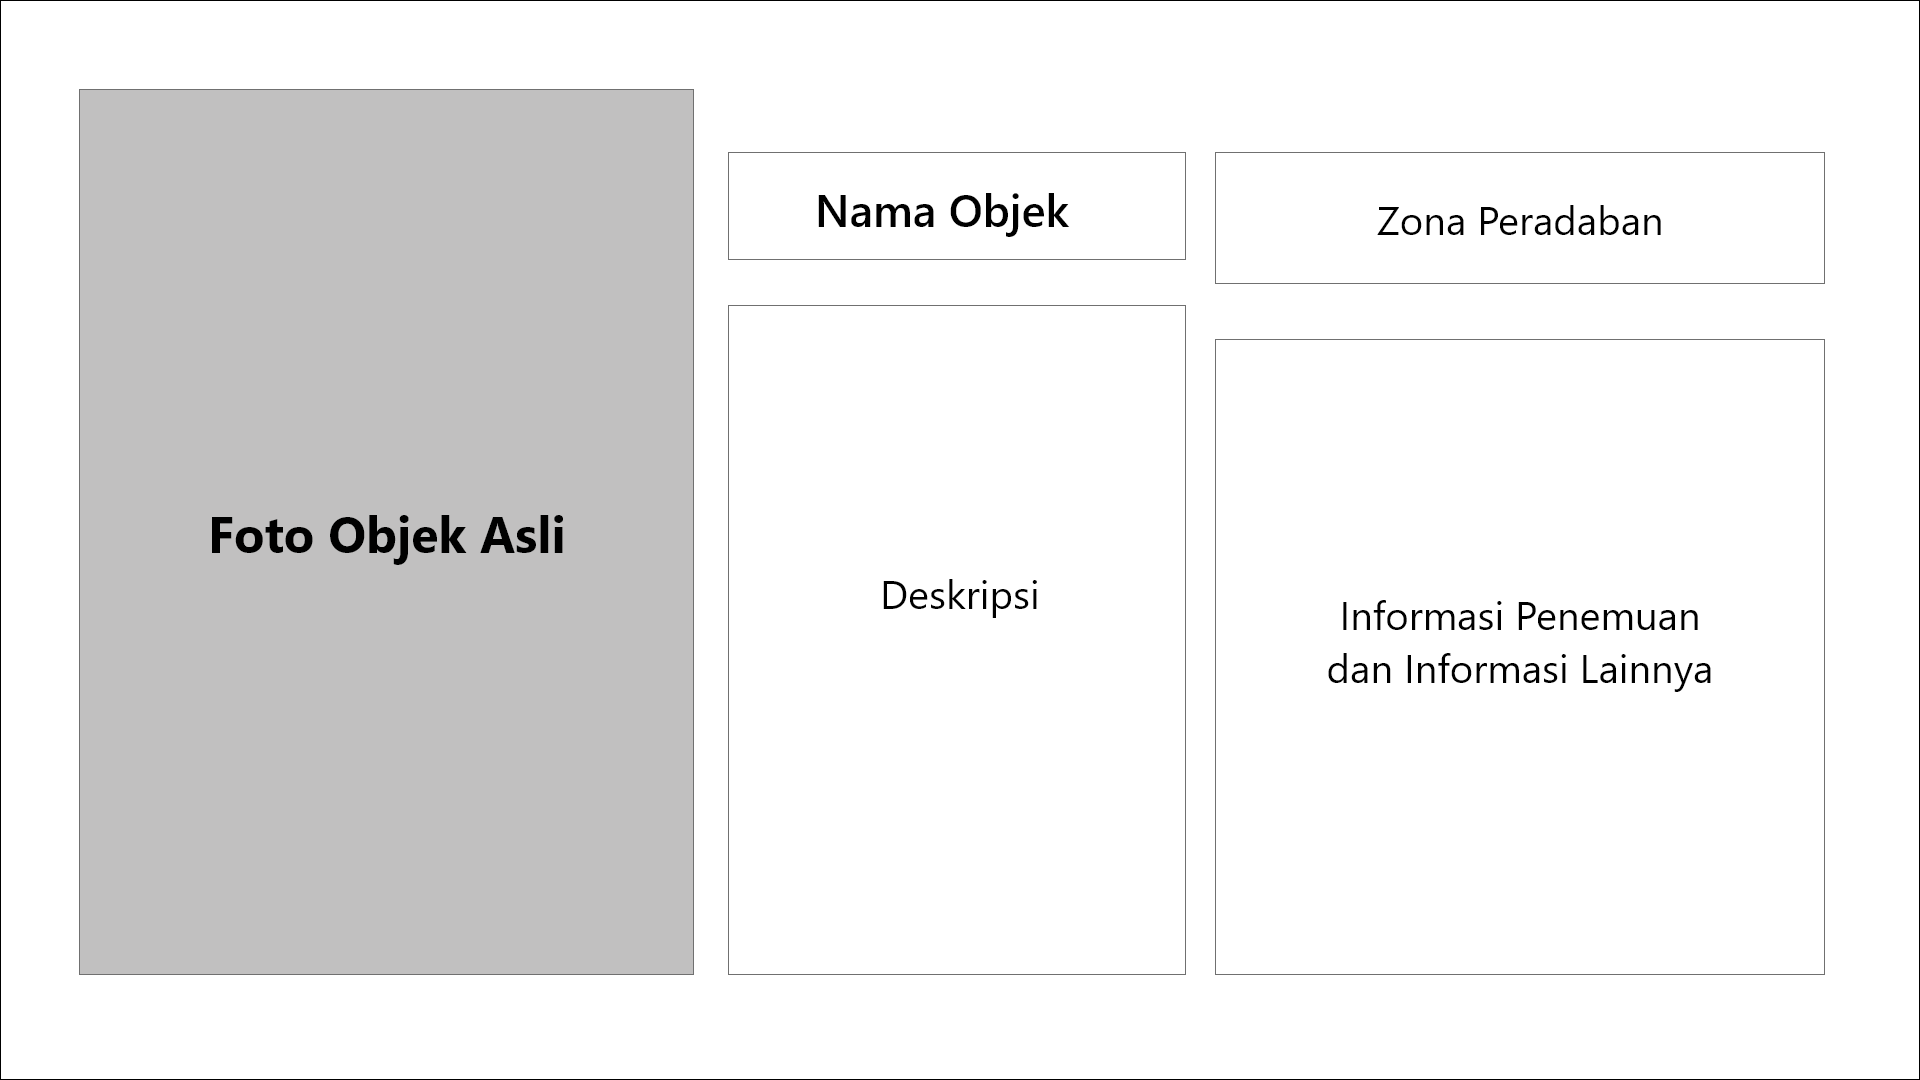
\includegraphics[width=0.6\textwidth]{img/bab3/desain_im.png}}
			\caption{Tampilan utama kedua monitor sistem visualisasi.}
			\label{fig:desain_monitor}
		\end{figure}
		\vspace{-2ex}
		\begin{figure}[H]
			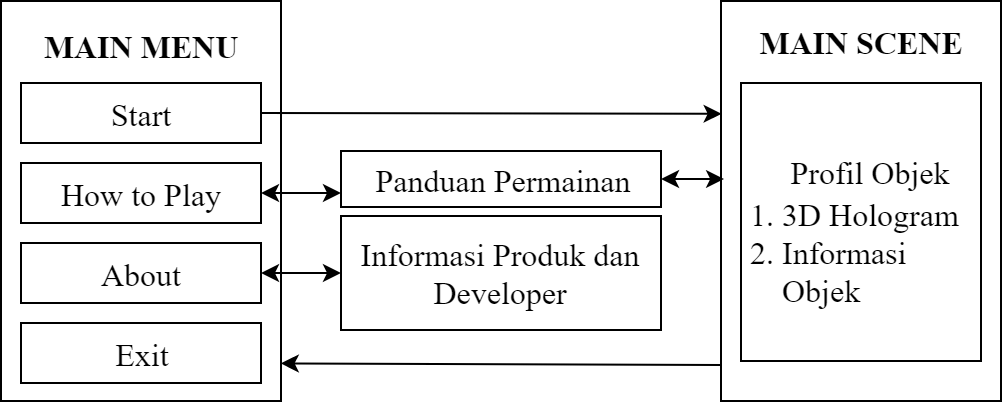
\includegraphics[width=0.8\textwidth]{img/bab3/storyboard.png}
			\caption{Desain alur menu aplikasi.}
			\label{fig:storyboard}
		\end{figure}
		\vspace{-2ex}
		\begin{figure}[H]
			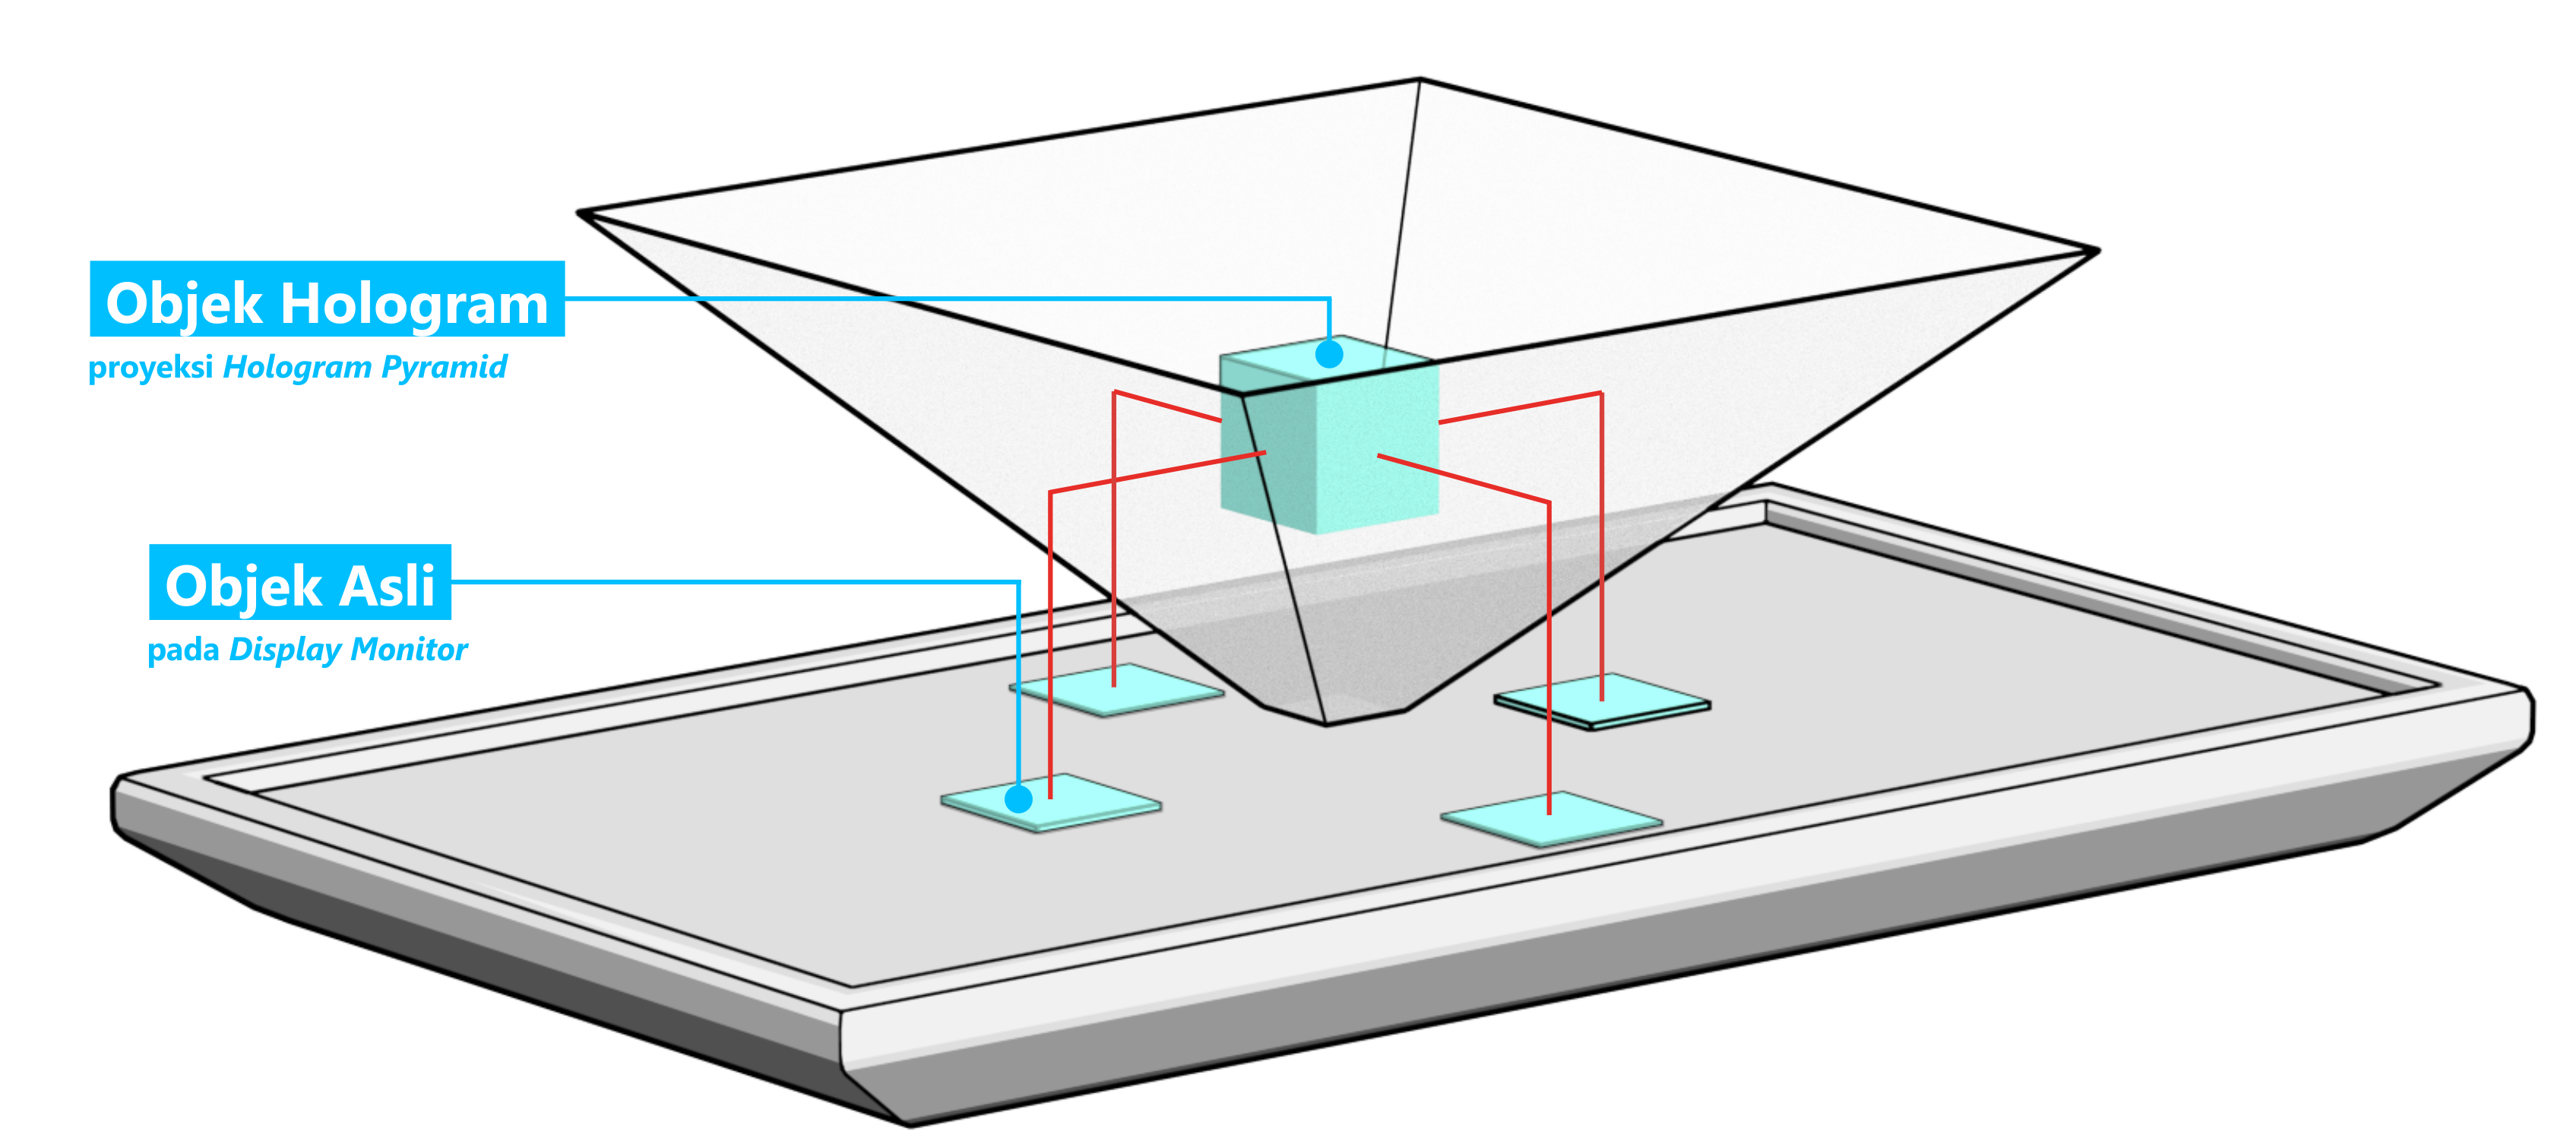
\includegraphics[width=\textwidth]{img/bab3/mekanismehologram.png}
			\caption{Mekanisme \textit{Display Monitor}.}
			\label{fig:proyeksihologram}
		\end{figure}
	\vspace{1.5ex}
	
	\subsection{Desain Sistem Interaksi}
	\vspace{1ex}
		Sistem interaksi yang diterapkan pada penelitian ini menggunakan Leap Motion untuk menangkap \textit{hand gesture} yang diberikan oleh pengguna terhadap objek hologram. Leap Motion bekerja dengan cara mendeteksi adanya pergerakan tangan di dalam jangkauan area pandangnya, kemudian mengirimkan data tersebut ke komputer server untuk diolah dan diambil informasi yang dibutuhkan. Ketika hasil yang diperoleh sesuai dengan fitur yang dibangun, kemudian mengaktifkan respons yang selanjutnya ditunjukkan oleh objek 3D. Alur kerja dari sistem interaksi yang diterapkan ditunjukkan pada gambar \ref{fig:desain_interaksi}.
		\begin{figure} [H]
			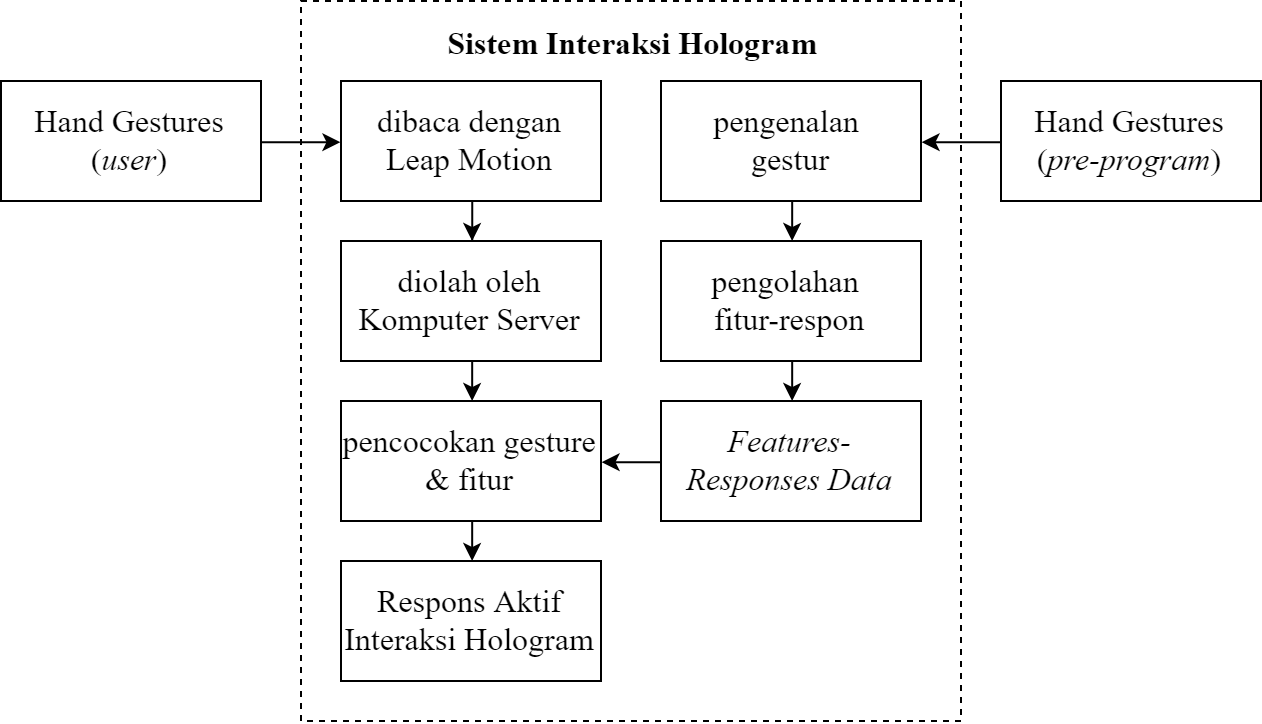
\includegraphics[width=\textwidth]{img/bab3/desain_interaksi.png}
			\caption{Alur kerja sistem interaksi.}
			\label{fig:desain_interaksi}
		\end{figure}
		\vspace{-2ex}
	
		Interaksi yang dapat dilakukan oleh pengguna terhadap sistem visualisasi yang dibangun di antaranya adalah mengeksplorasi objek hologram dan menampilkan menu yang bersesuaian. Fitur-respons yang disediakan berdasarkan \textit{hand gesture} ini ditunjukkan melalui gambar \ref{fig:storyboardgestur}. Semua gestur yang dibangun memiliki ketentuan yang berbeda dalam mengaktifkan respons terkait. Khusus gestur cubitan atau \textit{pinch} untuk mengeksplorasi objek (gambar \ref{fig:gestur2}), gestur \textit{high five} untuk \textit{reset} objek (gambar \ref{fig:gestur4}), gestur \textit{upside} untuk menampilkan menu \textit{Help} (gambar \ref{fig:gestur6}), dan gestur \textit{home} untuk menampilkan \textit{Main Menu} atau keluar dari \textit{Main Scene} (gambar \ref{fig:gestur7}), respons hanya terpanggil jika gestur terdeteksi di kedua tangan secara bersamaan. 
		
		Namun tidak semua gestur membutuhkan kedua tangan (kanan dan kiri) untuk mengaktifkan respons yang bersesuaian. Gestur tersebut di antaranya yaitu gestur genggam atau \textit{punch} (gambar \ref{fig:gestur1}) untuk mengeskplorasi objek, gestur tembak atau \textit{gun} (gambar \ref{fig:gestur3}) untuk mengaktifkan animasi objek, gestur \textit{side thumb} (gambar \ref{fig:gestur5}) untuk mengganti objek yang ditampilkan, dan gestur \textit{thumb up} (gambar \ref{fig:gestur8}) untuk membatalkan atau mengetujui pilihan. Keempatnya pun ada yang dapat mengaktifkan respons jika hanya ada satu gestur di salah satu tangan (kanan atau kiri). 
		
		Meskipun objek hologram dapat dilihat dari seluruh sisi setting perangkat, pengguna hanya dapat berinteraksi di salah satu sisi yang telah dilengkapi dengan \textit{information monitor} dan Leap Motion.
		
		\begin{comment}
		Pada akhirnya \textit{hand model} pada dunia virtual aplikasi akan dimatikan, sehingga menimbulkan kesan seolah-olah pengguna berinteraksi langsung dengan objek hologram dengan tangannya sendiri. 
		\end{comment}
		
		\vspace{-2ex}
		\begin{figure} [H]
			\subfloat[Gestur \textit{punch} untuk eksplorasi objek. \label{fig:gestur1}]{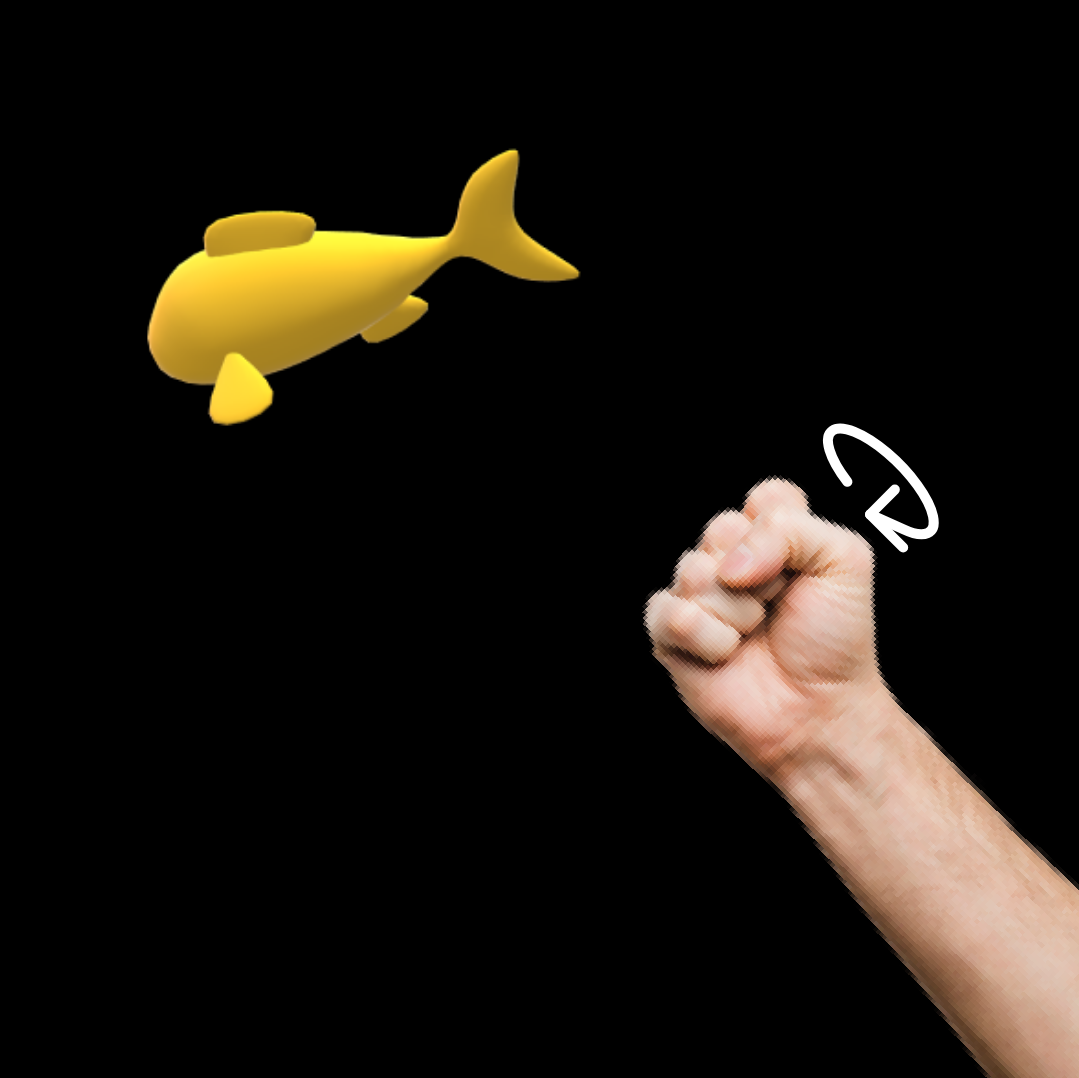
\includegraphics[width=0.32\textwidth]{img/bab3/gestur1.png}}
			\hspace{0.1em}
			\subfloat[Gestur \textit{pinch} untuk zoom objek. \label{fig:gestur2}]{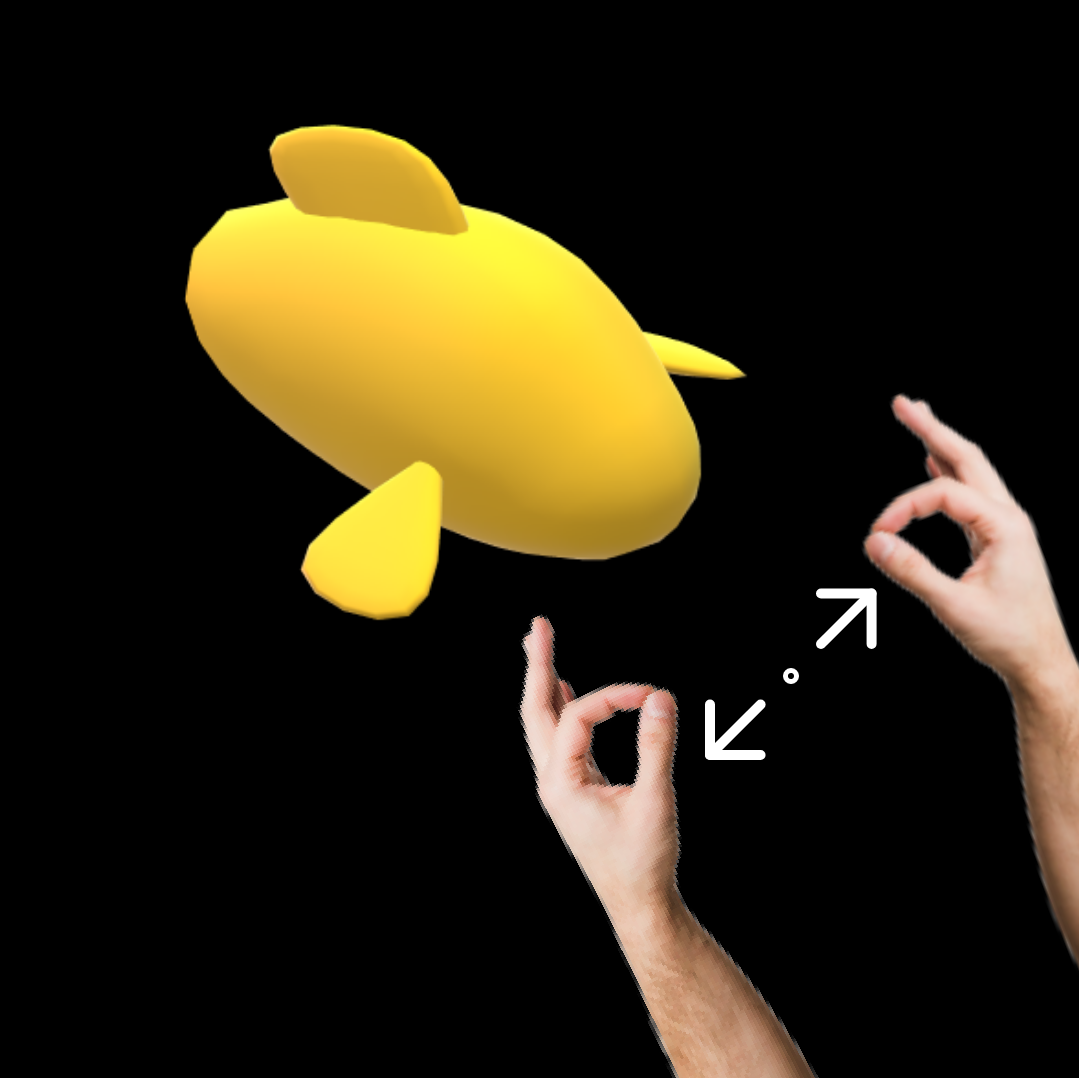
\includegraphics[width=0.32\textwidth]{img/bab3/gestur2.png}}
			\hspace{0.1em}
			\subfloat[Gestur \textit{gun} untuk mengaktifkan animasi. \label{fig:gestur3}]{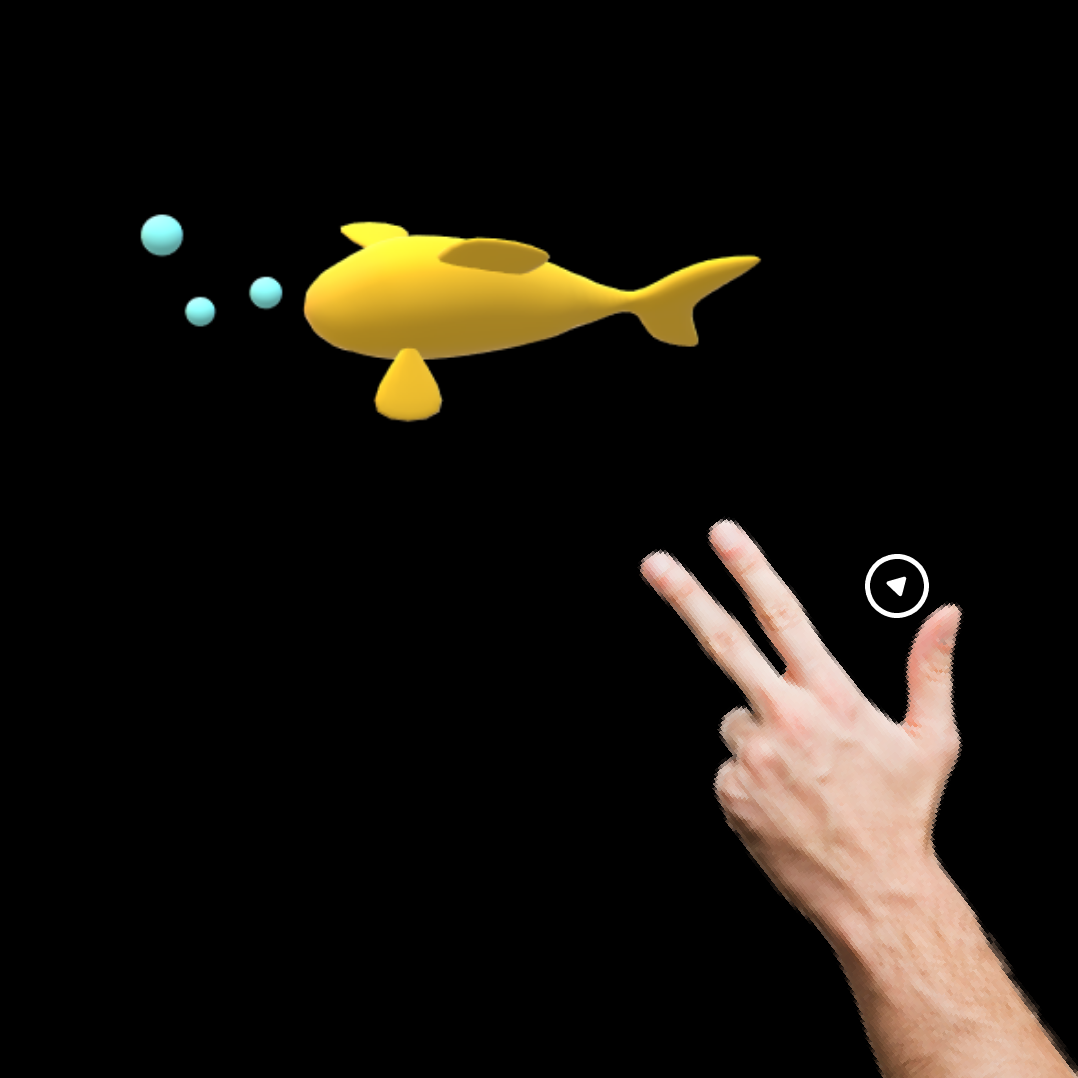
\includegraphics[width=0.32\textwidth]{img/bab3/gestur3.png}}
			\hspace{0.1em}
			\subfloat[Gestur \textit{high five} untuk \textit{reset} objek. \label{fig:gestur4}]{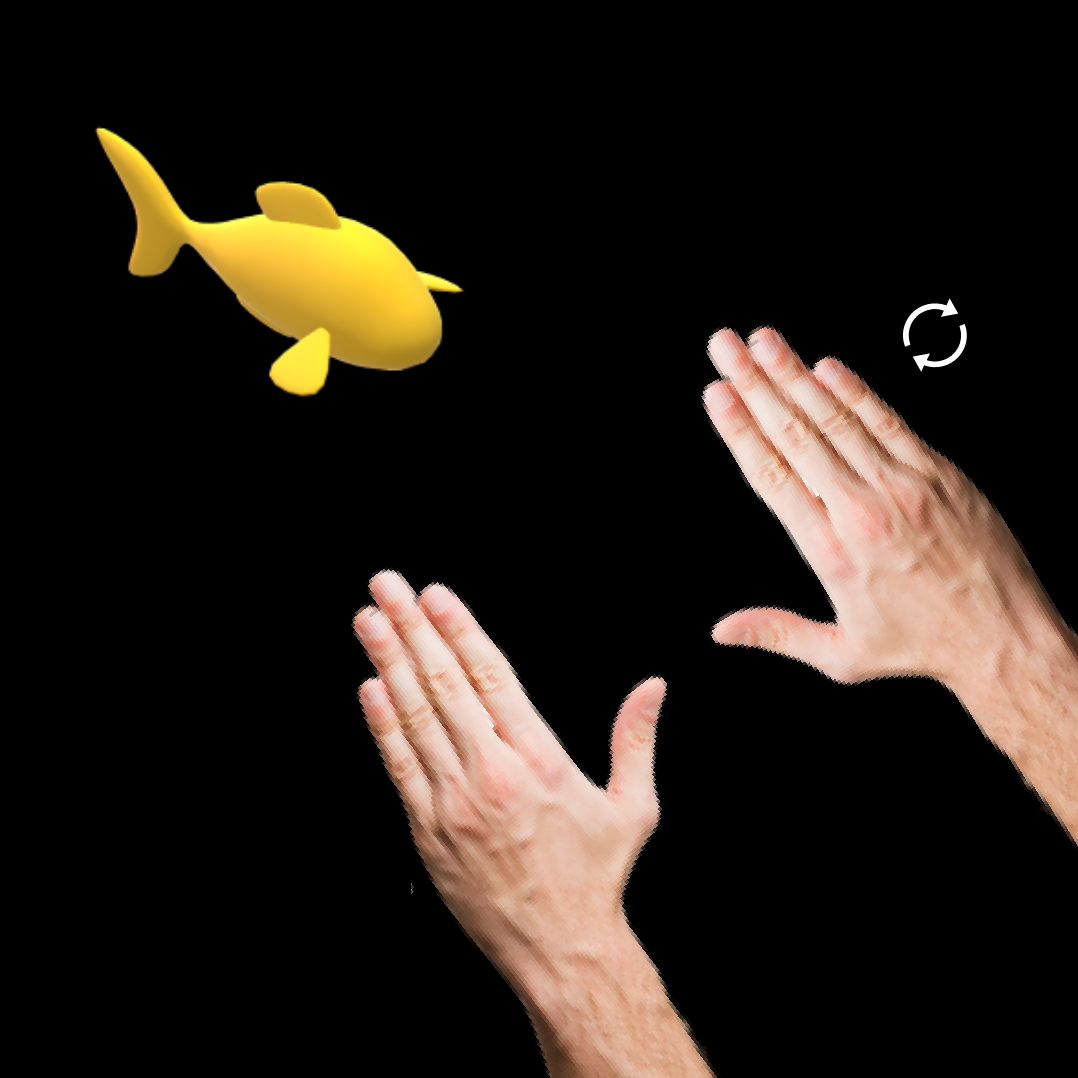
\includegraphics[width=0.32\textwidth]{img/bab3/gestur4.png}}
			\hspace{0.1em}
			\subfloat[Gestur \textit{thumb up} untuk ganti objek. \label{fig:gestur5}]{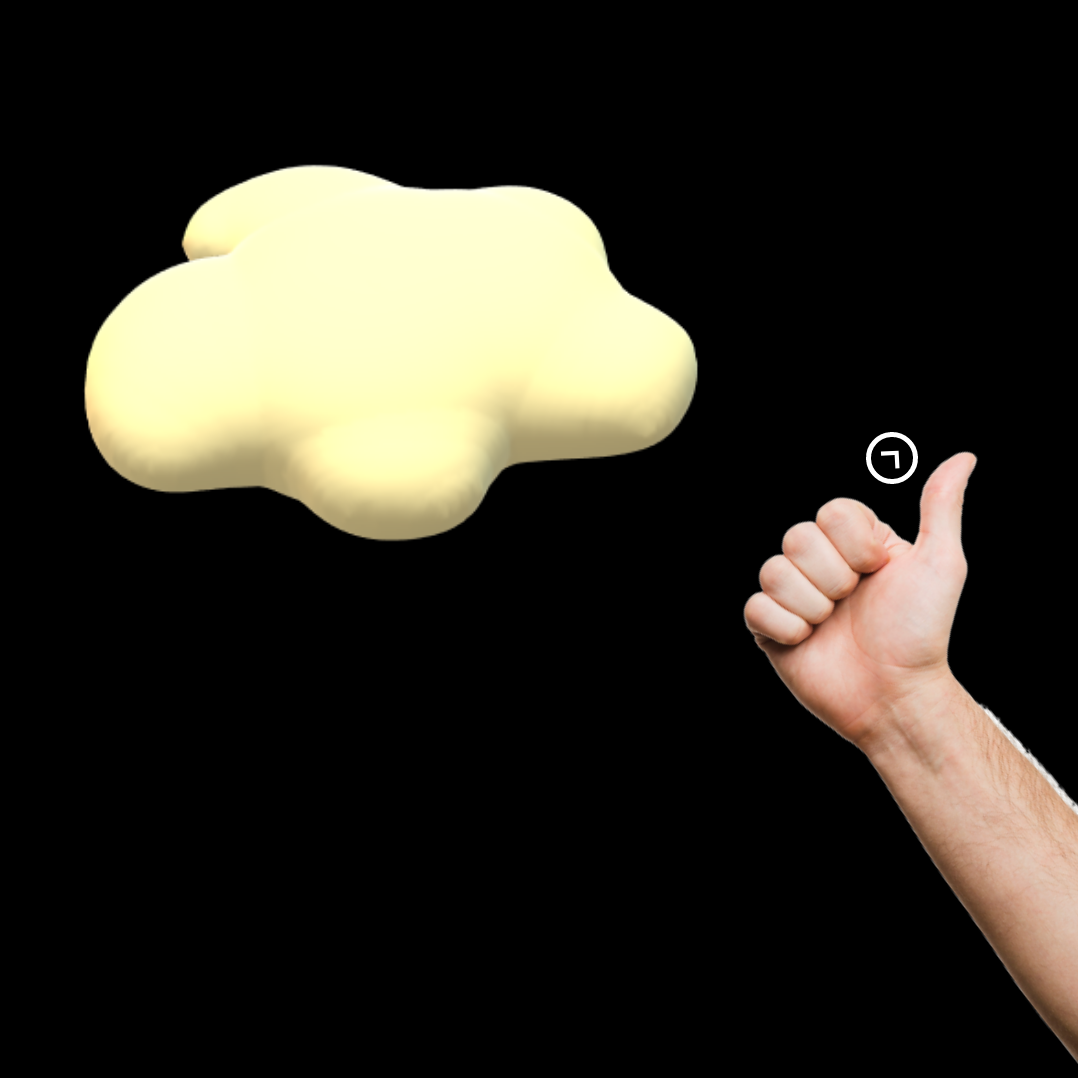
\includegraphics[width=0.32\textwidth]{img/bab3/gestur5.png}}
			\hspace{0.5em}
			\subfloat[Gestur \textit{upside} untuk menampilkan \textit{Help}.
			\label{fig:gestur6}]{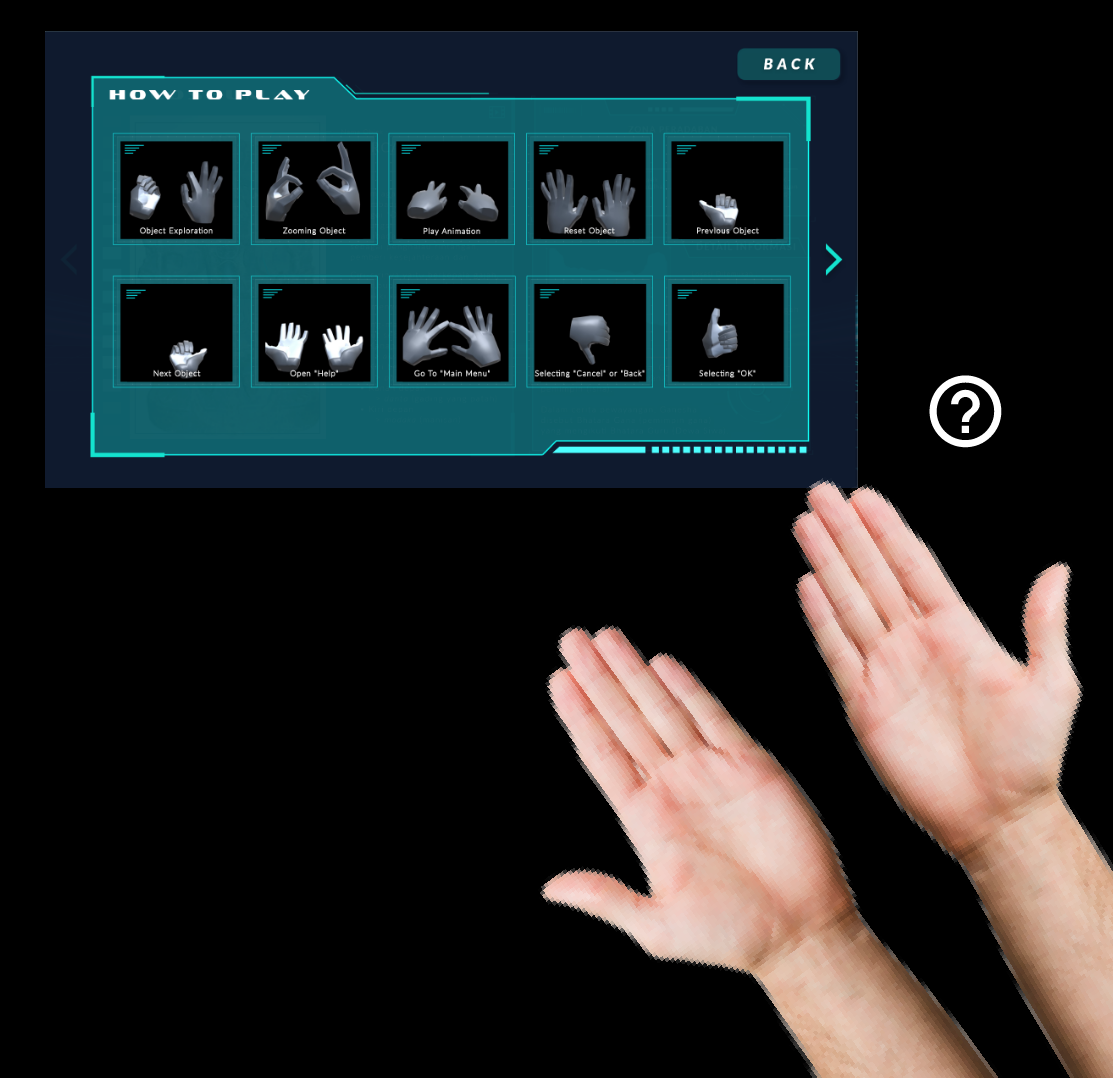
\includegraphics[width=0.32\textwidth]{img/bab3/gestur6.png}}
			\hspace{0.1em}
			\subfloat[Gestur \textit{home} untuk menampilkan \textit{Main Menu}.
			\label{fig:gestur7}]{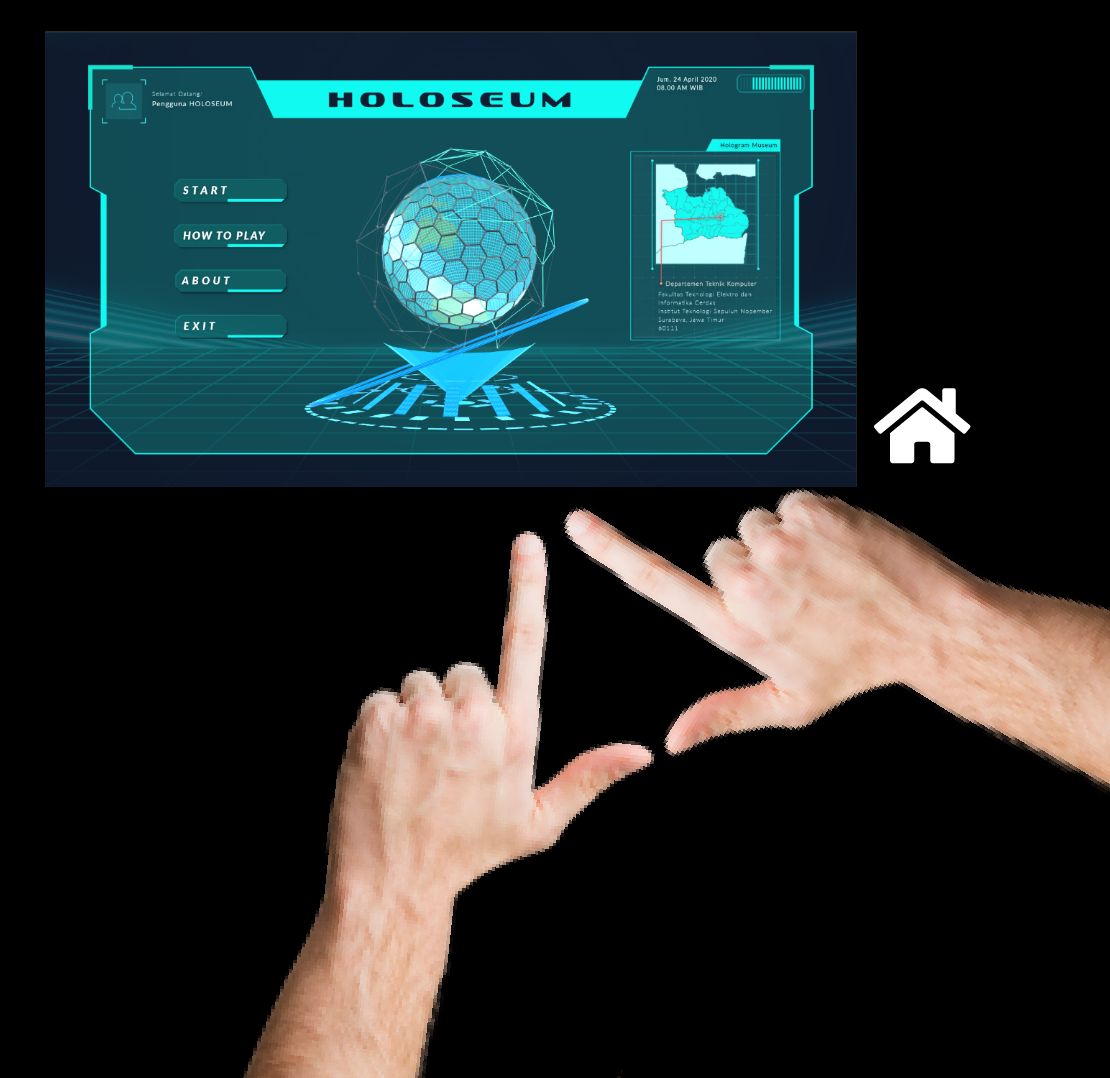
\includegraphics[width=0.32\textwidth]{img/bab3/gestur7.png}}
			\hspace{0.1em}
			\subfloat[Gestur \textit{thumb up} untuk membatalkan dan menyetujui pilihan.
			\label{fig:gestur8}]{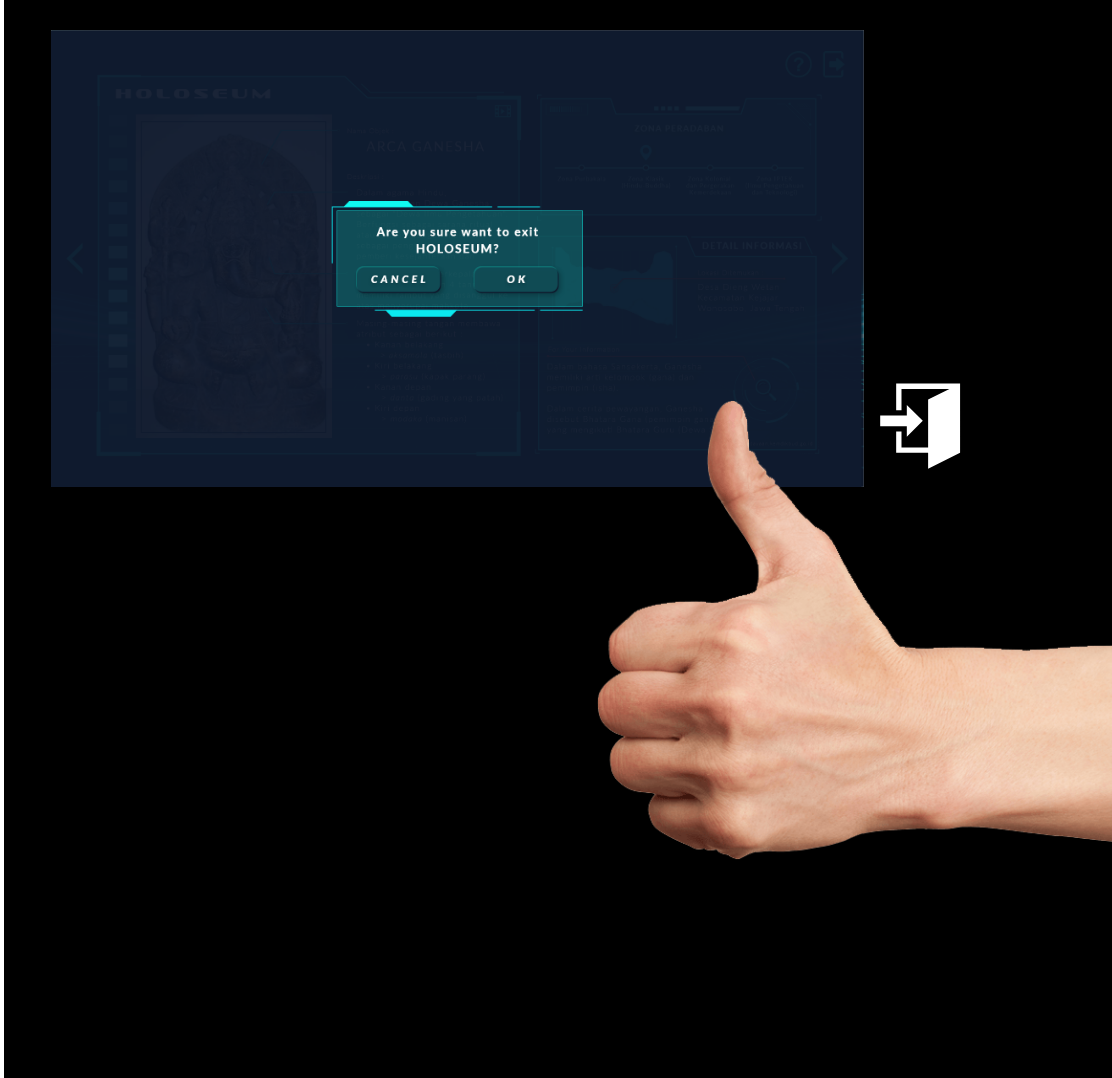
\includegraphics[width=0.32\textwidth]{img/bab3/gestur8.png}}
			\caption{Desain gestur yang membangun sistem interaksi.}
			\label{fig:storyboardgestur}
		\end{figure}
\vspace{2ex}

\section{Alur Implementasi Sistem}
\vspace{1ex}
	Alur implementasi dalam pengerjaan penelitian Tugas Akhir ini dapat dibagi menjadi beberapa tahapan sebagai penunjang dalam menjalankan penelitian.
	\begin{figure} [H]
		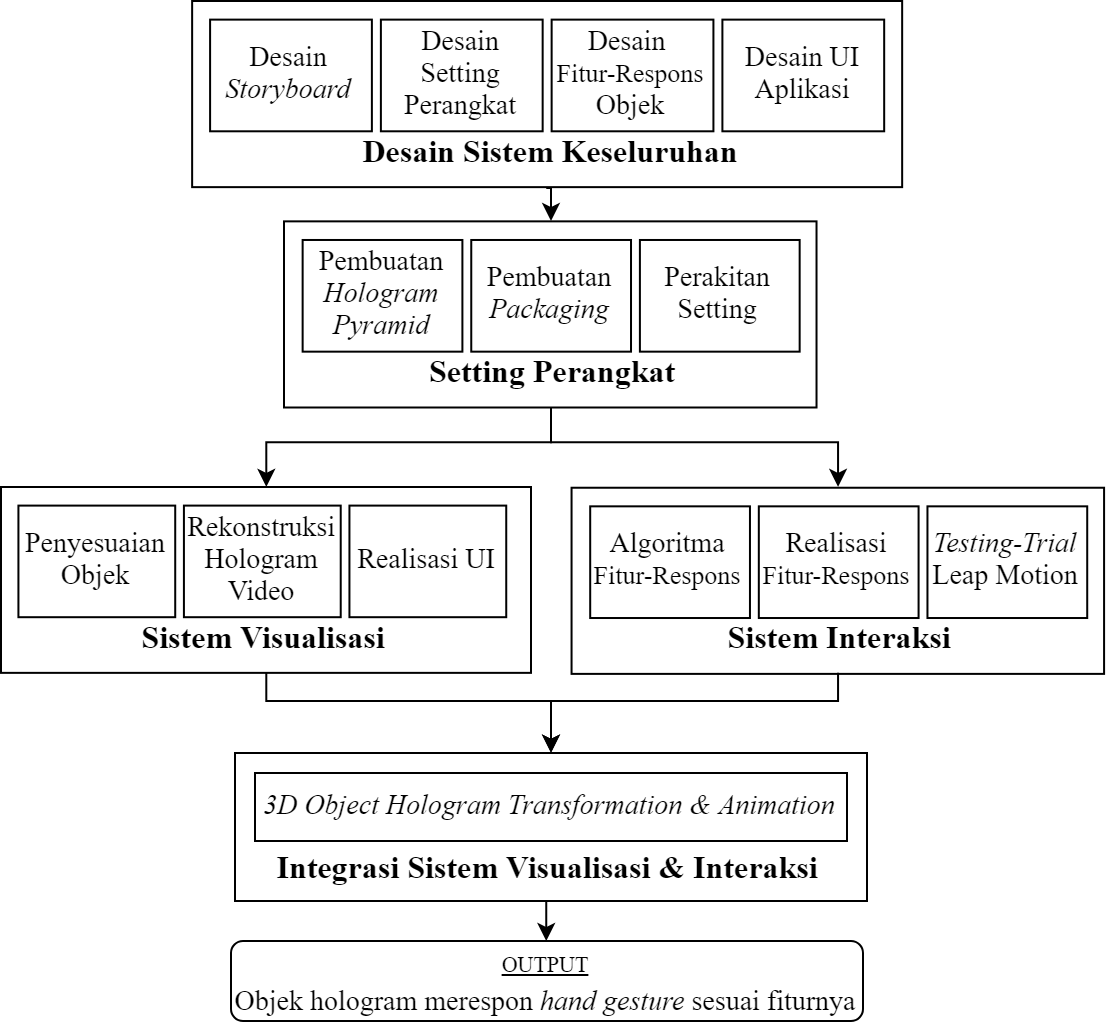
\includegraphics[width=\textwidth]{img/bab3/metodologi.png}
		\caption{Alur implementasi penelitian.}
		\label{fig:metodologi}
	\end{figure}

	Alur implementasi yang dilakukan dapat diuraikan secara sederhana pada gambar \ref{fig:metodologi} dan dapat dijelaskan sebagai berikut :
	\begin{enumerate} [nolistsep]
		\item \textbf{Desain Sistem Keseluruhan}.
		
		Perancangan ini berkaitan dengan keseluruhan sistem yang dibutuhkan, dari \textit{storyboard} penggunaan dan setting perangkat, visualisasi hologram 3D dan penampilan informasi, hingga interaksi antara pengguna dan objek hologram.
		
		\item \textbf{Pembuatan Sitem Visualisasi}.
		
		Pada tahap ini dilakukan pengumpulkan asset objek 3D yang dibutuhkan. Modifikasi dan penyesuaian objek 3D diperlukan agar siap diprogram dan ditampilkan dalam bentuk \textit{hologram video}. \textit{Interface} aplikasi juga direalisasikan di tahap ini.
		
		\item \textbf{Pembuatan Setting Perangkat}.
		
		\textit{Hologram video} yang dibuat diproyeksikan melalui \textit{pyramid hologram}. Berdasarkan desain yang direncanakan, maka dibuat dan disusun setting perangkatnya agar mampu menjalankan keseluruhan sistem.
		
		\item \textbf{Pembuatan Sistem Interaksi}.
		
		Objek hologram yang terbentuk dapat digerakkan oleh pengguna berdasarkan \textit{hand gesture} menggunakan Leap Motion. Untuk memahami \textit{hand gesture} yang diberikan, fitur tersebut dirancang dan direalisasikan pada tahap ini.
		
		\item \textbf{Integrasi Sistem Visualisasi dan Interaksi}.
		
		Pada tahap ini sistem visualisasi dan interaksi digabungkan pada set yang telah dirancang. Objek hologram yang ditampilkan dapat merespons gerakan pengguna sesuai dengan fitur yang diterapkan.
		
		\item \textbf{Pengujian Sistem}.
		
		Pengujian sistem dilakukan untuk mendapatkan hasil dari implementasi alat yang digunakan sebagai bahan evaluasi dan pengembangan selanjutnya. 
	\end{enumerate}
\vspace{2ex}
	


\section{Implementasi Setting Perangkat}
\vspace{1ex}
	Setting perangkat yang dirancang dibangun menggunakan bahan dasar multiplex (10mm dan 3mm). Setting perangkat yang direncanakan tidak dapat diselesaikan secara keseluruhan, hanya bagian penompang \textit{display monitor} saja yang berhasil dirakit. Akibat keadaan yang tidak stabil, pembuatan setting perangkat tidak dapat dilanjutkan. Maka dibentuklah setting sesuai yang ditampilkan pada gambar \ref{fig:foto_alat}. \textit{Server Computer} yang digunakan yaitu Asus ROG Strix GL553VD. \textit{Display monitor} yang digunakan adalah Acer X193HQ berukuran 18.5 inch (23 x 41 cm) dengan \textit{pyramid hologram} berukuran 24 x 24 x 12 cm berbahan akrilik transparan 2 mm. Peletakkan \textit{display monitor} dan \textit{pyramid hologram} ditukar sehingga \textit{display monitor} yang terletak di bawah menopang \textit{pyramid hologram} yang terbuka ke atas sesuai pada gambar \ref{fig:proyeksihologram}. Leap Motion diletakkan di depan salah satu sisi. Ukuran ideal dari objek hologram yang dapat ditampilkan adalah sebesar 3 x 3 x 3 cm (1/7.8 dari lebar monitor). Pengujian dilakukan sebagaimana yang akan diterapkan pada desain setting perangkat awal. 
	\begin{figure} [H]
		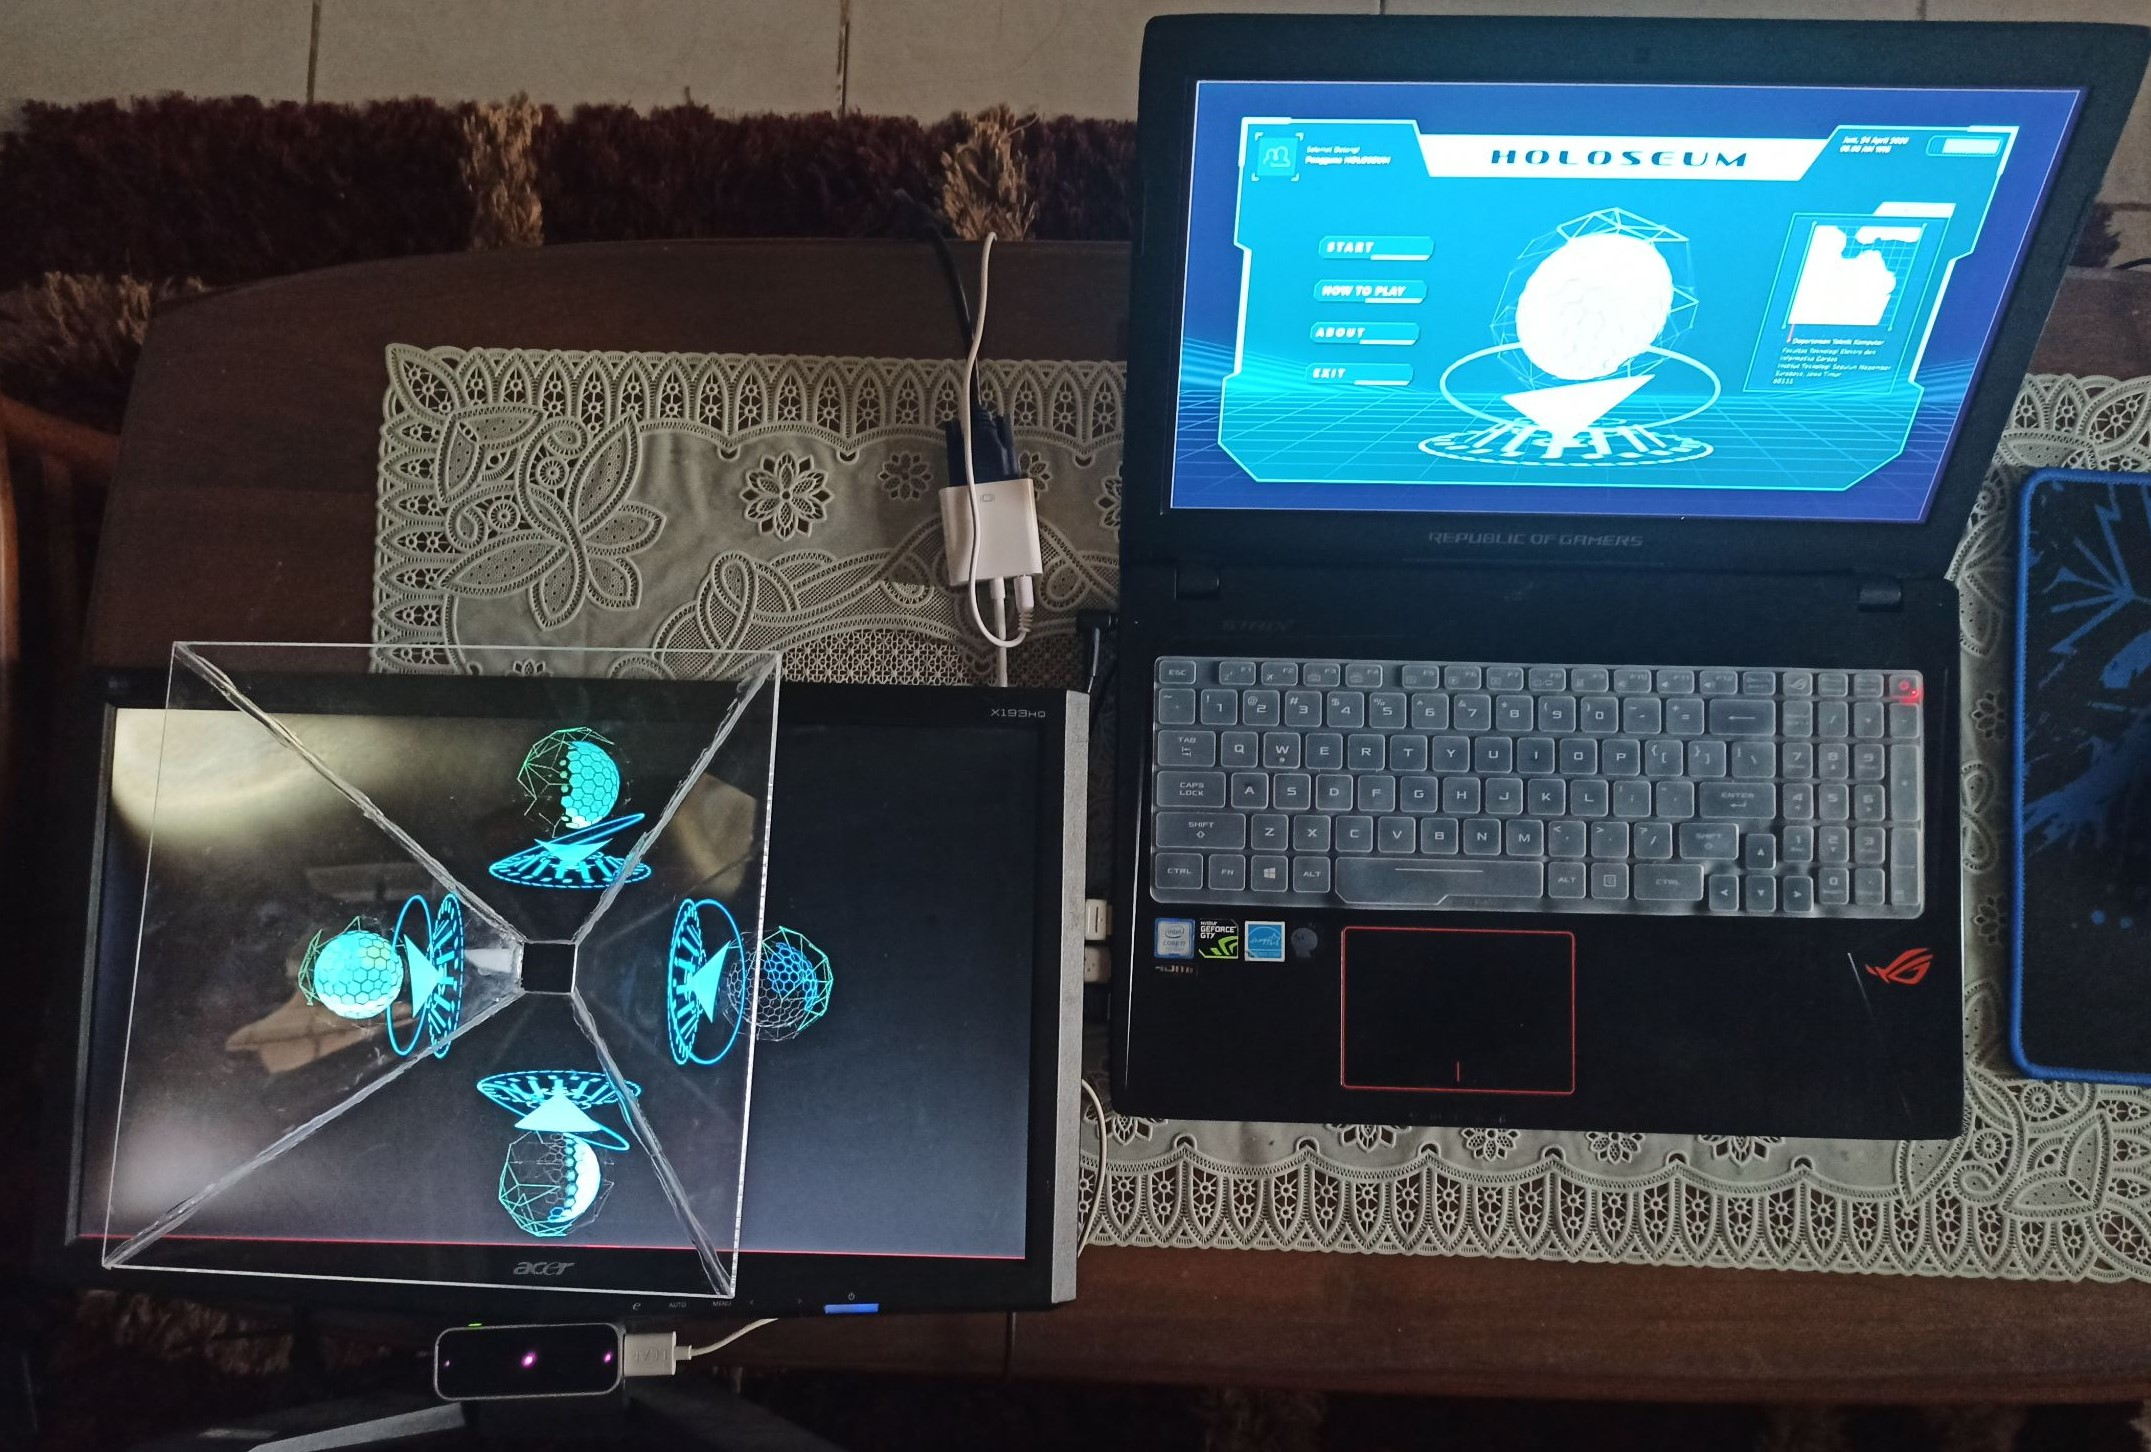
\includegraphics[width=0.8\textwidth]{img/bab3/foto_alat.jpg}
		\caption{Setting perangkat yang dibangun.}
		\label{fig:foto_alat}
	\end{figure}
\vspace{2ex}

\section{Implementasi Sistem Visualisasi} \label{section:visualisasi}
\vspace{1ex}
	Sistem visualisasi dibangun dengan memanfaatkan \textit{engine} Unity 2018.4.17f1. Dalam merealisasikan penelitian ini, digunakan dua monitor untuk menampilkan \textit{hologram video} dari objek hologram oleh \textit{display monitor} dan menampilkan menu aplikasi oleh \textit{information monitor}. Keduanya diprogram untuk dapat berjalan secara paralel.
\vspace{1.5ex}
	
	\subsection{Penyesuaian Objek Hologram}
	\vspace{1ex}
		Objek-objek berupa koleksi museum diperoleh dari asset 3D yang telah disediakan maupun hasil eksplorasi dari Sketchfab dengan referensi tertulis. Objek yang digunakan ditunjukkan pada gambar \ref{fig:objek3d}. Tabel \ref{fig:info_objek} menunjukkan informasi dari jumlah \textit{vertex} dan \textit{poly} objek 3D tersebut.
		\begin{figure} [H]
			\subfloat[\textit{Hand Axe}\cite{handaxe}.]{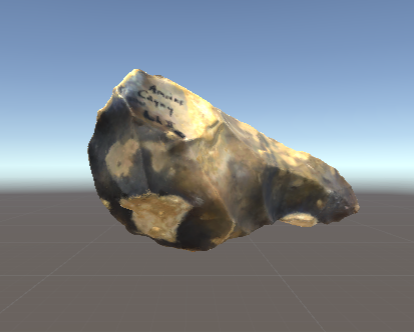
\includegraphics[width=0.32\textwidth]{img/obj/obj1_a.png}}
			\hspace{0.1em}
			\subfloat[\textit{Primeval Axe}\cite{primeval}.]{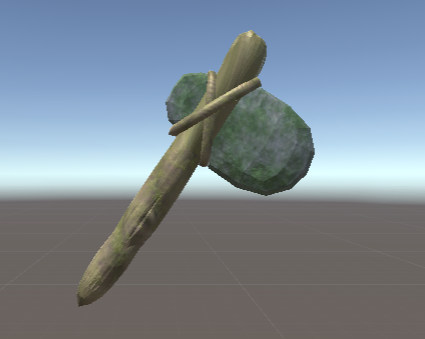
\includegraphics[width=0.32\textwidth]{img/obj/obj2_a.png}}
			\hspace{0.1em}
			\subfloat[\textit{Buddha Statue}\cite{buddha_lowpoly}.]{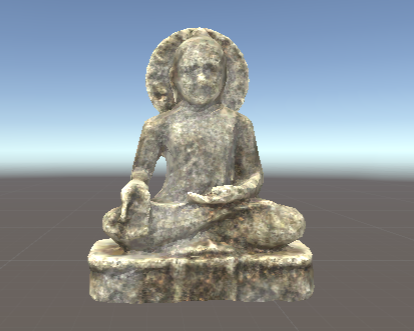
\includegraphics[width=0.32\textwidth]{img/obj/obj3_a.png}}
			\hspace{0.1em}
			\subfloat[\textit{Ganesha Statue}\cite{ganesha}.]{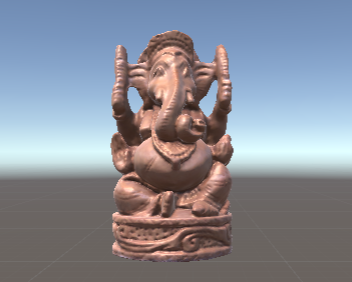
\includegraphics[width=0.32\textwidth]{img/obj/obj4_a.png}}
			\hspace{0.1em}
			\subfloat[\textit{Brass Lamp}\cite{brasslamp}.]{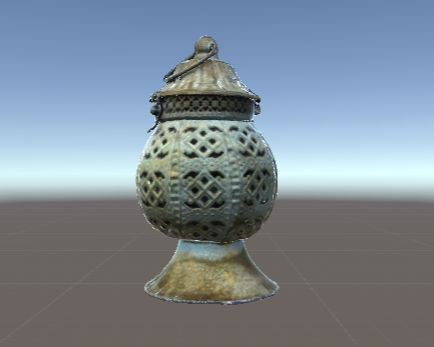
\includegraphics[width=0.32\textwidth]{img/obj/obj5_a.png}}
			\hspace{0.1em}
			\subfloat[\textit{Ceramic Pot}\cite{ceramicpot}.]{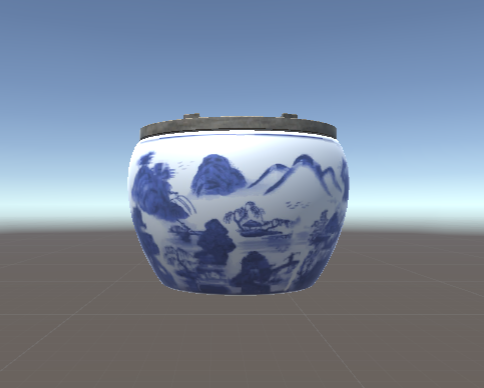
\includegraphics[width=0.32\textwidth]{img/obj/obj6_a.png}}
			\hspace{0.1em}
			\subfloat[\textit{Typewriter}\cite{typewriter}.]{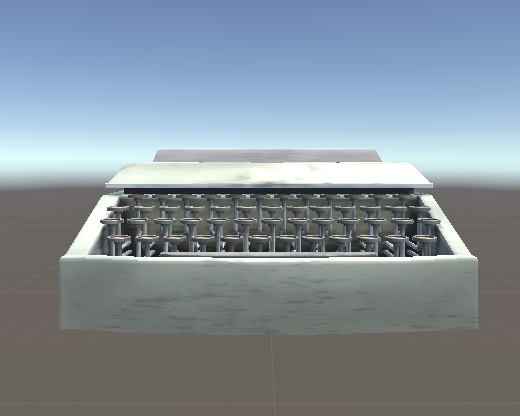
\includegraphics[width=0.32\textwidth]{img/obj/obj7_aa.png}}
			\hspace{0.1em}
			\subfloat[\textit{Gramophone}.]{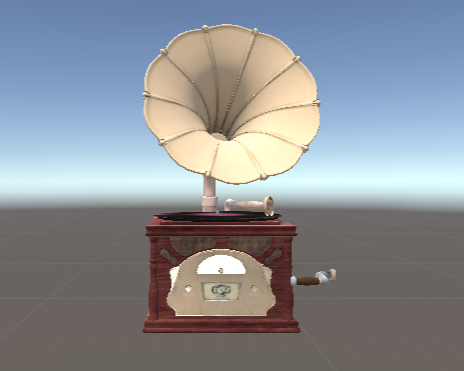
\includegraphics[width=0.32\textwidth]{img/obj/obj8_a.png}}
			\caption{Objek 3D yang digunakan pada penelitian.}
			\label{fig:objek3d}
		\end{figure}
		\vspace{-2ex}
	
		\begin{table}[H]
			\caption{Informasi jumlah \textit{poly} dan \textit{vertex} setiap objek 3D.}
			\label{fig:info_objek}
			\begin{tabular}{|c|l|L{2.5cm}|c|c|}
				\hline
				\textbf{No} & \multicolumn{1}{c|}{\textbf{Nama Objek}} & \multicolumn{1}{c|}{\textbf{Zona Peradaban}} & \textbf{\textit{Poly}} & \textbf{\textit{Vertex}} \\ \hline
				1.& \textit{Hand Axe}      & Purbakala            & 60000 & 30002  \\ \hline
				2.& \textit{Primeval Axe}  & Purbakala            & 1585  & 1180   \\ \hline
				3.& \textit{Buddha Statue} & Klasik 				 & 3000  & 1512   \\ \hline
				4.& \textit{Ganesha Statue}& Klasik 				 & 29124 & 14558  \\ \hline
				5.& \textit{Brass Lamp}    & Kolonial             & 27300 & 13640  \\ \hline
				6.& \textit{Ceramic Pot}   & Kolonial             & 1510  & 1522   \\ \hline
				7.& \textit{Typewriter}    & IPTEK                & 19218 & 18387   \\ \hline
				8.& \textit{Gramophone}    & IPTEK                & 17837 & 18682  \\ \hline
			\end{tabular}
		\end{table}
	
		Objek 3D yang diperoleh tidak dapat langsung direkonstruksi menjadi \textit{hologram video}, melainkan harus melalui proses penyesuaian terlebih dahulu. Pada dasarnya, penyesuaian ini terjadi melalui 2 proses menggunakan \textit{engine} yang berbeda. Untuk memodifikasi detail objek berdasarkan elemen penyusunnya, maka memerlukan aplikasi \textit{3D modelling} berupa Autodesk 3ds Max 2017. Contohnya untuk menambah atau mengurangi suatu elemen dalam objek tersebut seperti pada gambar \ref{fig:3dsmax}. Kemudian memindahkan titik poros objek pada posisi 0,0,0 yang ditunjukkan pada gambar \ref{fig:3dsmaxb} dengan tujuan agar objek hologram yang diinteraksikan seimbang tanpa terpotong \textit{workspace} yang dijelaskan lebih lengkap melalui \nameref{section:porosobjek}.
		\vspace{-2ex}
		\begin{figure} [H]
			\subfloat[Objek sebelum modifikasi\cite{buddha_lowpoly}.]{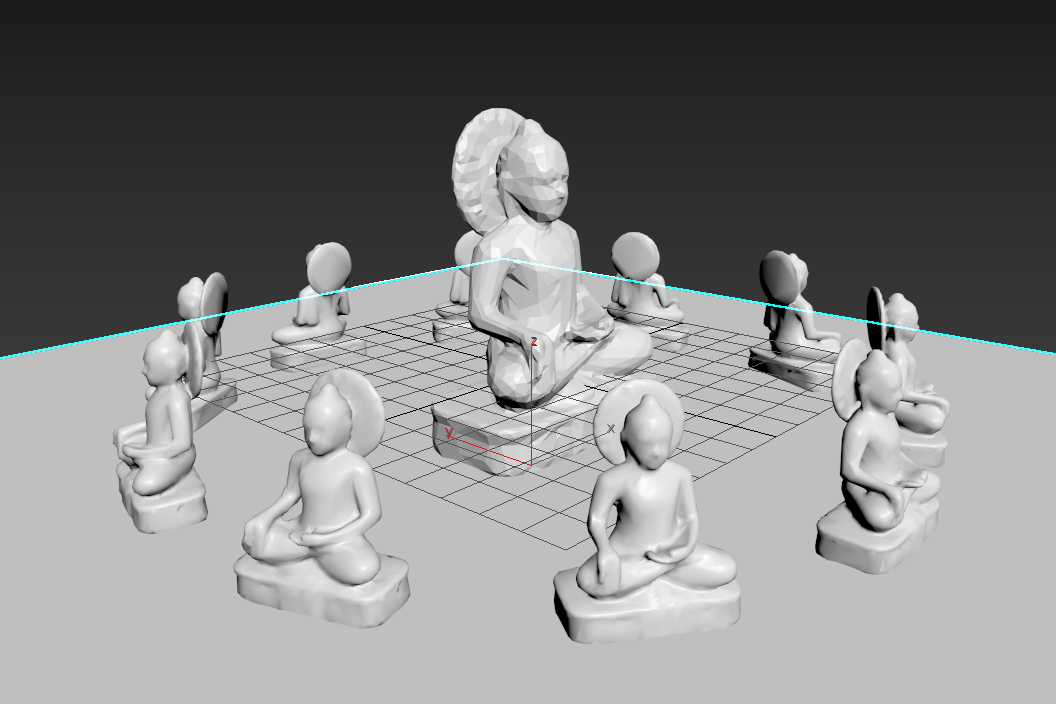
\includegraphics[width=0.47\textwidth]{img/bab3/buddha_banyak.png}}
			\hspace{0.1em}
			\subfloat[Objek setelah modifikasi.\label{fig:3dsmaxb}]{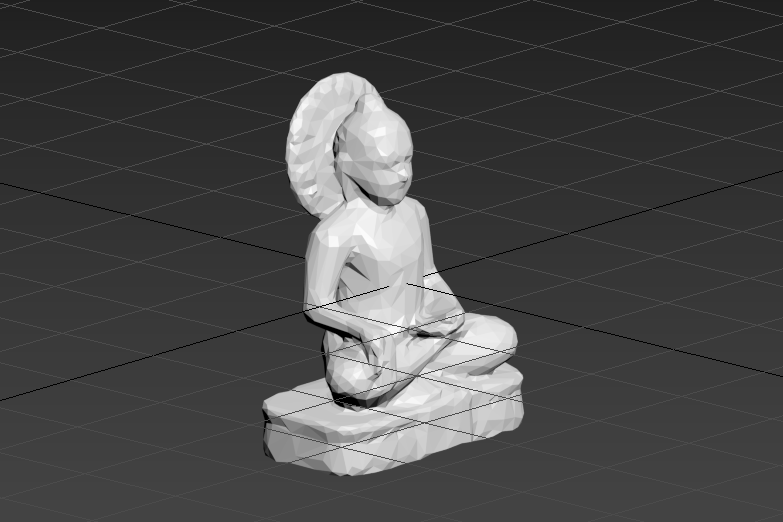
\includegraphics[width=0.47\textwidth]{img/bab3/buddha_1.png}}
			\caption{Penyesuaian objek pada Autodesk 3ds Max 2017.}
			\label{fig:3dsmax}
		\end{figure}
		\vspace{-2ex}
		
		Penyesuaian kedua menggunakan \textit{engine} Unity bertujuan mengatur objek dan membangun fitur pelengkap sebelum direkonstruksi menjadi \textit{hologram video}. Objek yang telah di-\textit{import} diatur posisi utama di tengah \textit{camera setting} dan disesuaikan ukurannya menggunakan \textit{scale}. Hubungan antara pengaturan posisi objek dan kamera akan dijelaskan pada bagian \nameref{section:rekonstruksi}. Setiap objek harus dipastikan telah melalui proses \nameref{section:standard} dan dilengkapi dengan komponen  \textit{collider} dan \textit{rigidbody}. \textit{Collider} berfungsi untuk memadatkan objek sehingga objek yang saling bertabrakan tidak akan saling menembus. Dalam penelitian ini, \textit{collider} dimanfaatkan untuk membuat \textit{workspace area} pergerakan objek 3D pada bagian \nameref{section:workspace}. Sedangkan \textit{rigidbody} berfungsi untuk memberikan efek gravitasi pada suatu objek, dimana jika ada gaya yang diberikan pada objek maka objek dapat 'merasakan' dan memberikan \textit{feedback}. Dalam penelitian ini, \textit{rigidbody} dimanfaatkan agar objek 3D dapat "melayang" pada \textit{workspace} yang dibangun. Pengaturan ini juga memungkinkan objek 3D dapat berputar (rotasi) dan bergerak dalam \textit{workspace area}. Pengaturan \textit{collider} dan \textit{rigidbody} ditunjukkan pada gambar \ref{fig:unity_colgid}. Penyesuaian pada tahap ini juga dimanfaatkan untuk membangun fitur respons berdasarkan gestur yang dimasukkan, seperti faktor pengali atau \textit{scale} untuk membangun fitur \textit{zoom} dan pengaturan posisi beserta rotasi dalam membangun fitur \textit{reset to default}. Selengkapnya dijelaskan pada bagian \nameref{section:implementasi_interaksi}. Sedangkan untuk memberikan efek hologram, maka yang harus diatur adalah material dan \textit{shader} yang membangun objek tersebut. Penyesuaian untuk memberikan efek hologram dilakukan hingga mencapai efek yang dihendaki. Selain itu, penyesuaian di Unity juga dapat dimanfaatkan untuk menciptakan animasi dengan memindah, memutar, atau mengatur ukuran komponennya.
		\begin{figure} [H]
			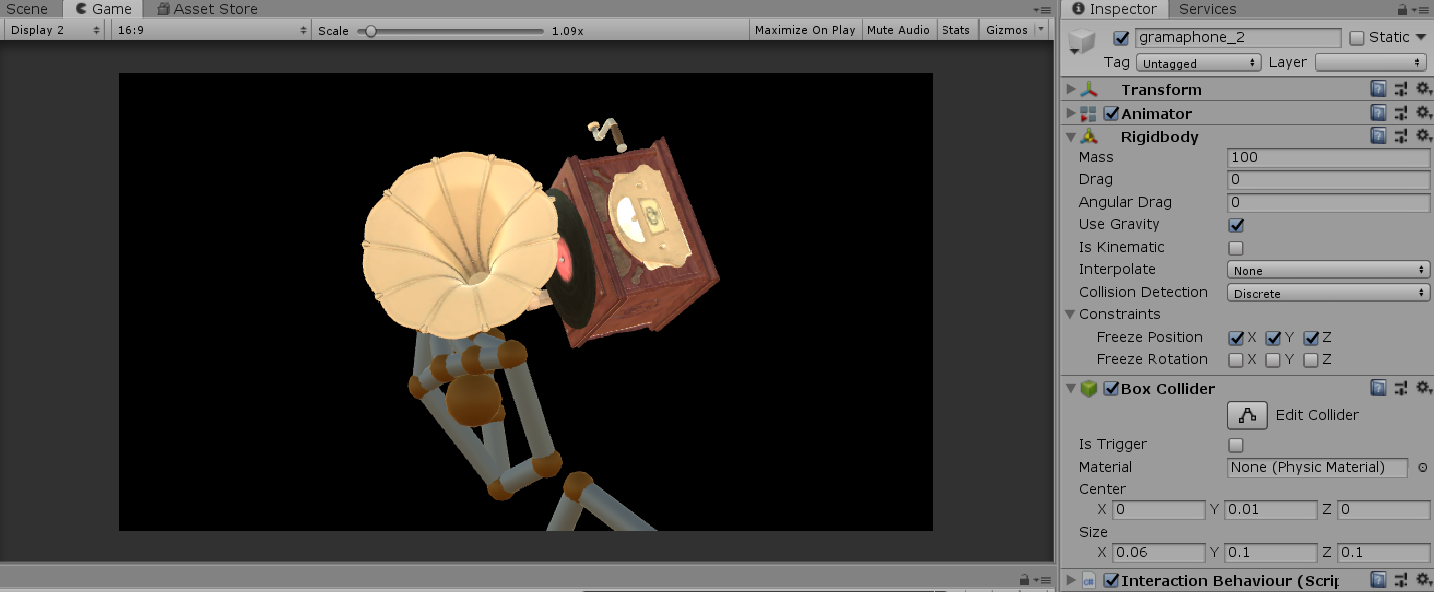
\includegraphics[width=0.9\textwidth]{img/bab3/unity_colgid.png}
			\caption{Penyesuaian melalui \textit{collider} dan \textit{rigidbody} pada Unity.}
			\label{fig:unity_colgid}
		\end{figure}
		\begin{comment}
		Sedangkan untuk memberikan efek hologram, maka yang harus diatur adalah material dan \textit{shader} yang membangun objek tersebut. Material pada Unity disediakan oleh \textit{shader Standard} dan \textit{shader Standard Specular Setup} (gambar \ref{fig:unity_material}). \textit{Specular Setup} langsung mengatur tingkat kecerahan dari specularnya langsung, sedangkan \textit{Metallic Setup} pada \textit{shader Standard} harus mengatur parameter lain dan efek specularnya muncul karena perubahan itu\cite{unity_spec}. Penyesuaian untuk memberikan efek hologram dilakukan hingga mencapai efek yang dihendaki.
		\begin{figure} [H]
			\subfloat[\textit{Shader Standard}.]{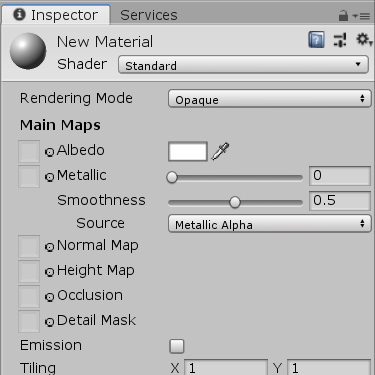
\includegraphics[width=0.47\textwidth]{img/bab3/standard.png}}
			\hspace{0.1em}
			\subfloat[\textit{Shader Standard Specular}.]{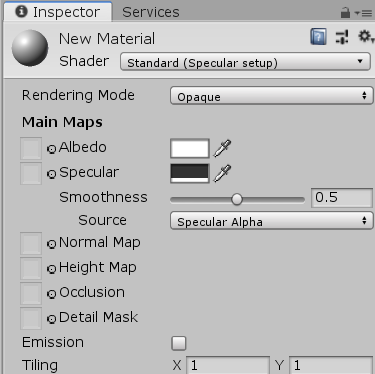
\includegraphics[width=0.47\textwidth]{img/bab3/standard_specular.png}}
			\caption{Perbedaan material \textit{shader} pada Unity.}
			\label{fig:unity_material}
		\end{figure}
		\end{comment}
				\vspace{1ex}
		
		\subsubsection{Penyesuaian Titik Poros Objek} \label{section:porosobjek}
		\vspace{0.5ex}
			\begin{figure} [!h]
				\subfloat[Titik poros asli objek pada Autodesk 3ds Max 2017.\label{fig:000bawah}]{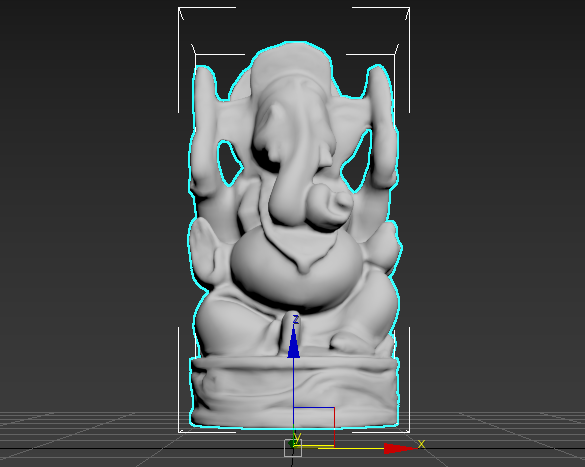
\includegraphics[width=0.47\textwidth]{img/bab3/000bawah.png}}
				\hspace{0.1em}
				\subfloat[Titik poros objek baru pada Autodesk 3ds Max 2017.\label{fig:000tengah}]{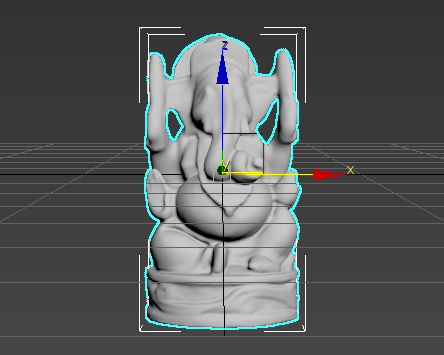
\includegraphics[width=0.47\textwidth]{img/bab3/000tengah.png}}
				\hspace{0.1em}
				\subfloat[Titik poros asli objek pada Unity.\label{fig:000bawah_unity}]{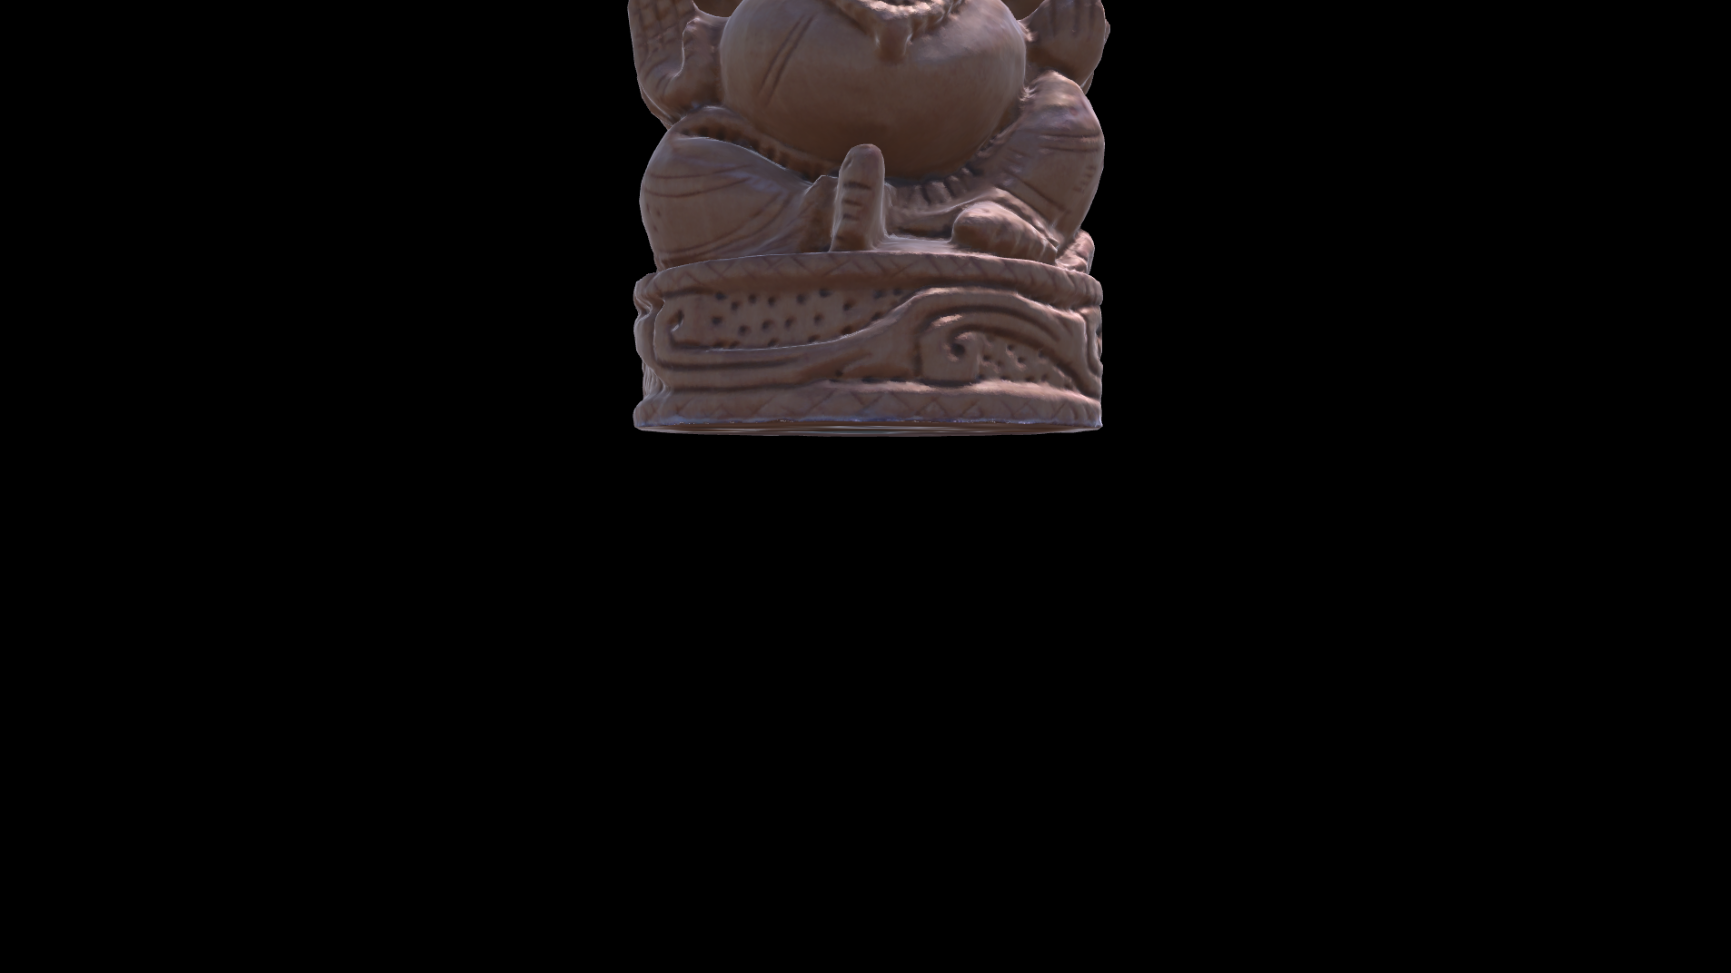
\includegraphics[width=0.47\textwidth]{img/bab3/000bawah_unity.png}}
				\hspace{0.1em}
				\subfloat[Titik poros objek baru pada Unity.\label{fig:000tengah_unity}]{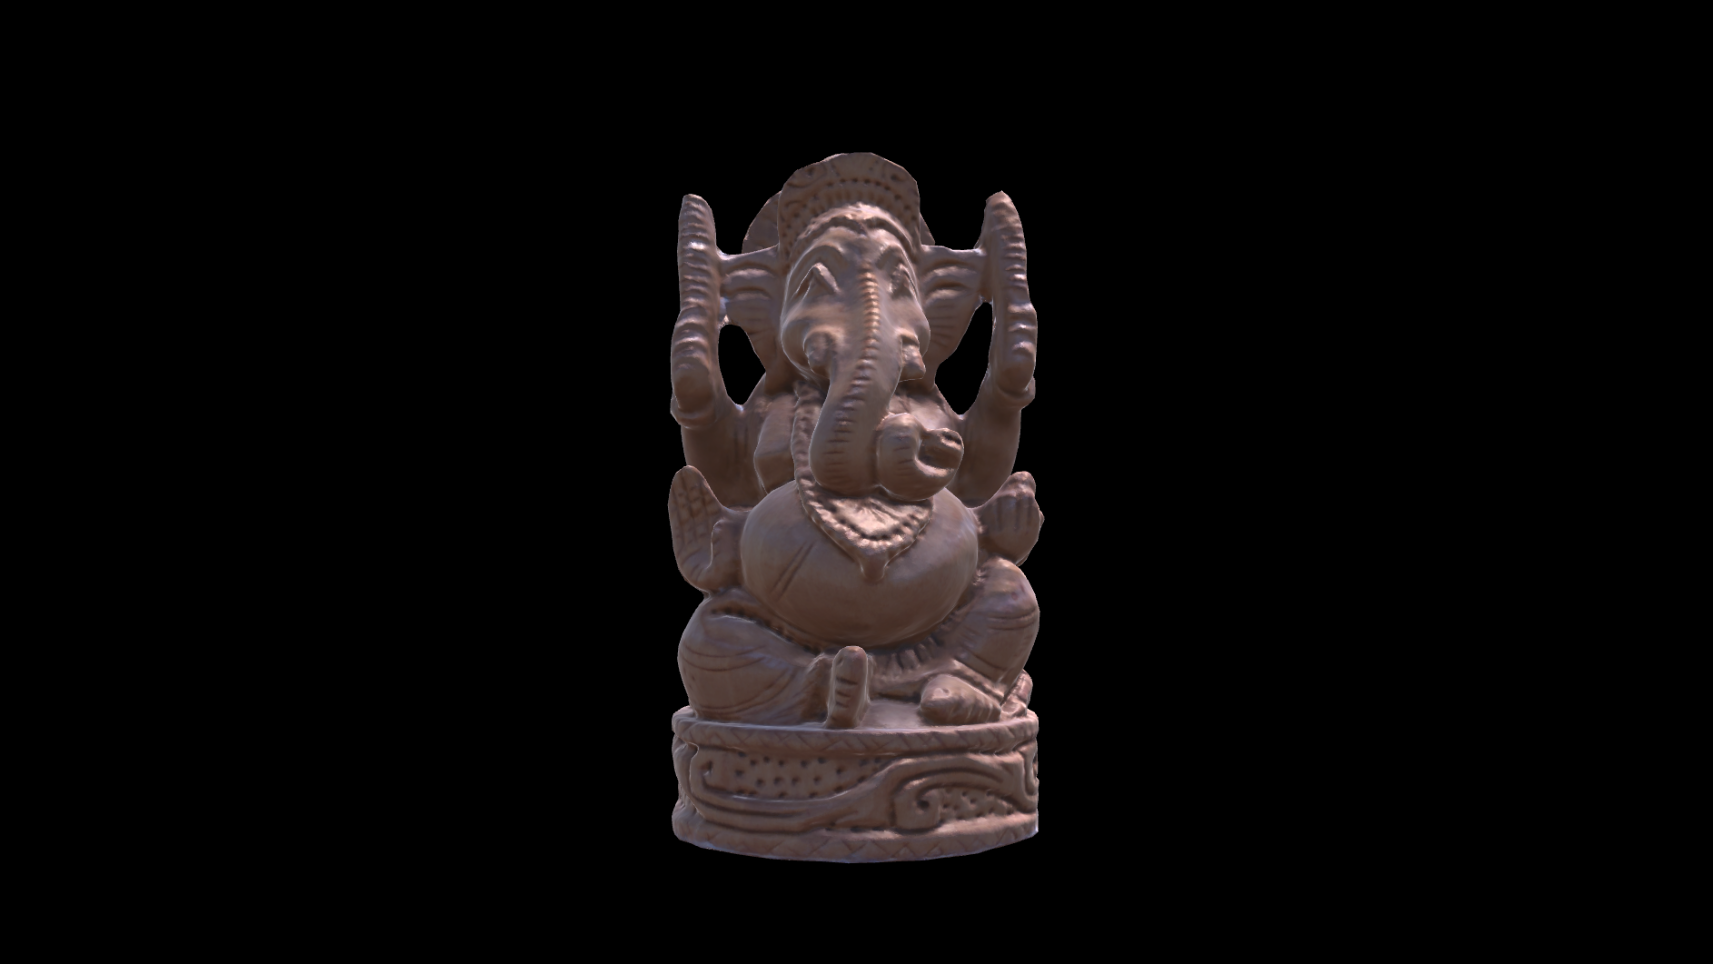
\includegraphics[width=0.47\textwidth]{img/bab3/000tengah_unity.png}}
				\hspace{0.1em}
				\subfloat[Objek dengan titik poros asli pada saat diputar.\label{fig:000bawah_unity2}]{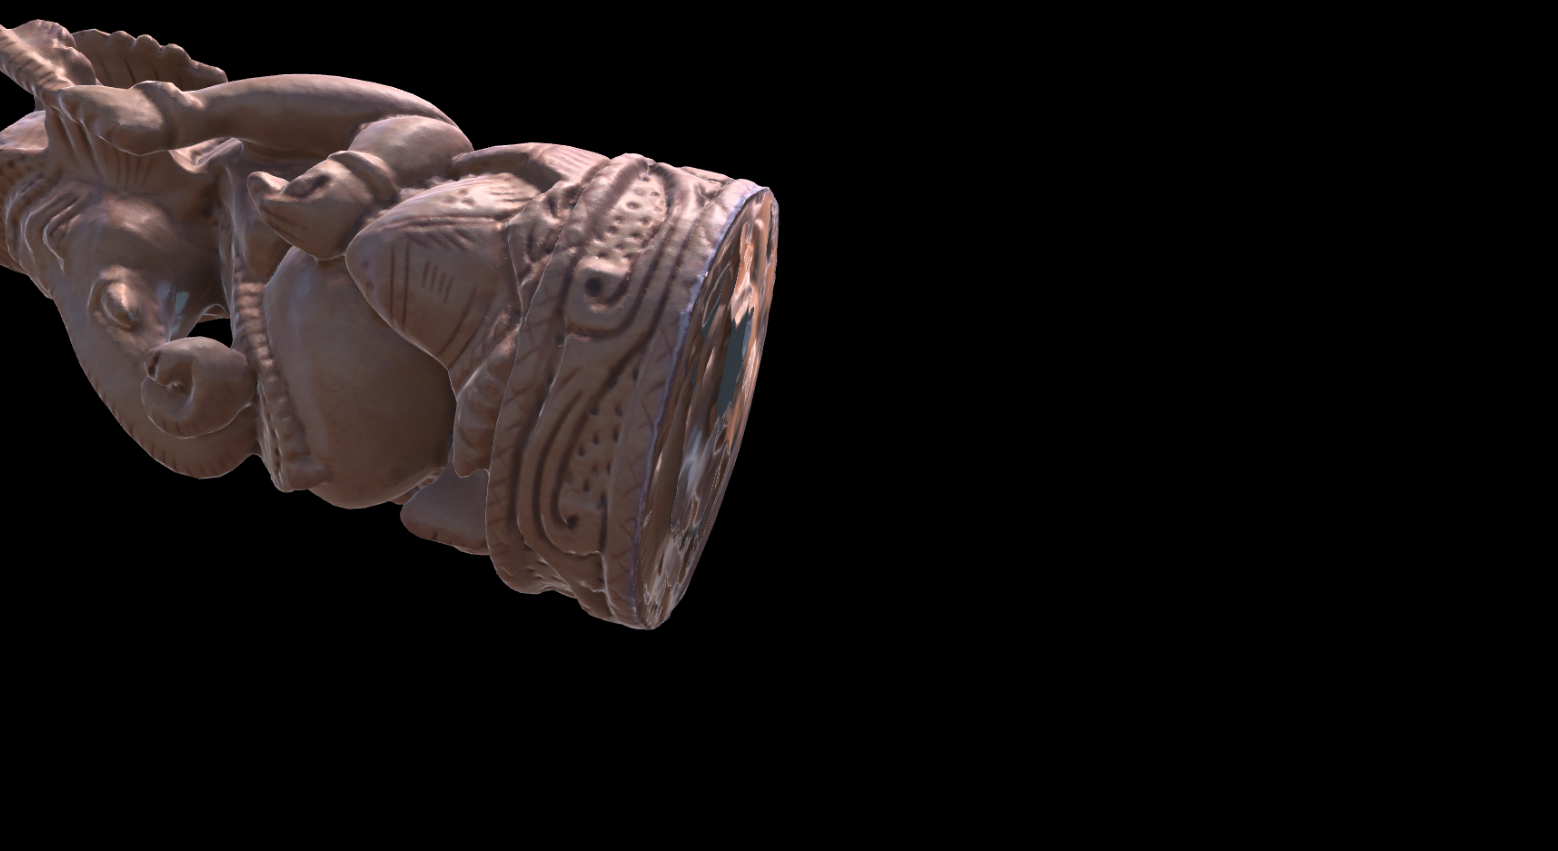
\includegraphics[width=0.47\textwidth]{img/bab3/000bawah_unity2.png}}
				\hspace{0.1em}
				\subfloat[Objek dengan titik poros baru pada saat diputar.\label{fig:000tengah_unity2}]{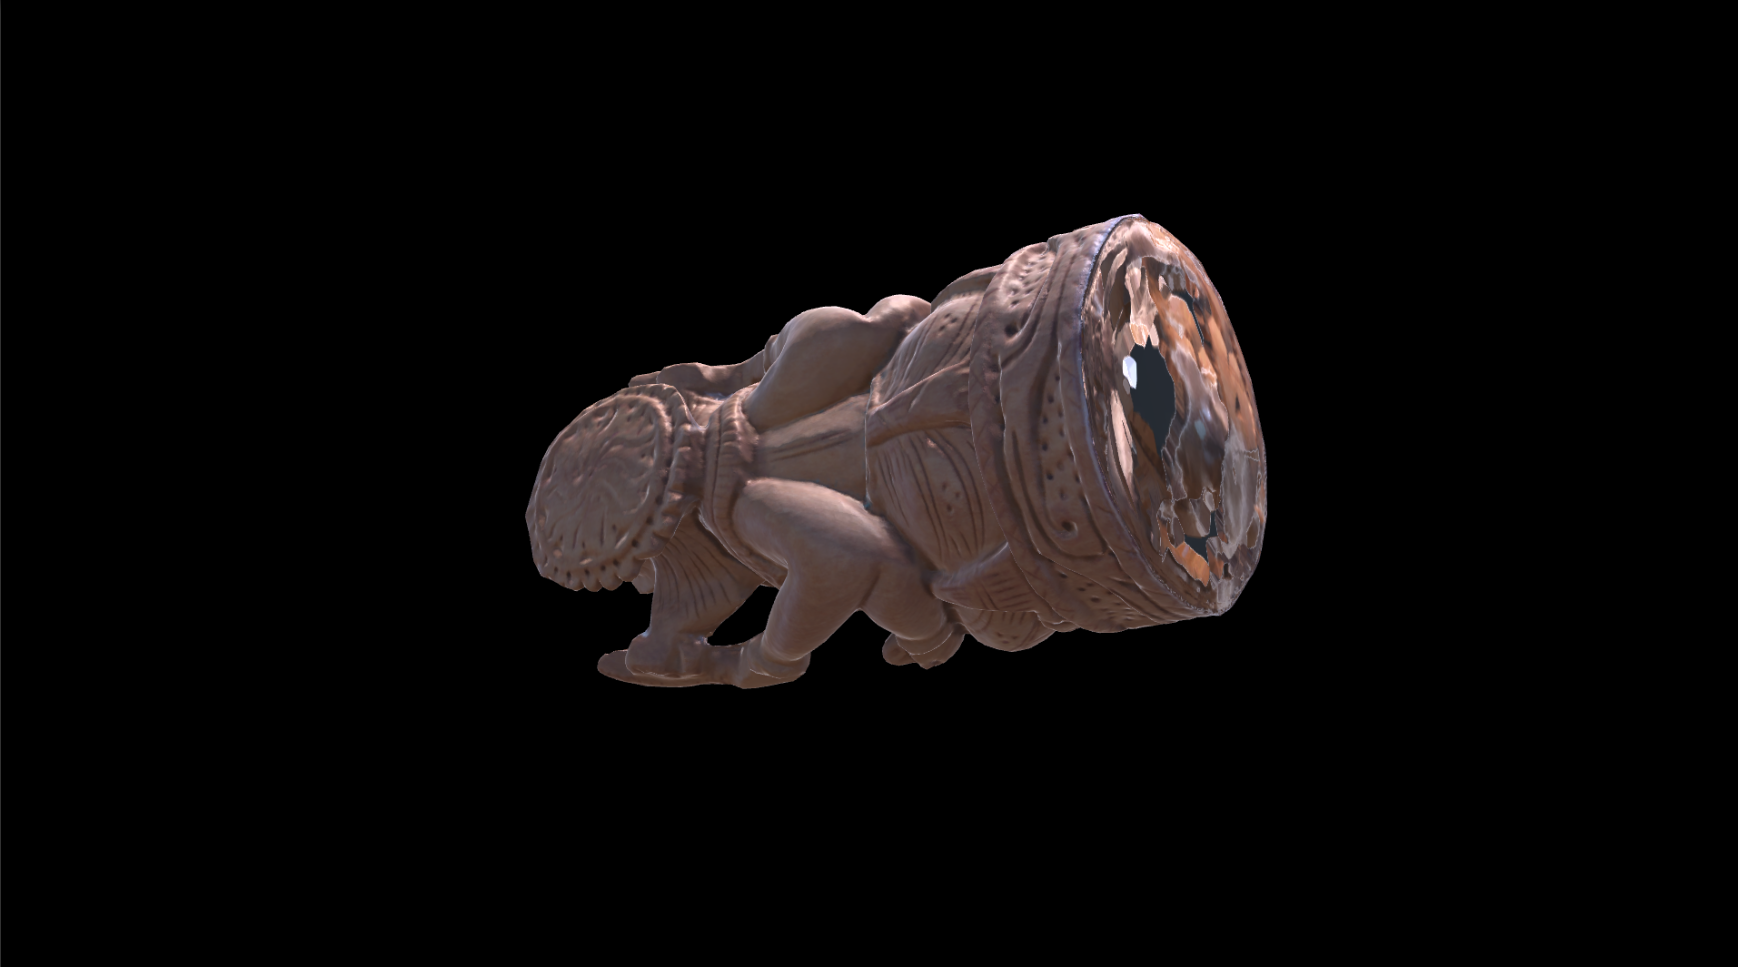
\includegraphics[width=0.47\textwidth]{img/bab3/000tengah_unity2.png}}
				\caption{Efek pemindahan titik poros objek.}
				\label{fig:pindahporos}
			\end{figure}
			
			%kenapa harus dipindah
			Setiap objek memiliki titik poros yang berbeda dikarenakan titik poros ditentukan oleh 3D \textit{artist} yang membuat objek 3D tersebut yang bebas diletakkan dimana saja. Pemindahan ini bertujuan untuk menyeragamkan titik poros dari seluruh objek 3D yang digunakan. Perbedaan titik poros tiap objek yang digunakan mempengaruhi perspektif antara pengguna dan objek khususnya pada proses rotasi objek. Rotasi memerlukan titik poros perputaran sehingga untuk membuat objek dapat berputar dengan seimbang pada workspace yang ditentukan, maka titik poros objek harus diletakkan tepat pada tengah objek tersebut. Pada penelitian ini, rotasi objek 3d dilakukan berdasarkan pergerakan tangan (lihat \nameref{section:eksplorasi}) sehingga dibutuhkan orientasi yang sama antara objek dengan tangan pengguna. Efek dari pemindahan titik poros objek ditunjukkan pada gambar \ref{fig:pindahporos}. Pada gambar \ref{fig:000bawah}, objek asli memiliki titik poros pada tengah di bawah objek sehingga jika diputar maka menghasilkan gambar \ref{fig:000bawah_unity2} dimana ada bagian yang terpotong workspace saat dirotasikan. Sedangkan pada gambar \ref{fig:000tengah} saat titik poros objek dipindahkan  tepat pada tengah objek, sehingga saat diputar maka menghasilkan gambar \ref{fig:000tengah_unity2} dimana perputarannya lebih seimbang tanpa memotong objek yang ditampilkan pada pengguna.
			
			%kenapa dipindahnya ke 0,0,0
			Titik poros objek dipindah ke 0,0,0 agar saat di import ke Unity, penempatan objek sesuai dengan inisialisasi \textit{transform} pada Unity. Saat titik poros tidak tepat pada tengah objek di titik 0,0,0 sesuai gambar \ref{fig:000bawah}, maka selisih antara titik poros asli dengan titik tengah seharusnya akan memengaruhi \textit{transform} pada Unity yang ditunjukkan pada gambar \ref{fig:000bawah_unity}. Sedangkan jika titik poros objek tepat di tengah objek pada posisi 0,0,0 sesuai gambar \ref{fig:000tengah}, maka tidak ada selisih yang menyebabkan posisi objek dapat diatur langsung melalui \textit{transform} Unity sehingga objek tetap berada di tengah dan tetap seimbang seperti gambar  \ref{fig:000tengah_unity}. Objek diletakkan tepat di titik 0,0,0 pada Unity yang menjadi titik fokus pandangan pengguna.
		\vspace{0.75ex}
		
		\subsubsection{Pengaturan Nilai Standard Objek} \label{section:standard}
		\vspace{0.5ex}
			Setiap objek memiliki standard yang berbeda-beda dikarenakan nilai perhitungan yang bebeda pula. Pada penelitian ini, standard objek yang harus didefinisikan terlebih dahulu di antaranya nilai posisi awal, nilai rotasi awal, nilai minimum dan maksimum perbesaran yang ditunjukkan pada gambar \ref{fig:eachobject}. Khusus untuk nilai minimum dan maksimum \textit{workspace area} dijelaskan pada \nameref{section:workspace}. Pendefinisian ini bermanfaat untuk mengembalikan objek pada keadaan awal pada \textit{reset to default} dan mendapatkan nilai perhitungan ukuran objek pada \textit{zoom object}. Hal ini dikarenakan pada setiap pergantian frame, nilai posisi, rotasi, dan ukuran objek selalu diperbarui. Untuk posisi dan rotasi objek, objek berpindah dan berputar saat eksplorasi atau \textit{reset to default} dilakukan selama berada dalam \textit{workspace area} yang didefinisikan seperti pada flowchart \ref{fig:standard_pr}. Sedangkan ukuran objek, objek akan berganti ukuran saat \textit{zoom object} atau \textit{reset to default} berlangsung sesuai flowchart \ref{fig:standard_s}. 
			\begin{figure}[H]
				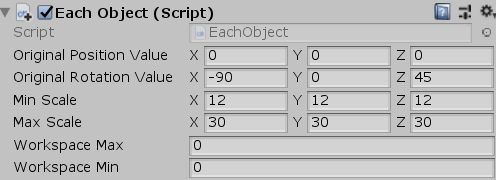
\includegraphics[width=0.75\textwidth]{img/bab3/eachobject.png}
				\caption{Pengaturan nilai standard objek pada Unity.}
				\label{fig:eachobject}
			\end{figure}
			\vspace{-2ex}
			\begin{figure} [H]
				\subfloat[Perubahan posisi dan rotasi.\label{fig:standard_pr}]{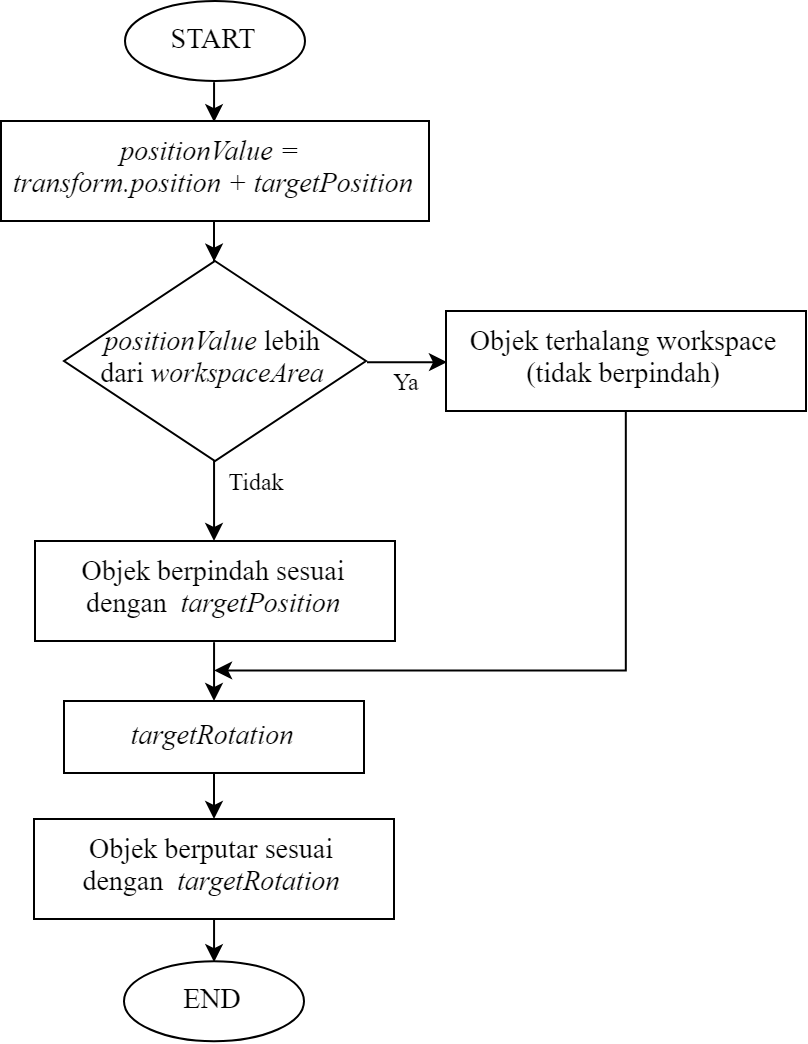
\includegraphics[width=0.47\textwidth]{img/bab3/standard_pr.png}}
				\hspace{0.1em}
				\subfloat[Perubahan ukuran objek.\label{fig:standard_s}]{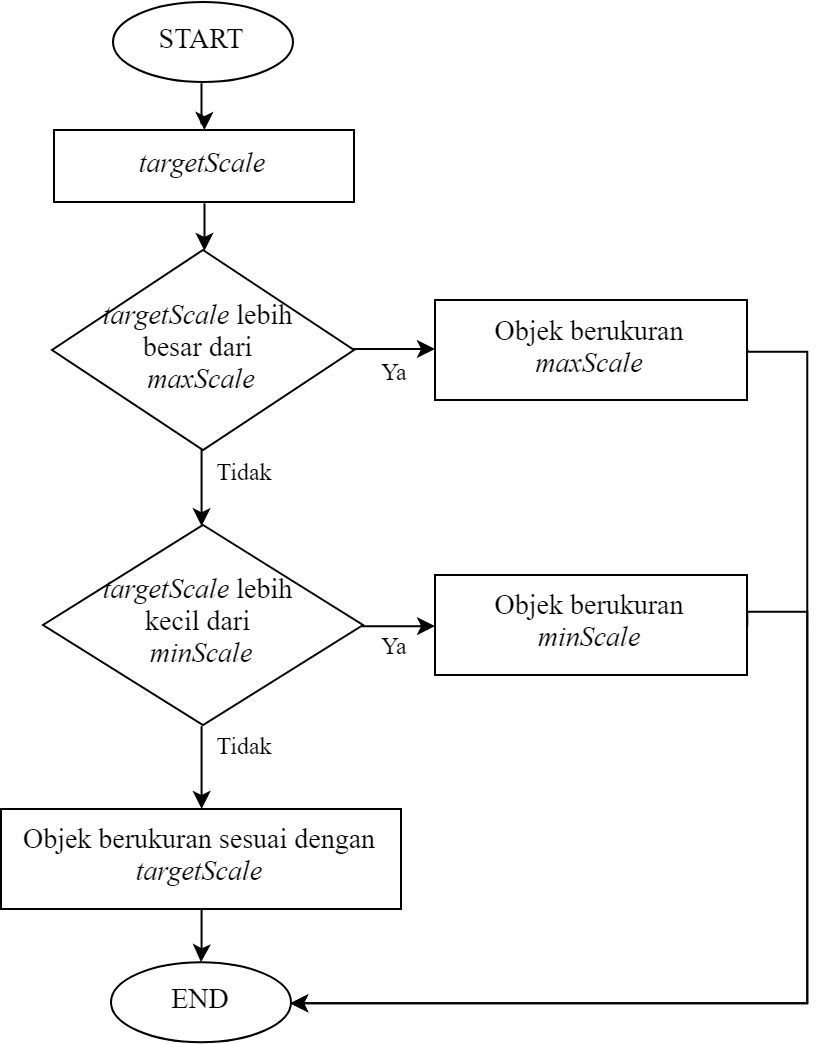
\includegraphics[width=0.47\textwidth]{img/bab3/standard_s.png}}
				\caption{Mekanisme pembaruan nilai rotasi, posisi, dan ukuran pada setiap objek.}
				\label{fig:standard_flowchart}
			\end{figure}
		\vspace{0.75ex}
		
		\subsubsection{Penyesuaian \textit{Workspace Area} Objek} \label{section:workspace}
		\vspace{0.5ex}
			\textit{Workspace area} objek didefinisikan sebagai daerah yang akan terlihat oleh pengguna melalui \textit{display monitor} yang membatasi pergerakan objek pada eksplorasi objek. Pada penelitian ini, pembangunan \textit{workspace area} memanfaatkan \textit{bounding box} yang dimiliki oleh \textit{collider} setiap objek. \textit{Boundary box} yang dimaksud merupakan kotak pembatas yang didapatkan dari pengolahan titik tengah, ukuran, dan nilai minimal maupun maksimal dari \textit{bounds collider}. %tersebut sesuai pada kode \ref{lst:bounds_workspace}. 
			Besarnya \textit{workspace objek} bergantung dari ukuran objek yang sedang diaktifkan sehingga setiap objek membutuhkan nilai minimum dan maksimum skala (\textit{minScale} dan \textit{maxScale}) yang didefinisikan pada \nameref{section:standard}. Sehingga titik maksimal pergerakan objek berada pada titik terjauh \textit{bounds} sesuai pada persamaan \ref{eqn:bounds_workspace}.
			\begin{equation}
			workspaceValue = m\_CenterValue + \frac{1}{2} m\_SizeValue
			\label{eqn:bounds_workspace}
			\end{equation}
			
			\begin{comment}
			\begin{lstlisting}[caption=Penentuan \textit{workspace area} dalam \Csh{} \textit{code}, label=lst:bounds_workspace]
public void GetWorkspace()
{
   m_Collider = GetComponent<Collider>();
   m_Center = m_Collider.bounds.center;
   m_Size = m_Collider.bounds.size;
   m_Min = m_Collider.bounds.min;
   m_Max = m_Collider.bounds.max;
   workspaceMax = Mathf.Max(m_Max.x,m_Max.y,m_Max.z);
   workspaceMin = -maxPosition;
}
			\end{lstlisting}		
			\end{comment}
	\vspace{1.5ex}
		
	\subsection{Rekonstruksi \textit{Hologram Video}} \label{section:rekonstruksi}
	\vspace{1ex}
		Objek 3D yang telah disesuaikan selanjutnya direkonstruksi menjadi \textit{hologram video} agar dapat diproyeksikan dengan \textit{pyramid hologram}. Hal ini bertujuan untuk menyesuaikan tampilan pada monitor dengan mengatur penempatan objek 3D tepat di setiap sisi \textit{pyramid hologram}. \textit{Pyramid hologram} yang digunakan berjenis 4 sisi, sehingga membutuhkan sebuah \textit{game view} (pada Unity) yang seolah-olah menampilkan 4 buah objek yang diatur seperti tanda tambah (+). Setiap sisi \textit{hologram video} menampilkan \textit{viewing angle} sebesar 90° dari objek 3D tersebut sehingga jika dapat melihat keseluruhan objek dari sisi piramida yang berbeda.
		\begin{figure} [H]
			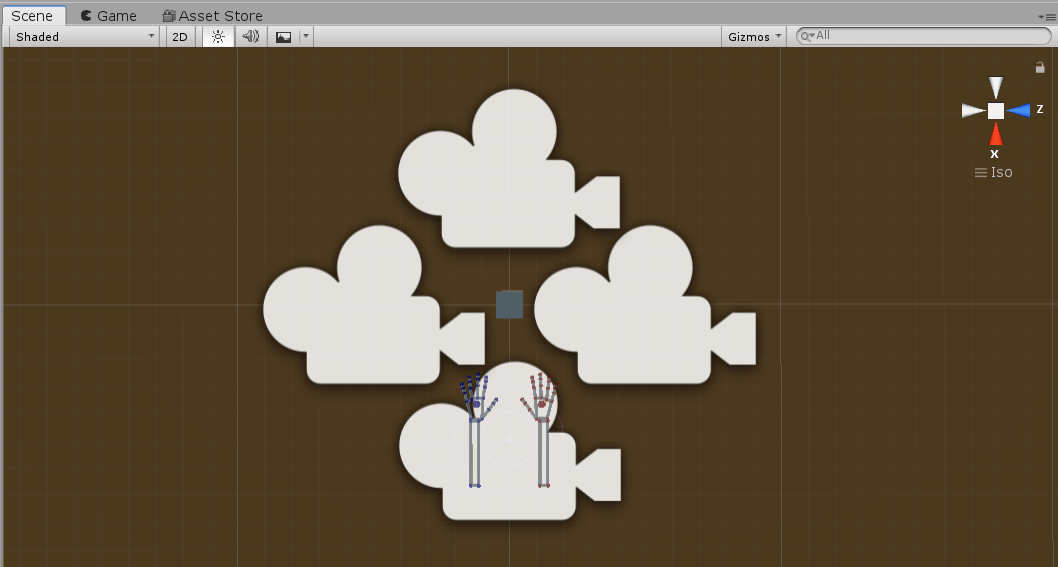
\includegraphics[width=0.9\textwidth]{img/bab3/unity_4cam.png}
			\caption{Posisi \textit{main camera} terhadap objek di Unity.}
			\label{fig:unity_4cam}
		\end{figure}
		\vspace{-2ex}
		
		Untuk menampilkan 4 posisi objek pada 1 \textit{game view} seperti gambar \ref{fig:desain_dm}, pengaturan yang diterapkan pada penelitian ini berupa sebuah objek 3D yang dikelilingi oleh 4 \textit{main camera} yang berbeda. Salah satu \textit{main camera} yang digunakan merupakan kamera yang disediakan oleh Leap Motion. Jarak antara setiap kamera terhadap objek 3D yang ditampilkan sama besar. Agar tidak perlu mengatur posisi kamera pada objek yang berbeda, maka faktor skala digunakan untuk menyesuaikan ukuran dari objek 3D. Posisi kamera terhadap objek ini ditunjukkan pada gambar \ref{fig:unity_4cam}.
		
		Untuk mendapatkan tampilan dari 4 \textit{main camera} yang membentuk tanda tambah (+) pada 1 \textit{game view} seperti gambar \ref{fig:unity_12cam}, maka membutuhkan 7 \textit{hidden camera} untuk menampilkan \textit{background} hitam. Posisi dari 7 \textit{hidden camera} diatur sejauh mungkin dari \textit{main camera}. Pengaturan yang terlibat pada bagian ini adalah \textit{viewport} dari setiap kamera yang digunakan. Pada Unity, \textit{viewport} adalah \textit{on screen area} yang memiliki rentang antara 0 dan 1 dengan posisi (0,0) berada di pojok kiri bawah dan (1,1) berada di pojok kanan atas. Sehingga diperlukan pengaturan ukuran dan posisi untuk setiap kamera yang digunakan. Ukuran (\textit{weight} (W) dan \textit{height} (H)) setiap kamera adalah 0.2 dan 0.333. Pengaturan posisi kamera ditunjukkan pada gambar \ref{fig:unity_12cam}. 
		\begin{figure} [H]
			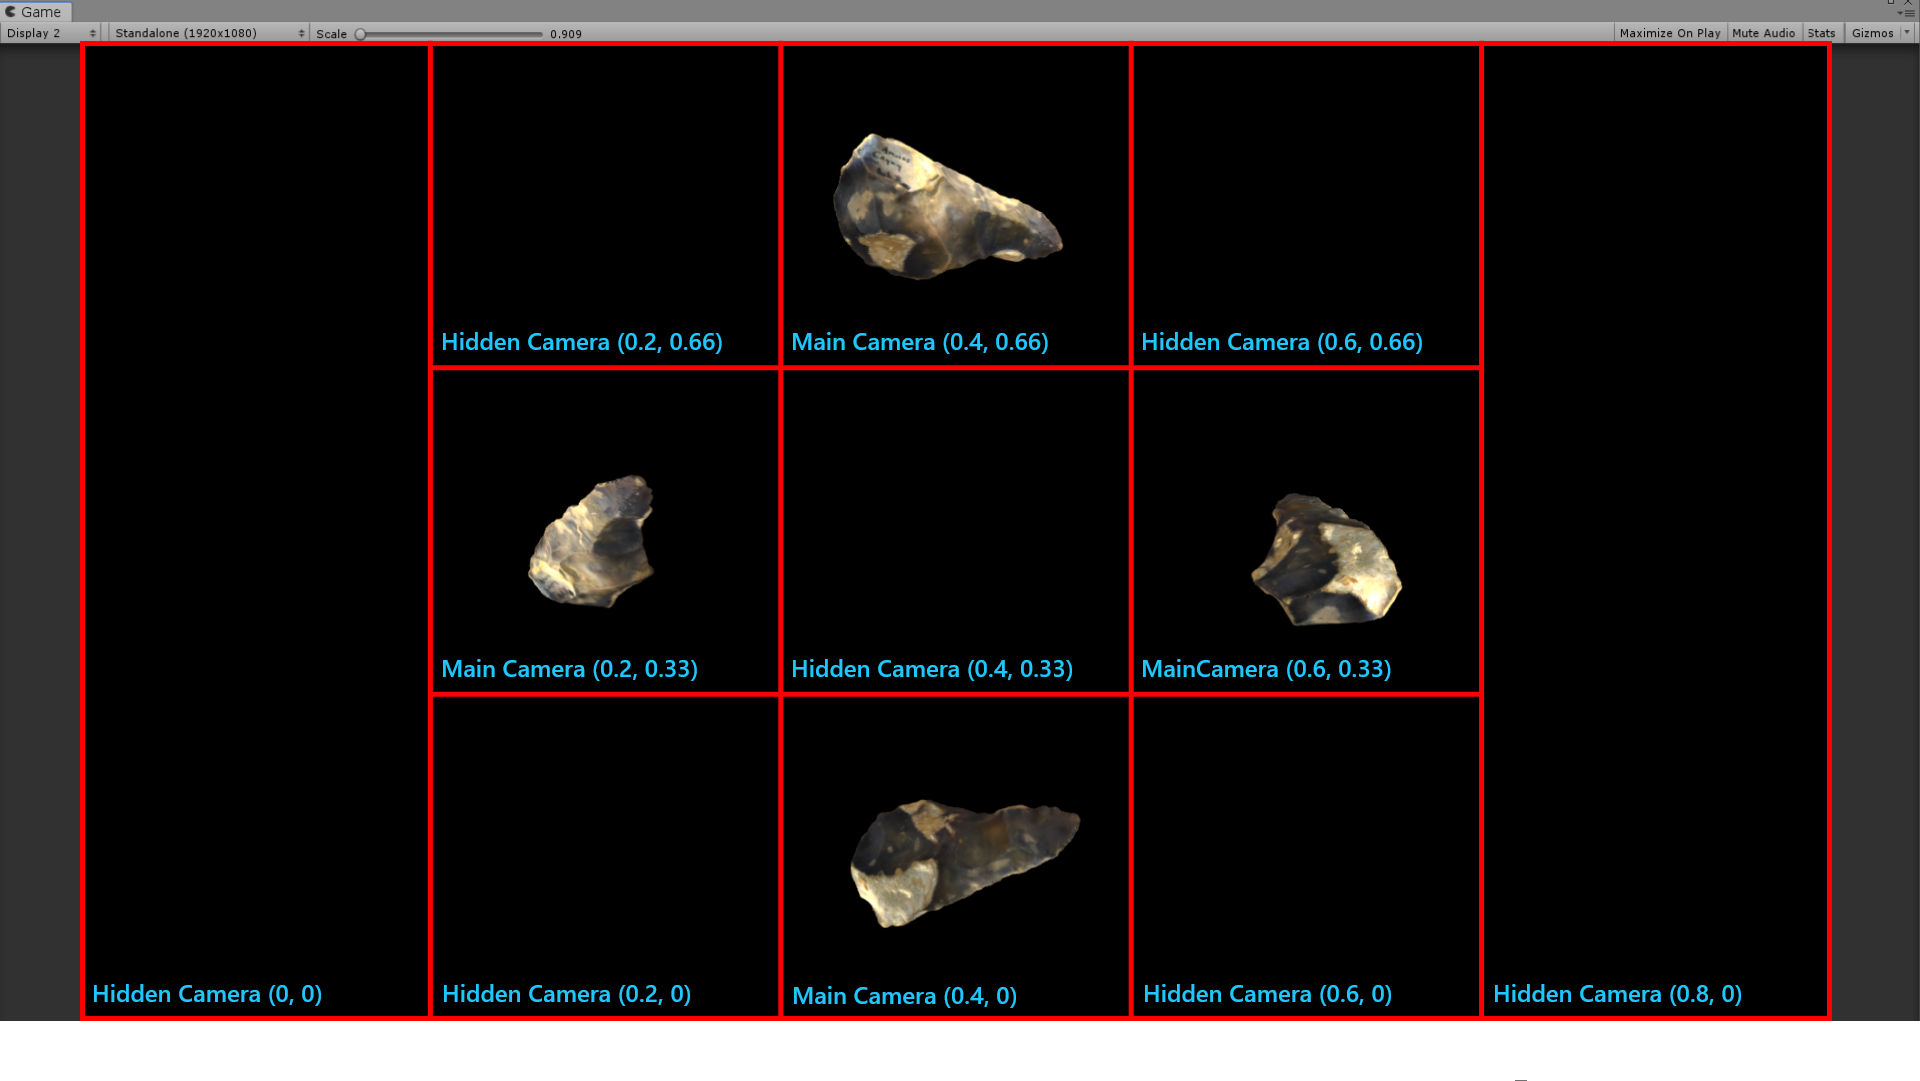
\includegraphics[width=\textwidth]{img/bab3/unity_12cam.png}
			\caption{Pengaturan \textit{viewport} untuk \textit{hologram video}.}
			\label{fig:unity_12cam}
		\end{figure}
	\vspace{1.5ex}
	
	\subsection{Realisasi \textit{User Interface} Aplikasi}
	\vspace{1ex}
		Asset berupa tombol dan ikon pada tabel \ref{tab:asset_aplikasi} beserta supergrafis yang digunakan dalam membuat tampilan aplikasi dibuat menggunakan \textit{engine} Adobe XD kemudian disesuaikan dengan konfigurasi pada Unity.
		\vspace{-2ex}
		\begin{table}[h]
		\caption{Asset tombol dan ikon pada tampilan aplikasi.}
		\label{tab:asset_aplikasi}
			\begin{tabular}{|C{3 cm}|C{3 cm}|C{3 cm}|}
				\hline 
				\multicolumn{3}{|c|}{
\includegraphics[width=0.3\linewidth]{img/bab3/button/start_sblm.png}} \\
				\multicolumn{3}{|c|}{Tombol  untuk memulai permainan menuju \textit{Main Scene}.} \\ \hline
				
\includegraphics[width=\linewidth]{img/bab3/button/htp_sblm.png}&
				
\includegraphics[width=\linewidth]{img/bab3/button/about_sblm.png}&
				\includegraphics[width=\linewidth]{img/bab3/button/exit_sblm.png} \\ 
				Tombol untuk memulai panduan permainan.&
				Tombol untuk  informasi produk dan \textit{developer}.& 
				Tombol untuk keluar dari aplikasi.\\ \hline
				\includegraphics[width=0.7\linewidth]{img/bab3/button/back_sblm.png}&
				\includegraphics[width=0.7\linewidth]{img/bab3/button/cancel_sblm.png}&
				\includegraphics[width=0.7\linewidth]{img/bab3/button/ok_sblm.png} \\ 
				Tombol untuk kembali ke tampilan sebelumnya.\label{fig:tb_back}&
				Tombol untuk membatalkan perintah yang ditampilkan.\label{fig:tb_cancel}& 
				Tombol untuk menyetujui perintah yang ditampilkan.\label{fig:tb_ok}\\ \hline
				\includegraphics[width=0.2\linewidth]{img/bab3/button/kiri_sblm.png}&
				\includegraphics[width=0.2\linewidth]{img/bab3/button/kanan_sblm.png}&
				\includegraphics[width=0.2\linewidth]{img/bab3/button/mm_sblm.png} \\ 
				Tombol untuk menampilkan opsi sebelumnya pada suatu menu.\label{fig:ikon_prev}&
				Tombol untuk menampilkan opsi setelahnya pada suatu menu.\label{fig:ikon_next}& 
				Tombol untuk kembali ke \textit{Main Menu}.\label{fig:tb_mainmenu}\\ \hline
				\includegraphics[width=0.2\linewidth]{img/bab3/button/help_sblm.png}&
				\includegraphics[width=0.2\linewidth]{img/bab3/button/animated.png}&
				\includegraphics[width=0.2\linewidth]{img/bab3/button/zona.png} \\ 
				Tombol untuk menampilkan panduan pada \textit{Main Scene}.\label{fig:tb_help}&
				Ikon yang menunjukkan ada tidaknya animasi pada suatu objek.\label{fig:ikon_animasi}& 
				Ikon yang menunjukkan zona peradaban suatu objek.\\ \hline
			\end{tabular}	
		\end{table}
		\vspace{-2ex}
		
		Tampilan aplikasi didesain dalam resolusi 1920 x 1080 dengan tampilan awal berupa \textit{Main Menu} sesuai gambar \ref{fig:sb_mainmenu} yang terdiri dari tombol untuk menuju tampilan opsi yang dipilih.
		\begin{figure}[H]
			\includegraphics[width=0.75\textwidth]{img/bab3/ui/mainmenu.png}
			\caption{Tampilan \textit{Main Menu}.}
			\label{fig:sb_mainmenu}
		\end{figure}
		\vspace{-2ex}
		
		Ketika pengguna memilih tombol "Start", kedua monitor menampilkan panduan permainan terlebih dahulu seperti gambar \ref{fig:sb_htp} sebelum akhirnya bisa berinteraksi dengan objek hologram pada \textit{Main Scene} sesuai gambar \ref{fig:mainscene_utama}. Tampilan untuk masing-masing objek terlampir. Pada \textit{information display}, ditampilkan informasi mengenai objek hologram yang sedang diputar. Informasi mengenai setiap objek museum yang bersesuaian dengan objek 3D pada gambar \ref{fig:objek3d} pada aplikasi ini terdiri dari foto, deskripsi, zona peradaban, dan detail penemuan terlampir. Terdapat pula tombol \textit{Next} dan \textit{Previous} berfungsi untuk mengganti objek yang ditampilkan, baik pada \textit{display monitor} maupun \textit{information monitor}. Permainan berakhir ketika pengguna memilih tombol \textit{Main Menu} untuk keluar dari \textit{Main Scene} dan menuju \textit{Main Menu}.
		\vspace{-2ex}
		\begin{figure} [H]
			\includegraphics[width=0.75\textwidth]{img/bab3/ui/mainscene.png}
			\caption{Tampilan pada \textit{Main Scene} aplikasi.}
			\label{fig:mainscene_utama}
		\end{figure} 
		\vspace{-2ex}
		\begin{figure}[H]
			\includegraphics[width=0.75\textwidth]{img/bab3/ui/htp.png}
			\caption{Tampilan \textit{How to Play}.}
			\label{fig:sb_htp}
		\end{figure}
		\vspace{-2ex}	
		\begin{figure}[H]
			\includegraphics[width=0.75\textwidth]{img/bab3/ui/about.png}
			\caption{Tampilan \textit{About}.}
			\label{fig:sb_about}
		\end{figure}
		\vspace{-2ex}
		\begin{figure}[H]
			\includegraphics[width=0.75\textwidth]{img/bab3/ui/exit.png}
			\caption{Tampilan \textit{Exit}.}
			\label{fig:sb_exit}
		\end{figure}
\vspace{2ex}
	
\section{Implementasi Sistem Interaksi} \label{section:implementasi_interaksi}
\vspace{1ex}
	Sistem interaksi dibangun dengan memanfaatkan Leap Motion Software dan Leap Motion Orion 4.0.0 untuk mendapatkan hasil posisi dari pembacaan Leap Motion. Interaksi yang dapat dilakukan pengguna di antaranya mengeksplorasi objek hologram dengan memutar, memperbesar atau memperkecil (\textit{zoom}), memulai animasi, mengembalikan objek pada posisi dan rotasi awal (\textit{reset to default}). maupun mengganti objek yang ditampilkan. Pengguna dapat berinteraksi dengan objek hologram secara langsung melalui Leap Motion dengan tangannya (tanpa adanya tombol yang harus dipilih). Pada gambar \ref{fig:statediagram_interaksi} dijelaskan tentang \textit{state diagram} dari sistem interaksi aplikasi. 
	\begin{figure} [H]
		\includegraphics[width=\textwidth]{img/bab3/statediagram_interaksi.png}
		\caption{\textit{State Diagram} sistem interaksi.}
		\label{fig:statediagram_interaksi}
	\end{figure}
	\vspace{-2ex}

	Leap Motion Service harus diinisialisasi terlebih dahulu untuk dapat membaca \textit{hand gesture} yang diberikan. Pengolahan Leap Service menghasilkan posisi \textit{hand objects} tangan yang digunakan untuk mengenali tangan kanan atau kiri. Jika gestur tangan yang dibaca sesuai dengan fitur yang dibentuk, maka mengaktifkan respons yang diwakilkan sebagai \textit{state} \textit{Play Animation}, \textit{Next and Previous Object}, \textit{Open Help Menu}, \textit{Move Object}, \textit{Reset to Default}, \textit{Zoom Object}, dan \textit{Open Main Menu}. Pada penelitian ini, terdapat beberapa fitur yang harus diaktifkan hanya dengan salah satu tangan (kanan atau kiri) maupun keduanya.
\vspace{1.5ex}
	
	\subsection{Kalibrasi Leap Motion}
	\vspace{1ex}
		Sebelum menggunakan Leap Motion, kalibrasi perlu dilakukan agar hasil pembacaan sensornya lebih stabil dan akurat. Kalibrasi dilakukan menggunakan Leap Motion Software dengan cara menghadapkan bagian sensor kamera kontroller ke permukaan yang datar seperti layar monitor. Leap Motion diposisikan secara horizontal (kabel yang terhubung dengan komputer ada di sebelah kiri kontroller) terhadap layar monitor sejauh ± 10 cm. Kemudian gerakkan permukaan Leap Motion terhadap layar monitor tanpa mengubah posisi awalnya. Leap Motion Software akan menunjukkan perkembangan kalibrasi berupa warna hijau pada monitor seperti pada gambar \ref{fig:lm_kalibrasi}. Proses kalibrasi ini biasanya berlangsung tidak sampai 2 menit dan tetap dilanjutkan hingga mencapai nilai minimum sebesar 80.
		\begin{figure} [H]
			\includegraphics[width=0.6\textwidth]{img/bab3/lm_kalibrasi.jpg}
			\caption{Tampilan proses kalibrasi Leap Motion.}
			\label{fig:lm_kalibrasi}
		\end{figure}
		\vspace{-2ex}
		
		Melalui Leap Motion Software juga ditampilkan status dari perangkat Leap Motion seperti pada gambar \ref{fig:lm_status}. Ketika Leap Motion dapat berfungsi dengan baik, maka seluruh indikatornya menunjukkan warna hijau. Jika warna yang muncul bukan berwarna hijau, maka ada error pada perangkat maupun software tersebut. Selain itu, software ini juga memiliki menu \textit{Diagnostic Visualizer} yang menampilkan berbagai jenis posisi dan nilai dari \textit{tracking data} yang disediakan Leap Motion Software.
		\begin{figure} [H]
			\includegraphics[width=0.7\textwidth]{img/bab3/lm_status.png}
			\caption{\textit{Device Status} pada Leap Motion Software.}
			\label{fig:lm_status}
		\end{figure}
		\vspace{-2ex}
	\vspace{1.5ex}
	
	\subsection{Pendeteksian Pola Tangan}
	\vspace{1ex}
		Melalui Leap Motion Software, \textit{grayscale stereo image} yang didapatkan dari Leap Motion diolah untuk mendapatkan posisi tangan pengguna. Informasi ini digunakan untuk mengenali pola tangan dengan cara mendapatkan posisi dari setiap \textit{hand object elements} %yang ditunjukkan melalui gambar \ref{fig:handobject}. 
		Semua data ini yang menentukan bagaimana pola tangan yang ditangkap oleh Leap Motion.
		\begin{comment}
		\begin{figure} [H]
			\includegraphics[width=0.3\textwidth]{img/bab3/flow_interaksi.png}
			\caption{\textit{Flowchart} pendeteksian pola tangan.}
			\label{fig:flow_interaksi}
		\end{figure}
		\end{comment}
		
		Pola tangan yang akan dikenali oleh program harus didefinisikan terlebih dahulu melalui \textit{detector}-nya. \textit{Detector} bernilai aktif ketika semua kondisi terpenuhi dan bernilai non-aktif ketika tidak terpenuhi kembali.  Kondisi aktif dan non-aktif diimplementasikan dalam pembangunan fitur-respons. Terdapat beberapa \textit{detector} yang mampu dikombinasikan sebagai pengenal pola tangan pada Unity seperti ditunjukkan pada tabel \ref{tab:lm_detector}.
		\begin{table}[H]
			\caption{\textit{Detector} untuk pengenalan pola tangan.}
			\label{tab:lm_detector}
			\vspace{-3ex}
			\begin{center}
				\begin{tabular}{|C{0.4cm}|L{3cm}|L{5.5cm}|}
					\hline
					\textbf{No} & \multicolumn{1}{c|}{\textbf{Nama Detector}} & \multicolumn{1}{c|}{\textbf{Fungsi}}                                   \\ \hline
					1.& \textit{Extended Finger Detector (EFD)}     & Mendeteksi posisi setiap jari memanjang (membuka) atau tidak (menutup) \\ \hline
					2.& \textit{Finger Direction Detector (FDD)}    & Mendeteksi arah setiap jari yang memanjang (membuka)                   \\ \hline
					3.& \textit{Palm Direction Detector (PDD)}      & Mendeteksi arah telapak tangan menghadap posisi tertentu               \\ \hline
					4.& \textit{Pinch Detector}                     & Mendeteksi adanya pola cubit (telunjuk dan ibu jari terhubung)         \\ \hline
					%5.& \textit{Proximity Detector}                 & Mendeteksi \textit{gameobject} berada dalam jarak yang ditentukan dari target   \\ \hline
				\end{tabular}
			\end{center}
		\end{table} 
		\vspace{-3ex}
		
		Untuk memudahkan pengecekan kondisi, \textit{hand object} dilengkapi dengan Gizmos berupa garis dan warna yang menunjukkan pemenuhan kondisi \textit{detector} seperti pada gambar \ref{fig:gizmos}. Gizmos berwarna hijau menunjukkan \textit{detector} bernilai aktif atau tidak terpenuhi, sedangkan warna merah menunjukkan \textit{detector} bernilai tidak aktif atau kondisi tidak terpenuhi. Selain itu, terdapat gizmos warna biru menunjukkan \textit{element detector} yang diuji dan gizmos warna putih menunjukkan posisi \textit{detector} yang harus dipenuhi. 
		\begin{figure} [H]
			\includegraphics[scale=0.3]{img/bab3/gizmos.png}
			\caption{Gizmos pada \textit{hand objects}.}
			\label{fig:gizmos}
		\end{figure}
		\vspace{-2ex}	
	
		Terdapat beberapa \textit{detector} yang mampu dikombinasikan sebagai pengenal pola tangan pada Unity. Setiap \textit{detector} mencakup satu \textit{hand object elements} saja, sehingga jika ingin mendeteksi beberapa elemen sekaligus membutuhkan \textit{detector logic gate} selayaknya \textit{logic gate} AND dan OR maupun negasinya. Gestur tangan yang dibangun pada penelitian ini ditunjukkan melalui gambar \ref{fig:gestur_interaksi} dan \ref{fig:gestur_interaksi2}.
		\begin{figure} [H]
			\subfloat[Pola \textit{punch} tangan kiri.\label{fig:gs1a}]{\includegraphics[width=0.32\textwidth]{img/bab3/pola1a.jpg}}
			\hspace{0.1em}
			\subfloat[Pola \textit{punch} tangan kanan.\label{fig:gs1b}]{\includegraphics[width=0.32\textwidth]{img/bab3/pola1b.jpg}}
			\hspace{0.1em}
			\subfloat[Pola \textit{pinch} pada kedua tangan.\label{fig:gs2}]{\includegraphics[width=0.32\textwidth]{img/bab3/pola2.jpg}}
			\hspace{0.1em}
			\subfloat[Pola \textit{gun} tangan kiri.\label{fig:gs3a}]{\includegraphics[width=0.32\textwidth]{img/bab3/pola3a.jpg}}
			\hspace{0.1em}
			\subfloat[Pola \textit{gun} pada kedua tangan.\label{fig:gs3b}]{\includegraphics[width=0.32\textwidth]{img/bab3/pola3b.jpg}}
			\hspace{0.1em}
			\subfloat[Pola \textit{gun} tangan kanan.\label{fig:gs3c}]{\includegraphics[width=0.32\textwidth]{img/bab3/pola3c.jpg}}
			\hspace{0.1em}
			\subfloat[Pola \textit{high five} pada kedua tangan.\label{fig:gs4}]{\includegraphics[width=0.32\textwidth]{img/bab3/pola4.jpg}}
			\hspace{0.1em}
			\subfloat[Pola \textit{side thumb} tangan kiri.\label{fig:gs5a}]{\includegraphics[width=0.32\textwidth]{img/bab3/pola5a.jpg}}
			\hspace{0.1em}
			\subfloat[Pola \textit{side thumb} tangan kanan.\label{fig:gs5b}]{\includegraphics[width=0.32\textwidth]{img/bab3/pola5b.jpg}}
			\caption{Gestur tangan untuk interaksi objek hologram.}
			\label{fig:gestur_interaksi}
		\end{figure}
	
		\begin{figure} [H]
			\subfloat[Pola \textit{upside} pada kedua tangan.\label{fig:gs6}]{\includegraphics[width=0.32\textwidth]{img/bab3/pola6.jpg}}
			\hspace{0.1em}
			\subfloat[Pola \textit{home} pada kedua tangan. \label{fig:gs7}]{\includegraphics[width=0.32\textwidth]{img/bab3/pola7.jpg}}
			\hspace{0.1em}
			\subfloat[Pola \textit{thumb down} tangan kiri.\label{fig:gs8a}]{\includegraphics[width=0.32\textwidth]{img/bab3/pola8a.jpg}}
			\hspace{0.1em}
			\subfloat[Pola \textit{thumb down} tangan kanan.\label{fig:gs8b}]{\includegraphics[width=0.32\textwidth]{img/bab3/pola8b.jpg}}
			\hspace{0.1em}
			\subfloat[Pola \textit{thumb up} tangan kiri.\label{fig:gs8c}]{\includegraphics[width=0.32\textwidth]{img/bab3/pola8c.jpg}}
			\hspace{0.1em}
			\subfloat[Pola \textit{thumb up} tangan kanan.\label{fig:gs8d}]{\includegraphics[width=0.32\textwidth]{img/bab3/pola8d.jpg}}
			\hspace{0.1em}
			\caption{Gestur tangan untuk interaksi menu aplikasi.}
			\label{fig:gestur_interaksi2}
		\end{figure}
	\vspace{1ex}
		
		\subsubsection{Algoritma Eksplorasi Objek} \label{section:eksplorasi}
		\vspace{0.5ex}
			Eksplorasi objek yang dapat dilakukan oleh pengguna adalah dengan menggenggam objek, seolah-olah memegangnya, untuk melihat objek hologram dari segala sisinya. Objek hologram yang dieksplorasi akan merespons gestur secara berputar pada porosnya maupun bergerak pada area yang telah ditentukan. Mekanisme untuk eksplorasi objek hologram ditunjukkan melalui gambar \ref{fig:flow_eksplorasi}.
			\begin{figure} [H]
				\includegraphics[scale=0.2]{img/bab3/flow_eksplorasi.png}
				\caption{\textit{Flowchart} algoritma eksplorasi objek.}
				\label{fig:flow_eksplorasi}
			\end{figure}
			
			Berdasarkan \textit{hand position} yang didapatkan, detektor algoritma eksplorasi objek mengecek posisi tangan yang membangun pola tangan \textit{punch} atau menggenggam. Pola genggaman yang dicari yaitu saat tidak ada satupun \textit{hand object elements} berupa jari yang memanjang (membuka) atau kondisi \textit{thumb}, \textit{index}, \textit{middle}, \textit{ring}, dan \textit{pinky fingers} menutup. Hasil yang didapatkan dari deteksi pola genggaman pada kedua tangan dibandingkan untuk mengetahui pola yang terdeteksi berasal dari tangan kanan atau kiri atau bahkan keduanya. Hal ini dikarenakan respons tidak dapat aktif jika pola pada kedua tangan terdeteksi secara bersamaan. Logika ini dibangun berdasarkan \textit{logic gate} XOR, dimana hanya bernilai \textit{true} jika hanya ada salah satu input yang bernilai \textit{true}. Sehingga pola tangan akhir yang harus dideteksi adalah salah satu tangan membentuk gestur genggam sesuai pada gambar \ref{fig:gs1a} dan \ref{fig:gs1b}.
			
			respons eksplorasi objek dibangun dengan menyesuaikan perubahan posisi dan rotasi pada tangan yang didapatkan dari perpindahan (selisih) antar \textit{frame}. Perubahan posisi dan rotasi menganut sistem numerik \textit{Vector} untuk posisi dan \textit{Quaternion} untuk rotasi. \textit{Vector3} yang terdiri dari sumbu x, y, dan z, diterapkan untuk menentukan \textit{treshold} atau batas pergerakan objek untuk memastikan objek tetap berada dalam \textit{workspace hologram video}. Perubahan posisi dihitung dengan mencari selisih antar elemen pada kedua \textit{Vector3} sesuai persamaan \ref{eqn:position_target}. Persamaan tersebut tidak berlaku untuk menghitung perubahan rotasi karena sistem numerik yang berbeda. Rotasi menganut sistem \textit{Quaternion} berupa matrix 1x4 (x, y, z, w) yang terdiri dari \textit{complex number}, yaitu sistem numerik yang terdiri dari \textit{real number} dan \textit{imaginary number}. Hal ini menyebabkan perhitungan selisih dalam \textit{Quaternion} melibatkan perkalian matrix seperti persamaan \ref{eqn:rotation_target}.
			\begin{equation}
				\begin{alignedat}{2}
					& \overrightarrow{V_{C}} &&= \overrightarrow{V_{B}} - \overrightarrow{V_{A}}\\
					%& 		&&= (V_{B}.x - V_{A}.x, V_{B}.y - V_{A}.y, V_{B}.z - V_{A}.z)\\
					& 		&&= (\overrightarrow{V_{B}}.x - \overrightarrow{V_{A}}.x, \overrightarrow{V_{B}}.y - \overrightarrow{V_{A}}.y, \overrightarrow{V_{B}}.z - \overrightarrow{V_{A}}.z)\\
					%& 		&&= ({V_{B}}_{x} \uvec{i} - {V_{A}}_{x} \uvec{i}, {V_{B}}_{y} \uvec{j} - {V_{A}}_{y} \uvec{j}, {V_{B}}_{z} \uvec{k} - {V_{A}}_{z} \uvec{k})
					%& 		&&= (x_{\overrightarrow{V_{B}}} - x_{\overrightarrow{V_{A}}}, y_{\overrightarrow{V_{B}}} - y_{\overrightarrow{V_{A}}}, z_{\overrightarrow{V_{B}}} - z_{\overrightarrow{V_{A}}})\\	
				\end{alignedat}
				\label{eqn:position_target}
			\end{equation}
			
			\begin{equation}
				\begin{alignedat}{3}
					\overrightarrow{Q_{A}} \cdot & \overrightarrow{Q_{C}} &&= \overrightarrow{Q_{B}}\\ 
					\overrightarrow{Q_{A}} \cdot \overrightarrow{\inv{Q_{A}}} \cdot& \overrightarrow{Q_{C}} &&= \overrightarrow{\inv{Q_{A}}} \cdot \overrightarrow{Q_{B}}\\
					\overrightarrow{I} \cdot & \overrightarrow{Q_{C}} &&= \overrightarrow{\inv{Q_{A}}} \cdot \overrightarrow{Q_{B}}\\
					&\overrightarrow{Q_{C}} &&= \overrightarrow{\inv{Q_{A}}} \cdot \overrightarrow{Q_{B}}\\
				\end{alignedat}
				\label{eqn:rotation_target}
			\end{equation}
		\vspace{0.75ex}
		
		\subsubsection{Algoritma \textit{Zoom Object}} \label{section:zoom}
		\vspace{0.5ex}
			\textit{Zoom Object} adalah fitur yang dapat memperbesar dan memperkecil objek hologram hingga mencapai nilai maksimal yang telah ditentukan. Memperkecil objek membantu pengguna untuk melihat objek secara keseluruhan, sedangkan memperbesar objek dapat menunjukkan detail dari objek yang kurang terlihat saat objek berukuran kecil. Meskipun dapat berfungsi sebagai perbesaran dan perkecilan objek, gestur yang digunakan sama. Hal yang mempengaruhi perbesaran dan perkecilan objek tersebut adalah arah pergerakan dari kedua tangan saat membentuk gestur ini. Mekanisme untuk \textit{zoom in} dan \textit{zoom out} objek hologram ditunjukkan melalui gambar \ref{fig:flow_zoom}.
			\begin{figure} [H]
				\includegraphics[width=\textwidth]{img/bab3/flow_zoom.png}
				\caption{\textit{Flowchart} algoritma \textit{zoom object}.}
				\label{fig:flow_zoom}
			\end{figure}
			\vspace{-2ex}
		
			Berdasarkan \textit{hand position} yang didapatkan, detektor algoritma \textit{zoom object} mengecek posisi tangan yang membangun pola tangan \textit{pinch} atau cubitan pada kedua tangan secara bersamaan. Gestur cubitan yang dibangun membutuhkan dua detektor yang hanya berfungsi jika keduanya bernilai \textit{true} atau berlogika AND. Detektor pertama mendeteksi adanya pola cubitan (saat \textit{thumb} dan \textit{index finger} berada pada posisi yang ditentukan). Meskipun sudah langsung bisa mendeteksi adanya pola \textit{pinch}, algoritma \textit{zoom} juga dilengkapi dengan detektor arah telapak tangan agar meminimalisir adanya inputan yang menyerupai pola cubitan. Sehingga gestur tangan akhir yang harus dideteksi adalah kedua tangan membentuk pola cubitan dengan telapak tangan yang berhadapan sesuai pada gambar \ref{fig:gs2}.
			
			Respons \textit{zoom in} dan \textit{zoom out} dibangun dengan mengubah skala dari objek hologram, sehingga dibutuhkan sebuah nilai yang menentukan skala perbesarannya. Skala ini didapatkan dari jarak antar kedua tangan yang diwakili jari telunjuk (\textit{index finger}). Semakin jauh jaraknya maka semakin besar atau detail objek yang dapat dilihat, begitu pula sebaliknya. Untuk mengontrol besar dan kecilnya objek, maka ditentukan pula nilai maksimal dan minimal perbesaran berdasarkan jarak antar \textit{index finger}. Nilai akhir skala perbesaran dituliskan melalui persamaan \ref{eqn:zoom_scale}.
			\begin{equation}
				ScaleValue = \frac{distanceValue}{maxDistance} \cdot maxScale
				\label{eqn:zoom_scale}
			\end{equation}
		\vspace{0.75ex}
		
		\subsubsection{Algoritma Aktivasi Animasi Objek}\label{section:aktivasi_animasi}
		\vspace{0.5ex}
			Fitur ini memungkinkan pengguna untuk mengaktivasi dan melihat pergerakan animasi dari objek yang bersesuain. Pada penelitian ini, objek yang dapat dilihat animasinya adalah \textit{primeval axe} dan \textit{gramophone}. Pengguna dapat mengetahui objek yang memiliki animasi melalui ikon \textit{animated} yang ditunjukkan pada gambar \ref{fig:ikon_animasi}. Mekanisme untuk aktivasi animasi objek hologram ditunjukkan melalui gambar \ref{fig:flow_animasi}.
		
			Berdasarkan \textit{hand position} yang didapatkan, detektor algoritma aktivasi animasi objek mengecek posisi tangan yang membangun pola tangan \textit{gun} atau tembakan sekurangnya pada salah satu tangan. Algoritma ini memungkinkan untuk mengaktifkan respons pada saat gestur terdeteksi pada salah satu tangan (kanan atau kiri) maupun keduanya bernilai \textit{true} atau berlogika OR. Gestur tembakan yang dibangun membutuhkan tiga buah detektor yang aktif ketika ketiganya \textit{true}. Pola tembakan terbentuk saat \textit{thumb}, \textit{index}, dan \textit{middle fingers} memanjang dengan sisanya menutup (\textit{ring} dan \textit{pinky fingers}.  Untuk meminimalisir adanya inputan yang menyerupai pola tembakan, maka pola ini memiliki arah jari (diwakili \textit{index finger}) ke depan dengan telapak tangan ke bawah sesuai pada gambar \ref{fig:gs3a}, \ref{fig:gs3b}, dan \ref{fig:gs3c}.
			
			Respons aktivasi animasi dibangun dengan menyalakan animasi \textit{play} yang dimiliki objek terkait. Saat animasi sedang berputar, interaksi yang diinputkan oleh pengguna, baik melalui gestur maupun tombol, tidak dapat diaktifkan agar animasi dapat dilihat dengan jelas. Animasi akhir berakhir setelah 5 detik pemutaran dan interaksi bisa berfungsi kembali.
			\begin{figure} [H]
				\includegraphics[width=\textwidth]{img/bab3/flow_animasi.png}
				\caption{\textit{Flowchart} algoritma aktivasi animasi objek.}
				\label{fig:flow_animasi}
			\end{figure}
			\vspace{-2ex}
		\vspace{0.75ex}
		
		\subsubsection{Algoritma \textit{Reset to Default}} \label{section:reset}
		\vspace{0.5ex}
			\textit{Reset to default} adalah fitur yang mengembalikan objek pada posisi, rotasi, dan ukuran semula sesuai dengan \textit{defaultnya}. Fitur ini memungkinkan pengguna untuk melihat objek secara keseluruhan secara otomatis tanpa harus menyesuaikannya satu persatu (tanpa memindah, memutar, maupun memperkecil secara manual). Mekanisme untuk mengembalikan kondisi objek hologram seperti awal ditunjukkan melalui gambar \ref{fig:flow_reset}.
		
			Berdasarkan \textit{hand position} yang didapatkan, detektor algoritma \textit{reset to default} mengecek posisi tangan yang membangun pola tangan \textit{high five} pada kedua tangan secara bersamaan. Gestur \textit{high five} yang dibangun membutuhkan tiga detektor yang hanya berfungsi jika ketiganya bernilai \textit{true} atau berlogika AND. Pola \textit{high five} yang dideteksi harus menunjukkan seluruh jari memanjang dengan \textit{index finger} menghadap atas. Untuk menghindari adanya pola yang mirip yaitu dengan telapak tangan membelakangi objek (menghadap belakang), maka pola \textit{high five} dilengkapi untuk mendeteksi arah telapak tangan. Sehingga gestur tangan akhir yang harus dideteksi adalah kedua tangan membentuk pola \textit{high five} ke atas dengan telapak tangan menghadap objek hologram sesuai pada gambar \ref{fig:gs4}.
			
			Respons \textit{reset to default} dibangun dengan mengubah posisi, rotasi, dan skala objek seperti pengaturan awal. Fungsi ini juga dimanfaatkan sebelum memulai aminasi pada \nameref{section:aktivasi_animasi}.
			\begin{figure} [H]
				\includegraphics[width=\textwidth]{img/bab3/flow_reset.png}
				\caption{\textit{Flowchart} algoritma \textit{reset to default}.}
				\label{fig:flow_reset}
			\end{figure}
			\vspace{-2ex}
		\vspace{0.75ex}
			
		\subsubsection{Algoritma Pergantian Objek}
		\vspace{0.5ex}
			 Pengguna dapat memilih objek sebelum maupun objek setelah dari objek yang ditampilkan saat ini. Objek hologram dan informasi yang disampaikan dapat diubah melalui tombol yang tersedia, yaitu tombol \textit{previous} (gambar\ref{fig:ikon_prev}) dan \textit{next} (gambar \ref{fig:ikon_next})  pada \textit{information monitor} maupun gestur yang bersesuaian. Dengan adanya fitur ini, pengguna dapat mengubah pilihan objek yang ditampilkan tanpa harus menyentuh tombol tersebut. Mekanisme untuk mengubah objek ditunjukkan melalui gambar \ref{fig:flow_ganti}.
			 \begin{figure} [H]
			 	\includegraphics[width=\textwidth]{img/bab3/flow_ganti.png}
			 	\caption{\textit{Flowchart} algoritma pergantian objek.}
			 	\label{fig:flow_ganti}
			 \end{figure}
		 	\vspace{-2ex}
		 
		 	Berdasarkan \textit{hand position} yang didapatkan, detektor algoritma pergantian objek mengecek posisi tangan yang membangun pola tangan \textit{side thumb} pada salah satu tangan. Hal ini diakibatkan respons yang diaktifkan kedua tangan berbeda, yaitu mengubah objek dan konten informasinya sesuai dengan tangan yang dideteksi. Secara umum pola \textit{side thumb} yang dideteksi kedua tangan sama, yaitu saat \textit{side thumb} memanjang dan jari lainnya menutup dan telapak tangan mengarah ke atas. Hanya saja, arah jari. Untuk tangan kiri (gambar \ref{fig:gs5a}), arahnya yaitu \textit{thumb finger} ke kiri dan arah telapak tangan ke atas yang berfungsi menampilkan objek sebelumnya. Sedangkan pada tangan kanan (gambar \ref{fig:gs5b}), \textit{thumb finger} ke arah kanan dengan telapak tangan ke atas untuk menampilkan objek setelahnya.
		 \vspace{0.75ex}
		 	
		 \subsubsection{Algoritma Menampilkan Menu \textit{Help}}
		 \label{section:help}
		 \vspace{0.5ex}
		 	Saat berada dalam \textit{Main Scene}, pengguna dapat menampilkan menu \textit{Help} untuk membuka cara penggunaan perangkat berupa melihat variasi gestur yang dimiliki dan keterangan \textit{layout} informasi objek pada \textit{information monitor}. Pengguna dapat mengakses fitur ini dengan cara memilih tombol \textit{\textit{Help}} (gambar \ref{fig:tb_help}) yang terdapat pada pojok kanan atas maupun menggunakan gestur dimana tanpa harus menyentuh tombol tersebut. Mekanisme untuk menampilkan menu \textit{Help} ditunjukkan melalui gambar \ref{fig:flow_help}.  
		 	\begin{figure} [H]
		 		\includegraphics[width=\textwidth]{img/bab3/flow_help.png}
		 		\caption{\textit{Flowchart} algoritma menampilkan menu \textit{Help}.}
		 		\label{fig:flow_help}
		 	\end{figure}
	 		\vspace{-2ex}
	 	
	 		Berdasarkan \textit{hand position} yang didapatkan, detektor untuk menampilkan menu \textit{help} mengecek posisi tangan yang membangun pola \textit{upside} pada kedua tangan secara bersamaan. Gestur \textit{upside} yang dibangun membutuhkan tiga detektor yang hanya berfungsi jika ketiganya bernilai \textit{true} atau berlogika AND. Pola \textit{upside} yang dideteksi harus menunjukkan seluruh jari memanjang dengan \textit{index finger} menghadap ke depan. Untuk menghindari adanya pola yang mirip yaitu dengan telapak tangan menghadap atas, maka pola \textit{upside} dilengkapi dengan detektor untuk mendeteksi arah telapak tangan ke atas sesuai pada gambar \ref{fig:gs6}.
		 \vspace{0.75ex}
		 
		 \subsubsection{Algoritma Menampilkan \textit{Main Menu}}
		 \label{section:mainmenu}
		 \vspace{0.5ex}
		 	Fitur ini serupa dengan \nameref{section:help}, hanya saja menu yang ditampilkan adalah \textit{Main Menu} atau dapat dikenal juga untuk keluar dari \textit{Main Scene}. Tombol utama dalam membangun fitur ini adalah tombol \textit{Home} (gambar \ref{fig:tb_mainmenu}) yang terletak pada pojok kanan atas disamping tombol \textit{Help}. Mekanisme untuk menampilkan \textit{Main Menu} ditunjukkan melalui gambar \ref{fig:flow_home}.  
		 	\begin{figure} [H]
		 		\includegraphics[width=\textwidth]{img/bab3/flow_home.png}
		 		\caption{\textit{Flowchart} algoritma menampilkan \textit{Main Menu}.}
		 		\label{fig:flow_home}
		 	\end{figure}
	 		\vspace{-2ex}
		 	
		 	Berdasarkan \textit{hand position} yang didapatkan, detektor untuk menampilkan \textit{main menu} mengecek posisi tangan yang membangun pola \textit{home} pada kedua tangan secara bersamaan. Gestur \textit{home} yang dibangun membutuhkan tiga detektor yang hanya berfungsi jika semuanya bernilai \textit{true} atau berlogika AND. Pola \textit{home} yang dideteksi harus menunjukkkan semua jari memanjang dengan posisi \textit{thumb finger} pada tangan kiri menunjuk arah kanan sedangkan \textit{thumb finger} pada tangan kanan menunjuk arah sebaliknya. Gestur pada algoritma ini serupa dengan gestur \textit{high five} pada \nameref{section:reset} (gambar \ref{fig:gs4}), yang membedakan adalah \textit{thumb finger} dan \textit{index finger} yang berdekatan (gambar \ref{fig:gs7}). Untuk mendapatkan posisi \textit{thumb finger} dan \textit{index finger} yang berdekatan, maka memanfaatkan jarak kedua jari tersebut. Berdasarkan \nameref{section:eksplorasi}, nilai jarak yang didapatkan melalui perhitungan perubahan posisi menganut sistem \textit{Vector3} yang terdiri dari sumbu x, y, dan z melalui persamaan \ref{eqn:position_target}. Respons yang dipicu berupa menampilkan \textit{main menu} atau keluar dari \textit{main scene} ini aktif ketika jarak antara kedua \textit{thumb finger} dan \textit{index finger} bernilai kurang dari batas minimum yang dideklarasikan.
		 \vspace{0.75ex}
		 
		 \subsubsection{Algoritma Membatalkan atau Menyetujui Pilihan}
		 \vspace{0.5ex}
		 	Ketika Main Scene dijalankan, pengguna dapat menampilkan menu \textit{Help} dan \textit{Main Menu} sesuai penjelasan pada \ref{section:help} dan \ref{section:mainmenu}. Saat salah satu menu tersebut sedang aktif, maka terdapat pula beberapa tombol untuk membatalkan atau menyetujui pilihan tombol yang ditampilkan. Tombol yang dimaksud untuk membatalkan pilihan yaitu tombol \textit{back} (gambar \ref{fig:tb_back}) dan tombol \textit{cancel} (gambar \ref{fig:tb_cancel}), sedangkan tombol untuk menyetujui pilihan adalah tombol OK (gambar \ref{fig:tb_ok}). Pengguna juga dapat memilih opsi tersebut tanpa harus menyentuh tombol yang dimaksud.
		 	 
		 	\begin{figure} [H]
		 		\includegraphics[width=\textwidth]{img/bab3/flow_batal.png}
		 		\caption{\textit{Flowchart} algoritma membatalkan pilihan.}
		 		\label{fig:flow_batal}
		 	\end{figure}
	 		\vspace{-2ex}
	 		Mekanisme untuk membatalkan pilihan ditunjukkan melalui gambar \ref{fig:flow_batal}. Berdasarkan \textit{hand position} yang didapatkan, detektor untuk membatalkan pilihan berfungsi untuk mengecek posisi tangan yang membangun pola \textit{thumb up} ke atas pada salah satu tangan, baik tangan kiri ataupun tangan kanan, sehingga keadaan tangan kiri dan kanan memiliki logika XOR. Gestur \textit{thumb up} yang dibangun membutuhkan tiga buah detektor yang hanya berfungsi saat ketiganya bernilai \textit{true} atau berlogika AND. Pola \textit{thumb up} yang dideteksi harus menunjukkan \textit{thumb finger} yang memanjang ke bawah dengan sisanya menutup. Perbedaan terjadi pada arah telapak tangan untuk kedua tangan kiri dan kanan. Untuk tangan kiri, pola akhirnya menunjukkan \textit{thumb index} ke bawah dengan arah telapak tangan ke kiri. Sedangkan tangan kanan memiliki pola akhir \textit{thumb index} ke bawah dengan arah telapak tangan ke kanan. Respons yang dipicu yaitu membatalkan pilihan berupa \textit{cancel} atau \textit{back}, dimana menampilkan tampilan sebelum menu tersebut dipilih.
	 		
	 		\begin{figure} [H]
	 			\includegraphics[width=\textwidth]{img/bab3/flow_setuju.png}
	 			\caption{\textit{Flowchart} algoritma menyetujui pilihan.}
	 			\label{fig:flow_setuju}
	 		\end{figure}
 			\vspace{-2ex}
 			 Mekanisme untuk menyetujui pilihan ditunjukkan melalui gambar \ref{fig:flow_setuju}. Sama seperti algoritma membatalkan pilihan, pada algoritma ini juga mendeteksi pola \textit{thumb up} pada salah satu tangan kiri atau kanan (berlogika XOR) dengan masing-masing tangan memiliki tiga buah detektor yang harus aktif beriringan. Perbedaan yang paling terlihat antara pola untuk membatalkan dan menyetujui pilihan yaitu pada arah perpanjangan \textit{thumb index}, dimana untuk menyetujui pilihan arah \textit{thumb index}-nya ke atas. Sehingga pola akhir pada tangan kirinya yaitu \textit{thumb index} memanjang ke atas dengan arah telapak tangan ke kanan dan pada tangan kanan memiliki \textit{thumb index} ke atas dengan arah telapak tangan ke kiri. Respons yang dipicu yaitu menyetujui pilihan atau OK, dimana menampilkan pilihan menu yang dituju.
		 \vspace{0.75ex}
\vspace{2ex}